% Template file for a standard thesis
\documentclass[11pt]{isuthesis}\usepackage[]{graphicx}\usepackage[]{color}
%% maxwidth is the original width if it is less than linewidth
%% otherwise use linewidth (to make sure the graphics do not exceed the margin)
\makeatletter
\def\maxwidth{ %
  \ifdim\Gin@nat@width>\linewidth
    \linewidth
  \else
    \Gin@nat@width
  \fi
}
\makeatother

\definecolor{fgcolor}{rgb}{0.345, 0.345, 0.345}
\newcommand{\hlnum}[1]{\textcolor[rgb]{0.686,0.059,0.569}{#1}}%
\newcommand{\hlstr}[1]{\textcolor[rgb]{0.192,0.494,0.8}{#1}}%
\newcommand{\hlcom}[1]{\textcolor[rgb]{0.678,0.584,0.686}{\textit{#1}}}%
\newcommand{\hlopt}[1]{\textcolor[rgb]{0,0,0}{#1}}%
\newcommand{\hlstd}[1]{\textcolor[rgb]{0.345,0.345,0.345}{#1}}%
\newcommand{\hlkwa}[1]{\textcolor[rgb]{0.161,0.373,0.58}{\textbf{#1}}}%
\newcommand{\hlkwb}[1]{\textcolor[rgb]{0.69,0.353,0.396}{#1}}%
\newcommand{\hlkwc}[1]{\textcolor[rgb]{0.333,0.667,0.333}{#1}}%
\newcommand{\hlkwd}[1]{\textcolor[rgb]{0.737,0.353,0.396}{\textbf{#1}}}%

\usepackage{framed}
\makeatletter
\newenvironment{kframe}{%
 \def\at@end@of@kframe{}%
 \ifinner\ifhmode%
  \def\at@end@of@kframe{\end{minipage}}%
  \begin{minipage}{\columnwidth}%
 \fi\fi%
 \def\FrameCommand##1{\hskip\@totalleftmargin \hskip-\fboxsep
 \colorbox{shadecolor}{##1}\hskip-\fboxsep
     % There is no \\@totalrightmargin, so:
     \hskip-\linewidth \hskip-\@totalleftmargin \hskip\columnwidth}%
 \MakeFramed {\advance\hsize-\width
   \@totalleftmargin\z@ \linewidth\hsize
   \@setminipage}}%
 {\par\unskip\endMakeFramed%
 \at@end@of@kframe}
\makeatother

\definecolor{shadecolor}{rgb}{.97, .97, .97}
\definecolor{messagecolor}{rgb}{0, 0, 0}
\definecolor{warningcolor}{rgb}{1, 0, 1}
\definecolor{errorcolor}{rgb}{1, 0, 0}
\newenvironment{knitrout}{}{} % an empty environment to be redefined in TeX

\usepackage{alltt}
%---------------------------------------------------
\usepackage{color}
\usepackage[dvipsnames,svgnames]{xcolor}
\usepackage{wrapfig,float}
\usepackage{caption}
\usepackage{subcaption}
\usepackage{graphicx}
\usepackage{amssymb}
\usepackage{amsmath}
\usepackage{url}
\usepackage{ulem}
\usepackage[section]{placeins}
\usepackage{sidecap}
\usepackage{multirow}
\usepackage{bbm}
\usepackage[colorinlistoftodos]{todonotes}
\usepackage{rotating}
\usepackage[referable]{threeparttablex}
\usepackage{footnote} % table footnotes
\usepackage{multicol}
%---------------------------------------------------

% Standard, old-style thesis
\usepackage{isutraditional}   \chaptertitle
% Old-style, thesis numbering down to subsubsection
\alternate
\usepackage{rotating}
% Bibliography without numbers or labels
\usepackage{natbib}
\bibliographystyle{apa}
%\includeonly{titletoc,chapter1}
%Optional Package to add PDF bookmarks and hypertext links
\usepackage[pdftex,hypertexnames=false,linktocpage=true]{hyperref}
\hypersetup{colorlinks=true,linkcolor=blue,anchorcolor=blue,citecolor=blue,filecolor=blue,urlcolor=blue,bookmarksnumbered=true,pdfview=FitB}

\newcommand{\done}[2][inline]{\todo[color=SpringGreen, #1]{#2}}  % for todos that have been seen and dealt with
\newcommand{\meh}[2][inline]{\todo[color=White, #1]{#2}}   % for todos that may no longer be relevant 
\newcommand{\comment}[2][inline]{\todo[color=SkyBlue, #1]{#2}} % for comments that may not be "to-do"s
\newcommand{\mcomment}[1]{\todo[color=SkyBlue]{#1}} % for margin comments

\newcommand{\newtext}[1]{\todo[inline, color=White]{ \color{OliveGreen}{#1}}} % new text - not necessarily something to be done

\newcommand{\move}[1]{\todo[inline, color=Lime]{#1}} % new to do item

%---------------------------------------------------


\IfFileExists{upquote.sty}{\usepackage{upquote}}{}
\begin{document}
\DeclareGraphicsExtensions{.jpg,.pdf,.mps,.png}
%-------------------------------------------------------------------------------
% Template Titlepage File
% \title{This is the title of a thesis
% submitted to Iowa State University\\
% Note that only the first letter of
% the first word and proper names
% are capitalized}
\title{Perception in statistical graphics}
\author{Susan Ruth VanderPlas}
\degree{DOCTOR OF PHILOSOPHY}
\major{Statistics}
\level{doctoral}
\mprof{Heike Hofmann}
\members{Di Cook \\ Sarah Nusser \\ Max Morris \\ Stephen Gilbert }
\notice

%comment these out for the actual dissertation :)
% \format{proposal}
% \submit{my awesome committee}


\maketitle

%-------------------------------------------------------------------------------
% Optional thesis dedication
% \include{Preface/dedication}
%-------------------------------------------------------------------------------
% Table of Contents, List of Tables and List of Figures
\pdfbookmark[1]{TABLE OF CONTENTS}{table}
\tableofcontents
\addtocontents{toc}{\def\protect\@chapapp{}} \cleardoublepage \phantomsection
\addcontentsline{toc}{chapter}{LIST OF TABLES}
\listoftables
\cleardoublepage \phantomsection \addcontentsline{toc}{chapter}{LIST OF FIGURES}
\listoffigures
% Comment out the next line if NOT using chaptertitle
\addtocontents{toc}{\def\protect\@chapapp{CHAPTER\ }}
%-------------------------------------------------------------------------------
%Optional Acknowledgements
% \cleardoublepage \phantomsection
% \specialchapt{ACKNOWLEDGEMENTS}

I would like to thank Dr. Heike Hofmann for her guidance and support throughout this research. I could not have finished this work without her encouragement and direction. 
I would also like to thank my committee, for their time and suggestions for future work in graphical perception. 

My statistics education was mostly at Iowa State, but before I became a statistician, Dr. Rachel Hull taught me how to think like a psychologist. Without her, it would have been much more difficult to pursue this avenue of research.

Finally, I would like to thank my father and first statistics professor, Dr. Bruce Koons. He taught me what a standard deviation was conceptually before I could ride a bike, and has encouraged me in every project I've ever started. 
%-------------------------------------------------------------------------------
%Optional thesis abstract
% \cleardoublepage \phantomsection
% \specialchapt{ABSTRACT}

There has been quite a bit of research on statistical graphics and visualization, generally focused on new types of graphics, new software to create graphics, interactivity, and usability studies. Our ability to interpret and use statistical graphics hinges on the interface between the graph itself and the brain that perceives and interprets it, and there is substantially less research on the interplay between graph, eye, brain, and mind than is sufficient to understand the nature of these relationships. 

The goal of the work presented here is to further explore the interplay between a static graph, the translation of that graph from paper to mental representation (the journey from eye to brain), and the mental processes that operate on that graph once it is transferred into memory (mind). Understanding the perception of statistical graphics should allow researchers to create more effective graphs which produce fewer distortions and viewer errors while reducing the cognitive load necessary to understand the information presented in the graph. 

Chapter \ref{litreview} contains a review of past literature which is relevant to the encoding and memory of statistical graphics, encompassing studies from psychology, psychophysics, meterology, business, and statistics. The literature review encompasses many different areas of interdisciplinary research; to ensure that there is a reference for some of the more niche vocabulary in this dissertation, it begins with the physiology of the eye and includes a summary of some basic neuropsychology as well. From there, I discuss some of the psychology and psychophysics research that concerns visual perception, memory, and attention. This research roughly falls in the domain of `cognitive psychology', but includes studies from fields as diverse as meterology and business. After establishing the underlying mechanisms of perception, I cover some of the research which focuses specifically on statistical graphics, and discuss some of the methodology used in these experiments.



Chapter \ref{sineillusion} disucsses an optical illusion which is frequently present in even simple statistical graphics, but is incredibly difficult to resolve without altering the graph itself. This illusion (and its relative obscurity in the literature on graph perception) serves as a reminder that our graphs are only useful if they are designed with the perceptual system in mind. The presence of this illusion (and the solution for reducing the illusion's effects) serve as an introduction and case study for whether we can actually trust the things we see; the remainder of this dissertation aims to quantify variables which may affect how we answer the simple question ``What am I seeing?" in relation to statistical graphics. Chapter \ref{liefactor} expands on the discussion of the sine illusion, exploring the perceptual origin of the illusion and presenting a case study of an individual not affected by the illusion.

The use of statistical graphics is encouraged because graphics summarize statistical models and results in a form that is easy for most people to understand. The lineup protocol provides a convenient way to compare different types of graphics which display the same data, but results from comparative studies\citep{hofmann2012graphical} have demonstrated that individuals are highly variable in their ability to identify the target plot in a lineup. The study presented in Chapter \ref{visualreasoning} aims to explore the association between spatial reasoning, pattern recognition, and the ability to identify a target plot in a lineup successfully.

Finally, Chapter \ref{featurehierarchy} discusses a study which seeks to understand visually salient features of a plot, to aid researchers in creating graphics which are constructed to efficiently convey information visually. \citet{cleveland:1984} created a hierarchy of graphical tasks which have informed graph design for the past 30 years, ranking numerical estimations of graphical features by accuracy. Similarly, it would be useful to understand what features in a graph will dominate a viewer's perception: if linear trend information contradicts coloring of points, which feature will a viewer take away from the image? This experiment uses the lineup protocol to examine the features which are most salient to viewers, using pairwise comparisons of shape, color, linear trend, and outliers. 

Taken together, these experiments should lay a foundation for exploring the perception of statistical graphics. There has been considerable research into the accuracy of numerical judgments viewers make from graphs, and these studies are useful, but it is more effective to understand how errors in these judgments occur so that the root cause of the error can be addressed directly. Understanding how visual reasoning relates to the ability to make judgments from graphs allows us to tailor graphics to particular target audiences. In addition, understanding the hierarchy of salient features in statistical graphics allows us to clearly communicate the important message from data or statistical models by constructing graphics which are designed specifically for the perceptual system. 

%-------------------------------------------------------------------------------
\newpage
\pagenumbering{arabic}
%-------------------------------------------------------------------------------

\setcounter{chapter}{-1}
\chapter{INTRODUCTION}
There has been quite a bit of research on statistical graphics and visualization, generally focused on new types of graphics, new software to create graphics, interactivity, and usability studies. Our ability to interpret and use statistical graphics hinges on the interface between the graph itself and the brain that perceives and interprets it, and there is substantially less research on the interplay between graph, eye, brain, and mind than is sufficient to understand the nature of these relationships. 

The goal of the work presented here is to further explore the interplay between a static graph, the translation of that graph from paper to mental representation (the journey from eye to brain), and the mental processes that operate on that graph once it is transferred into memory (mind). Understanding the perception of statistical graphics should allow researchers to create more effective graphs which produce fewer distortions and viewer errors while reducing the cognitive load necessary to understand the information presented in the graph. 

Chapter \ref{litreview} contains a review of past literature which is relevant to the encoding and memory of statistical graphics, encompassing studies from psychology, psychophysics, meterology, business, and statistics. Chapter \ref{sineillusion} disucsses an optical illusion which is frequently present in even simple statistical graphics, but is incredibly difficult to resolve without altering the graph itself. This illusion (and its relative obscurity in the literature on graph perception) serves as a reminder that our graphs are only useful if they are designed with the perceptual system in mind. Chapter \ref{visualreasoning} contains an outline of a study examining the relationship between spatial reasoning abilities and graph perception; this study is currently in progress and should provide useful information about the skills necessary to read statistical graphics. Finally, Chapter \ref{featurehierarchy} contains an outline of a study which seeks to create a hierarchy of salient features, to aid researchers in creating graphics which are constructed to efficiently convey information visually. 

\section{Literature Review}
The literature review encompasses many different areas of interdisciplinary research; to ensure that there is a reference for some of the more niche vocabulary in this dissertation, it begins with the physiology of the eye and includes a summary of some basic neuropsychology as well. From there, I discuss some of the psychology and psychophysics research that concerns visual perception, memory, and attention. This research roughly falls in the domain of `cognitive psychology', but includes studies from fields as diverse as meterology and business. After establishing the underlying mechanisms of perception, I then cover some of the research which focuses specifically on statistical graphics, and discuss some of the methodology used in these experiments. I expect that this section will continue to expand during the process of writing the other chapters of this dissertation; as the literature is fragmented across many different subject areas and spans 75 years, it is difficult to ensure that this is a comprehensive summary of the field as it stands today. 

\section{The Sine Illusion}
Chapter \ref{sineillusion} documents an illusion known as the `line-width illusion' or the `sine illusion' which occurs with some frequency in statistical graphics. It discusses the illusion, experimental evidence that the illusion exists even in simple graphics, and the implications of the illusion for statisticians. The presence of this illusion (and the solution for reducing the illusion's effects) serve as an introduction and case study for whether we can actually trust the things we see; the remainder of this dissertation aims to quantify variables which may affect how we answer the simple question ``What am I seeing?" in relation to statistical graphics. 

\section{Visual Reasoning}
The use of statistical graphics is encouraged because graphics summarize statistical models and results in a form that is easy for most people to understand. The lineup protocol provides a convenient way to compare different types of graphics which display the same data, but results from comparative studies\citep{hofmann2012graphical} have demonstrated that individuals are highly variable in their ability to identify the target plot in a lineup. This study aims to explore the association between spatial reasoning, pattern recognition, and the ability to identify a target plot in a lineup successfully. In order to assess spatial reasoning, several tests from the Factor-Referenced Cognitive Test battery \citep{ekstrom1976manual} which are associated with tasks similar to those utilized to identify a target plot in a lineup were assembled, along with lineups tested in \citep{hofmann2012graphical} and a visual search task similar to the lineup task. To date, 18 undergraduates have completed the battery of tests. 

\section{Hierarchy of Graphical Features}
\citet{cleveland:1984} created a hierarchy of graphical tasks which have informed graph design for the past 30 years, ranking numerical estimations of graphical features by accuracy. Similarly, \citet{healey1999large} found that there is a hierarchy to preattentive perception of graphical features, in that color and texture can interfere under certain circumstances. Preattentive perception is not particularly applicable to statistical graphics, as most viewers spend more than a second looking at the image, but it would be useful to understand what features in a graph will dominate a viewer's perception: if linear trend information contradicts coloring of points, which feature will a viewer take away from the image? This experiment will use the lineup protocol to examine the features which are most salient to viewers, using pairwise comparisons of shape, color, linear trend, and outliers. A pilot test of potential stimuli in February revealed the difficulty of matching the intensity of the effect for shape, color, and linear trend, so we are working on quantifying the strength of these effects in order to better control the stimuli.

Taken together, these experiments should lay a foundation for exploring the perception of statistical graphics. There has been considerable research into the accuracy of numerical judgments viewers make from graphs, and these studies are useful, but it is more effective to understand how errors in these judgments occur so that the root cause of the error can be addressed directly. Understanding how visual reasoning relates to the ability to make judgments from graphs allows us to tailor graphics to particular target audiences. In addition, understanding the hierarchy of salient features in statistical graphics allows us to clearly communicate the important message from data or statistical models by constructing graphics which are designed specifically for the perceptual system. 
% 
% \section{Additional Work} 
% In addition to the work proposed as part of the dissertation, there will be several ``side projects" that may be publishable. The sine illusion correction methods will be bundled into an R package to be published. In addition, I participated in Google Summer of Code 2013 and worked to improve the animint package for R, which converts ggplot2 graphics into interactive, animated d3 graphics for the web. A paper introducing animint was submitted to InfoVis in March 2014 and may be published as part of that conference. In addition, I have worked with Dr. Marasinghe modifying some applets originally created by Yihui Xie which should lead to a paper eventually. If time allows, I may also explore the conventional wisdom that using log color scales allows viewers to better map graphical objects to numerical quantities. I also expect that the RA with the USDA Soybean genomics project will eventually lead to one or more publications. 
% 
% \section{Timeline}
% \begin{table}[htbp]\centering
% \begin{tabular}{|c|c|c|}\hline
%  & Stage & Completion Date\\\hline
% \multirow{6}{*}{Sine Illusion} & Pilot Study & March 2013\\
%  & Data Collection & June 2013\\
%  & Paper Draft & September 2013\\
%  & Paper Submitted (JCGS) & October 2013\\
%  & Paper Revision & March 2013\\
%  & Paper Accepted & (??)\\\hline
% \multirow{5}{*}{Visual Reasoning} & Pilot Study & February 2014\\
%  & Data Collection & (started April 2014, finished by June 2014)\\
%  & Paper Draft & (August 2014)\\
%  & Paper Submitted (??) & (September 2014)\\
%  & Paper Accepted & (??) \\\hline
% \multirow{5}{*}{Feature Hierarchy} & Pilot Study & February 2014\\
%  & Data Collection & (September 2014)\\
%  & Paper Draft & (October 2014)\\
%  & Paper Submitted (??) & (November 2014)\\
%  & Paper Accepted & (??) \\\hline
% Literature Review & Rough Draft & May 2014\\\hline
% \multirow{2}{*}{Exams} & Prelim Oral Exam & May 2014 \\
%  & Final Oral Exam & (January 2015)\\\hline
% \end{tabular}
% \caption{Planned timeline for completion of each portion of the dissertation.}
% \end{table}
% 
% \begin{table}[htbp]\centering
% \begin{tabular}{|c|c|c|}\hline
%  & Stage & Completion Date\\\hline
% \multirow{3}{*}{Animint} & GSOC 2013 (coding) & May - July 2013\\
%  & Paper Submitted (Infovis) & March 2014\\
%  & GSOC 2014 (project mentor) & May - September 2014\\\hline
% \multirow{3}{*}{Sine Illusion R package} & Coding & Fall 2013\\
%  & Packaging Functions & (??)\\
%  & R Journal Paper Draft & (??)\\\hline
% Statistics Teaching Applets & Coding & (Fall 2013 - Spring 2014)\\
% (with Dr. Marasinghe \& Yihui Xie) & Paper Submitted (??) & (??)\\\hline
% \multirow{2}{*}{Log Color Scales study} & Data Collection & Fall 2014 (?) \\
%  & Paper Draft & (??)\\\hline
% \multirow{2}{*}{Soybean Genomics Visualization} & CNV paper & (Summer 2014 ?) \\
%  & SNP paper & (??)\\\hline
% \end{tabular}
% \caption{Planned timeline for completion of work outside of the dissertation.}
% \end{table}
% 


\graphicspath{{Figure/LitReview/}{Images/LitReview/}}
\renewcommand{\floatpagefraction}{.99}



\chapter{LITERATURE REVIEW}\label{litreview}

Statisticians produce graphics for a multitude of reasons: to understand the structure of raw data, to check model assumptions, to present model predictions in an informative fashion; all of these goals are facilitated by appropriate visualizations. Some of these goals are best served by quick-and-dirty representations of the data, while highly polished graphics may be more useful for other goals. Regardless, it is important to convey the data appropriately, which means we must understand how graphics are perceived on at least a basic level. Tukey focused on graphics as a tool for exploratory analysis, because pictures can often display the data in a more coherent fashion than a table or spreadsheet; his book, \citet{eda} details many different types of graphics and the appropriate situations to utilize them. This chapter focuses on the interaction between graphics and the human visual system, with the goal of understanding how  to most efficiently and effectively convey information using statistical graphics. We will first consider the physiology and psychology of the perceptual experience in general, and then address the issue of graph-specific perception. 

\section{The Human Visual System}
In order to design graphics for the human perceptual system, we must understand, at a basic level, the makeup of the perceptual system. There are multiple levels of perception that must correctly function in order to perceive visual stimuli successfully, but a somewhat simplistic higher-level analogy would be that we must understand both the hardware and software of the human visual system to create effective graphics.

The ``hardware", in this analogy, consists of the neurons that make up the eyes, optic nerve, and the brain itself. The higher-level functions (object recognition, working memory, etc.) comprise the ``software" component. In addition, much like computer software, there are different programs running simultaneously; these programs may interact with each other, run sequentially, or run in parallel. The following sections provide an overview of the grey-matter (hardware) components of the visual system as well as the higher-level cognitive heuristics (software) that order the raw input and construct our visual environment. 

\subsection{Hardware}
The physiology of perception is complex; what follows is a brief overview of the physiology of perception, focusing on the areas most important to the perception of statistical graphics. This physiological information is important in understanding the difference between the sensation (i.e. the retinal image) and the perception (the corresponding mental representation), which is an important distinction in understanding how statistical graphics are perceived. This overview will entirely ignore the finer details of the organization of the brain: feature detector cells, specific processing units for certain types of visual stimuli, and most of the horrifying or amusing experiments and incidents that led to the understanding of the brain. A more thorough presentation of these aspects of perception can be found in \citet{goldstein}. 

\paragraph{The Eye}
The eye is a complex apparatus, but for our purposes, the most important component of the eye is the retina, which contains the sensory cells responsible for transforming light waves into electrical information in the form of neural signals. These sensory cells are specialized neurons, known as rods and cones, which perceive light intensity (brightness) and wavelength (color), respectively. One section of the retina, known as the fovea, contains only cones; the rest of the retina contains a mixture of rods and cones. Figure \ref{fig:retina} depicts the structure of the eye with a closeup of the retina. 

\begin{figure}
\centering
\includegraphics[width=.8\textwidth, keepaspectratio=TRUE]{Retina}
\caption[The human eye, with closeup of receptor cells in the retina]{The human eye, with closeup of receptor cells in the retina (image from \protect\citealt{goldstein}, chap 3.1).} \label{fig:retina}
\end{figure}

Another important region of the retina is the blindspot, the area where the optic nerve exits the eye to connect the retina to the brain. There are no rods or cones in this region of the retina, and any vision in the region of space that maps onto this point is a result of two mechanisms: binocular vision (the other eye fills in the missing information) and your brain ``filling in" what it believes should be there.

\begin{figure}[htbp]\centering
\begin{center}
\fbox{
\begin{minipage}[c]{5in}
\vspace{2cm}
\Large
\hfill\textbf{R}\hspace{3in}\textbf{L}\hfill
\vspace{2cm}
\end{minipage}}
\end{center}
\caption[Blind Spot]{Illustration of the blind spot in the retina. Close one eye, and focus the other on the appropriate letter (R if the right eye is still open, L if the left eye is still open). Place the paper approximately 1 foot from your eye, and move the paper toward or away from your face until you notice the other letter disappear. Your brain ``fills in" the other letter with the background.}\label{fig:blindspot}
\end{figure}

Figure \ref{fig:ColorRange} shows the responsiveness of rods and each of the three types of cones to wavelengths of light in the visual spectrum. This image suggests that we have relatively good visual discrimination of the yellow-green portion of the color spectrum, but relatively poor discrimination of colors in the red and blue portions of the color spectrum. 

\begin{figure}[htbp]\centering
\includegraphics[width=.6\textwidth, keepaspectratio=TRUE]{AbsorptionSpectra}
\caption[Absorption spectra of retinal cells]{Absorption spectra of rods and short, medium, and long wave cones. (image from \protect\citealt{goldstein}, chap 3.3).} \label{fig:ColorRange}
\end{figure}

As a result, rainbow-style color schemes are seldom appropriate for conveying numerical values, because the correspondance between the perceived information and the displayed information is not accurately maintained by the visual system \citep{rainbowcolor}. In addition, if any of the cones are missing or damaged as a result of genetic mutations, color perception is impaired, resulting in a smaller range of distinguishable colors. This set of impairments is known coloquially as color-blindness, and occurs in an estimated 5\% of the population (approximately 10\% of males, and less than 1\% of females). Color blindness is discussed in more depth in section \ref{colorblindness}. 

\paragraph{The Brain}
Once light hits the retina and causes a signal in the receptor cells, the information travels along the optic nerve and into the brain. Multiple neighboring rods are connected to the same neuron, where each cone is connected to a single neuron. The combined wiring of rod cells is responsible for the Hermann grid illusion and the Mach bands seen in figure \ref{fig:InhibitionIllusions}. Both of these illusions are a product of lateral inhibition, which is a result of the wiring of rod cells in the retina. Essentially, neurons can only fire at a specific rate, so when neighboring cells are all stimulated simultaneously, the combined neuron cannot fire fast enough to pass on all of the signals, causing ``inhibition". The specifics of this response and its relationship with the wiring of the receptor cells are somewhat complex; a more thorough explanation can be found in \citet{goldstein}, chapter 3.4. 

\begin{figure}
\centering
\begin{subfigure}[b]{.45\textwidth}
  \centering
  \includegraphics[width=\textwidth]{HermannGrid}
  \caption{\small Hermann Grid Illusion \label{fig:hermanngrid}}
\end{subfigure}\hfill
\begin{subfigure}[b]{.45\textwidth}
  \centering
  \includegraphics[width=\textwidth]{MachBands}
  \caption{\small Mach Bands. 
  \label{fig:machbands}}
\end{subfigure}
\caption[Inhibition Illusions]{Optical Illusions resulting from lateral inhibition. The Hermann Grid illusion causes dark circles to appear at the intersection of white lines; the Mach bands illusion causes the borders of adjacent rectangles to appear more strongly defined.} \label{fig:InhibitionIllusions}
\end{figure}

Once neural impulses have left the retina through the optic nerve, they travel to the visual cortex by way of several specialized structures within the brain that process lower-level signals. Receptor cells in the visual cortex respond to specific angles, spatial locations, colors, and intensities, and arrays of these special 'feature detector cells' process the information into a form that higher-level processes can utilize. These higher-level processes are what we have previously called 'software': they are not directly related to the physical brain, but they do process information heuristically to produce higher-level reasoning and conclusions. In the next section, we explore some of the higher-level processes responsible for visual perception.

\subsection{Software}\label{Software}
Many of the processes for visual perception run simultaneously; in absence of a strict temporal ordering, we will start with the more basic tasks of visual perception and proceed towards higher-level processes. We will begin with attention.

\subsubsection{Attention and Perception} \label{AttentionPerception}
In many tasks, it is necessary to pay attention to many parallel input streams simultaneously; this is particularly true for complex tasks like driving a car. These tasks demand divided attention; the brain must process many different sources of information in parallel. By contrast, most image recognition tasks require selective attention, that is, focusing on specific objects and ignoring everything else. The brain accomplishes this attention through several mechanisms. 

Selective attention is accomplished by focusing the fovea (the area with the highest visual acuity) on the object. For instance, if the object is a page of text, each word will pass through the fovea, producing a focused stream of visual input. This stream of input consists of saccades (jumps between points of focus) and pauses in which the visual information is relayed to the brain. Figure \ref{fig:saccadestext} shows the saccades (lines) and pauses (circles) resulting when someone scans a paragraph of text. These saccades and pauses are utilized in eye-tracking technology to determine which parts of an image the observer is focusing on (and by extension, which information is being encoded by the brain). Further discussion of eye tracking is provided in section \ref{experimentalmethods}. 

\begin{figure}[htbp]
\centering
\includegraphics[width=.5\textwidth]{SaccadesText}
\caption[Saccades and Pauses]{A plot of saccades made while reading text. Saccades, shown by the lines, indicate ``jumps", while pauses are shown by circles, with size proportional to the time spent focusing on that area.}\label{fig:saccadestext}
\end{figure}

Selective attention is generally necessary for perception to occur, though there is some information that is encoded automatically. Experiments such as the fairly famous \href{http://www.theinvisiblegorilla.com/videos.html}{"gorilla" film}\footnote{\url{http://www.theinvisiblegorilla.com/videos.html}} demonstrate that even when there is attention focused on a task, information extraneous to that task is not always encoded, that is, even when participants focused on counting the number of passes between players in the basketball game, they did not notice the gorilla walking through the middle of the court. It is important to understand which parts of a visual stimulus are the focus of a given perceptual task, because most of the information encoded by the brain is a result of selective attention. Eye-tracking can be an important tool useful to understand these perceptual processes, but participants are often able to report which parts of a stimulus contributed to their decision as well.

Within the brain, attention is important because it allows different regions of the brain which process color, shape, and position to integrate these perceptions into a multifaceted mental representation of the object \citep{goldstein}. This process, known as binding, is essential to coherently encode a scene into working memory. Feature integration theory \citep{treisman1980feature} suggests that these separate streams of information are initially encoded in the preattentive stage of object perception; focusing on the object triggers the binding of these separate streams into a single coherent stream of information. Many single features, such as color, length, and texture are \emph{preattentive}, because they can be pinpointed in an image without focused attention (and thus can be located faster), but specific combinations of color and shape require attention (because the features must be bound together) and are thus more difficult to search. Preattentive features are generally processed in parallel (that is, the entire scene is processed nearly simultaneously), while features requiring attention are processed serially. Examples of features processed  serially and in parallel are shown in figure \ref{fig:parallelSerialFeatures}, taken from Chapter 6 of \citet{helander1997handbook}. The importance of preattentive processing to statistical graphics is discussed in Section \ref{LowLevelGraphics}, which includes a demonstration of preattentive search in figure \ref{fig:preattentive}. 

\begin{figure}[htbp]\centering
\includegraphics[width=.8\linewidth]{ParallelSerialFeatures}
\caption[Parallel and Serial Feature Detection]{Examples of features detected serially or in parallel (Chapter 6, \protect\citealt{helander1997handbook})}\label{fig:parallelSerialFeatures}
\end{figure}

Feature integration as a result of attention enables the brain to process a figure holistically and integrate all of the separate aspects of the object into a single perceptual experience. This processing is important for the most basic visual processes we take for granted, including object perception. 

\subsubsection{Object Perception} \label{ObjectPerception}
The most basic task of the visual system is to perceive objects in the world around us. This is an inherently difficult task, however, because the retina is a flat, two-dimensional surface responsible for conveying a three-dimensional visual scene. This dimensional reduction means that there are multiple three-dimensional stimuli that can produce the same visual image on the retina. This is known as the inverse projection problem - an infinite number of three-dimensional objects produce the same two-dimensional image. Less relevant to statistical graphics, but still complicating the object perception process, a single object can be viewed from a multitude of angles, in many different situations which may affect the retinal image (lighting, partial obstruction, etc). In addition, we recognize objects even when they are partially obscured or viewed from an angle we have not previously seen. These problems mean that the brain must utilize many different heuristics to increase the accuracy of the perceived world relative to an ambiguous stimulus. 

The most commonly cited set of heuristics for object perception (and the set most relevant to statistical graphics) are known as the \emph{Gestalt Laws of Perceptual Organization} (\citealt{goldstein}, Chapter 5.2). These laws are related to the idea ``the whole is greater than the sum of the parts'', that is, that the components of a visual stimulus, when combined, create something that is more meaningful than the separate components considered individually. The Gestalt laws are as follows \citep{goldstein}: 

\begin{itemize}
\item \textbf{Pragnanz - the law of good figure}. (Also referred to as the law of closure) Every stimulus pattern is seen so that the resulting structure is as simple as possible. 
\item \textbf{Proximity}. Things that are close in space appear to be grouped. 
\item \textbf{Similarity}. Similar items appear to be grouped together. The law of similarity is usually subordinate to the law of proximity. 
\item \textbf{Good Continuation}. Points that can be connected to form straight lines or smooth curves seem to belong together, and lines seem to follow the smoothest path. 
\item \textbf{Common Fate}. Things moving in the same direction are part of a single group.
\item \textbf{Familiarity}. Things are more likely to form groups if the groups are familiar. 
\item \textbf{Common Region}. Things that are in the same region (container) appear to be grouped together
\item \textbf{Uniform Connectedness}. A connected region of objects is perceived as a single unit.
\item \textbf{Synchrony}. Events occurring at the same time will be perceived as belonging together.
\end{itemize}

\begin{figure}[htbp]\centering
\includegraphics[width=.9\textwidth]{gestalt}
\caption[The gestalt laws of perception]{The gestalt laws of perception \protect\footnotemark}\label{fig:gestaltlaws}
\end{figure}
\protect\footnotetext{From \url{http://yusylvia.files.wordpress.com/2010/03/gestalt_illustration-01.jpg}}
Figure \ref{fig:gestaltlaws} shows examples of many of the gestalt laws, which when combined help to order our perceptual experience. We have discussed how we attend to visual stimuli and how they are recognized, but for the perceptual experience to be meaningful, previous experiences must be stored into memory in some coherent way. The next section discusses how visual scenes are stored into long-term memory. 

\subsubsection{Visual Memory}
We have discussed how visual stimuli are perceived and how objects are recognized; we now must examine how visual stimuli are encoded into memory. Most researchers believe that visual perceptions are encoded in an analog fashion, so that the memory of an image is closely related to the perception of that same image \citep{cognition}. Other theories suggest that visual perceptions are encoded semantically, that is, the description of a visual scene would be encoded, rather than a mental ``image" of that scene. Both theories are likely at least partially correct, but the analog encoding of visual images is more relevant to statistical graphics because the accuracy of the stored image has the potential to affect recall of the contents of that image (and thus what people remember about a particular graphic). Experimental evidence for analog encoding includes the mental rotation task, where participants must determine whether or not a figure is a rotation of a target figure, as shown in figure \ref{fig:mentalRotation}. \citet{shepard1988mental} showed that reaction time was proportional to the angle of rotation of the stimuli, which suggests that participants were mentally rotating the figure as they would rotate a three-dimensional figure in space. 

\begin{figure}[htbp]\centering
\includegraphics[width=.7\textwidth]{RotationTask}
\caption[Rotation Task]{Rotation task \protect\citep{shepard1988mental}. Are the two images the same?}\label{fig:mentalRotation}
\end{figure}

In addition, \citet{kosslyn1978visual} showed that mental representation of distances in a figure are accurate and that the time to encode those distances is proportional to the distances in the actual figure. These studies suggest that the memory of an image (statistical graphic or otherwise) is a reasonably accurate facsimile of the original image (though the accuracy of the mental representation is of course likely to be moderated by attention and recall ability). 

Another facet of visual memory that will be important to understanding perception and memory of statistical graphics is that the ``gist" of an image is stored along with the image. In these cases, recall ability is more consistent with the semantic encoding of images; that is, when shown an ambiguous figure and immediately asked for a description, participants could not give an alternate interpretation of the figure after the experiment was complete. In the case of  figure \ref{fig:ambiguousrabbit}, participants who initially said the figure was a duck did not report having viewed a picture of a rabbit after the experiment, even though the image is consistent with either interpretation. This suggests that in some cases, verbal encoding of a figure (i.e. describing it as a duck) disrupts the mental representation of the picture. This is common in other types of memories as well: when the gist of a passage is stored, the actual content of the passage is no longer accessible. In other words, we would expect that if someone had to interpret a graph, they would remember the interpretation much more strongly than the actual graph, even if that interpretation was incorrect or incomplete. 

\begin{figure}[htbp]\centering
\includegraphics[width=.4\textwidth]{DuckRabbitIllusion}
\caption[Ambiguous Images]{An ambiguous image that could be either a rabbit or a duck. When participants were asked to identify the image initially, they could not provide an alternate interpretation of the figure later.}\label{fig:ambiguousrabbit}
\end{figure}

The ``software" of the visual system is of course more complex than the few modules listed here, but understanding attention, object perception, and how images are stored for later retrieval in the brain will make designing statistical graphics for the visual system easier and will also help with evaluating graphics based on the capabilities of the human visual system. 

We have discussed the neural hardware of the visual system and some of the higher-level software that contributes to our ability to create and understand meaning in the world around us. Occasionally, our highly tuned perceptual system fails in unusual ways due to the heuristics and algorithms that were optimized for operation in a three-dimensional world where the main tasks were hunting, gathering, and avoiding predators. The next section will examine three interesting results of this tuning that are important to the design of statistical graphics as we transition from the psychophysics and cognitive psychology literature to statistics and human-computer interaction literature. 

\subsection{Bugs and Peculiarities of the Visual System}\label{visualbugs}
\subsubsection{Logarithmic perception}\label{logarithmicperception} One of the earliest psychophysics researchers, Ernst Weber, discovered that the difference threshold, the smallest detectable difference between two sensory stimuli, increased proportionately with the magnitude of the stimulus. This statement, known now as Weber's Law, holds true for a large range of intensities of a number of senses. Numerically, Weber's Law is stated as 
\begin{equation}\label{weberlaw}
\frac{\triangle S}{S} = K
\end{equation}
where $K$ is a constant called the Weber fraction, $S$ is the value of the standard stimulus, and $\triangle S$ is the difference between the standard stimulus and the test stimulus. So if a participant is given a 100-g weight and a 102-g weight and can just barely tell the difference between the two, then $K=0.02$ and we would assume that the the difference between a 200-g weight and a 204-g weight would be just barely detectable as well (Chapter 1, \citealt{goldstein}). While this example concerns the ability to distinguish weight, the same law holds for the ability to distinguish sounds of different intensities as well as intensity of colors. The tendency of the brain to perceive stimuli in a logarithmic fashion is true across many perceptual domains. In fact, when kindergarden children are asked to place numbers 1-10 along a number line, they place 3 in about the middle, just as one would expect from a logarithmic perspective. This ability disappears with mathematical education, but persists in those who are not given a formal education in mathematics, indicating that our brains are naturally wired to perceive numbers logarithmically \citep{varshney2013we}. Some sensory domains utilize logarithmic scales to measure stimuli; scales such as sound intensity, earthquake intensity, and frequency along the electromatic spectrum are logarithmic. Information theory suggests that logarithmic scaling provides optimal compression of information to minimize relative errors in perception while accounting for limits in our neural bandwidth. \citet{sun2012framework, varshney2013we} showed that a bayesian model for perception would result in a model that mimics the logarithmic relationship in Weber's Law. This suggests that the logarithmic nature of human perception is a result of an heuristic that increases processing power by reducing the neural bandwidth necessary to process information through quantization of continuous information and compression of discrete information. From a statistical graphics point of view, then, log-transformed scales should be used instead of linear scales for continuous color scales and for contour plots with a fixed number of contours, as this provides more information discrimination ability and mimics natural human perceptual tendencies. The reasons for this guideline are discussed more in section \ref{cognitiveload}.

\subsubsection{Colorblindness and color perception}\label{colorblindness}
Another common ``bug" in the visual system are mutations that change (or remove entirely) the cones in the retina. Such mutations are commonly termed ``colorblindness" and encompass many different types of mutations, shifts and deletions that affect color perception in the visual system. These mutations affect up to 5\% of the population, and are generally more common in males than they are in females, as two of the three genes producing cones are found on the X chromosome. Evolutionarily, these mutations are maladaptive for gathering plants (as finding red berries within green leaves is more difficult with the most common types of colorblindness), but may be adaptive for seeing camoflauged objects \citep{morgan1992dichromats}. In statistical graphics, however, these mutations often disrupt perception of standard color schemes used in maps, heatmaps, and divergent color scalings. 
% Figure \ref{fig:USflag} shows the United States flag as seen by those with different types of color-blindness; the red and blue hues look radically different to those with different mutations. 
% 
% \begin{figure}[htbp]\centering
% \includegraphics[width=.3\textwidth]{USflagColorBlind}
% \caption[Colorblindness and US Flags]{An 1895 illustration of the US flag as seen by those with different types of colorblindness.}\label{fig:USflag}
% \end{figure}
% 

\begin{figure}[!htbp]\centering
\begin{minipage}[c]{.24\textwidth}
  \includegraphics[width=\textwidth]{RainbowScaleOrig}
\end{minipage}
\begin{minipage}[c]{.75\textwidth}
\hfil\begin{subfigure}[b]{.32\textwidth}\centering
  \includegraphics[width=\textwidth]{RainbowScaleOrig-protanopia}
  \caption{Protanopia}
\end{subfigure}
\hfil\begin{subfigure}[b]{.32\textwidth}\centering
  \includegraphics[width=\textwidth]{RainbowScaleOrig-deuteranopia}
  \caption{Deuteranopia}
\end{subfigure}\hfil
\begin{subfigure}[b]{.32\textwidth}\centering
  \includegraphics[width=\textwidth]{RainbowScaleOrig-tritanopia}
  \caption{Tritanopia}
\end{subfigure}

\hfil\begin{subfigure}[b]{.32\textwidth}\centering
  \includegraphics[width=\textwidth]{RainbowScaleOrig-protanomaly}
  \caption{Protanomaly}
\end{subfigure}\hfil
\begin{subfigure}[b]{.32\textwidth}\centering
  \includegraphics[width=\textwidth]{RainbowScaleOrig-deuteranomaly}
  \caption{Deuteranomaly}
\end{subfigure}\hfil
\begin{subfigure}[b]{.32\textwidth}\centering
  \includegraphics[width=\textwidth]{RainbowScaleOrig-tritanomaly}
  \caption{Tritanomaly}
\end{subfigure}\hfil
\end{minipage}

\caption[Colorblindness and Rainbow Color Schemes]{Rainbow color scheme with simulations of each of the six common types of color deficiency. The original image, on the left, is from \protect\citet{light2004end}. The top row of pictures on the right show simulations of the map when cones are entirely missing. The bottom row of pictures show simulations of the map when each cone is altered due to genetic mutation. }\label{fig:colorblindrainbow}
\end{figure}
% \comment{I can't tell a difference between the Protan* and Deuteran* pictures in figure \ref{fig:colorblindrainbow} at all. Is that just me?} % apparently not, normal color vision people seem to see it that way too. 

In the natural world, many strategies can be used to compensate for colorblindness; the most common of these strategies is to look for textural variation instead of color variation (which may be why camoflauged objects are easier to see), but these strategies fail when viewing abstract, constructed visual stimuli, such as graphics, which may not have textural variation which corresponds to color variation. Compounding this problem, the rainbow color schemes that are commonly used are particularly vulnerable to misinterpretation by colorblind viewers. Figure \ref{fig:colorblindrainbow} shows a map using a rainbow color scheme (first shown in \citet{light2004end}) and simulated images showing what that map would look like to those with missing cones (-anopia) and cones with altered wavelengths (-anomaly). , These simulations\footnote{provided by \url{http://www.color-blindness.com/coblis-color-blindness-simulator/}} show that rainbow color schemes are incredibly difficult for color-deficient individuals to read, because the opposite ends of the color spectrum appear extremely similar with mutations to the first or second cones. \citet{light2004end} provides color schemes that are more appropriate for those with color deficiencies, but not all of these schemes are appropriate for all types of color blindness. \citet{silva2011using} suggest many tools to recommend appropriate color schemes for colorblind users as well as tools to preview graphics as they might look to color-deficient or colorblind users. 

Appropriately colored maps and graphs are not only useful for those who have impaired color vision, they can also be much easier to read for those with normal vision. \citet{rainbowcolor} suggest that color schemes which utilize the range of human color vision appropriately produce more aesthetically pleasing graphs and more accurately convey data in a form appropriate for the human perceptual system. 

\subsubsection{Optical Illusions}
The ``software" programs presented in section \ref{Software} are generally efficient at completing everyday tasks: navigating the environment, avoiding predators (lions or cars, as the case may be), and identifying situations and objects relevant to the task at hand. These heuristic-style approaches produce suboptimal results when applied to more artificial tasks, such as reading statistical graphics. As a result, it is important to understand where conflicts between sensation and perception may occur, so that these conflicts can be dealt with or avoided entirely. In this section, we will discuss several optical illusions and explanations for their occurence based on the visual system.

\paragraph{Physiological Illusions} The illusions shown in figure \ref{fig:InhibitionIllusions} are illusions which occur due to the wiring of the brain. These illusions can generally be avoided in statistical graphics, but are difficult to counteract once they occur, as the illusion is literally hard-wired into the brain. 

\paragraph{Gestalt Illusions} Some illusions occur due to a conflict of gestalt principles. Two of these illusions are shown in figure \ref{fig:GestaltIllusions}: the figure/ground illusion, and the illusory contour illusion. 

\begin{figure}[htbp]\centering
\hfil
\begin{subfigure}[b]{.4\textwidth}\centering\vspace{.5cm}
  \includegraphics[width=\textwidth]{FigureVase}\vspace{1cm}
  \caption{Figure-Ground Illusion}
\end{subfigure}\hfill
\begin{subfigure}[b]{.4\textwidth}\centering
  \includegraphics[width=\textwidth]{IllusoryContour}
  \caption{Kanizsa Triangle Illusion}
\end{subfigure}\hfil
\caption[Gestalt Illusions]{Illusions due to misapplied or ambiguous Gestalt rules.}\label{fig:GestaltIllusions}
\end{figure}

The figure/ground illusion depends on the color of the top and bottom edges of the picture; if the edges are black, the vase appears to be the central part of the image; if the edges are white, the faces appear to be the central part of the image. When the edges are omitted, the image seems to oscillate between a vase and the profile view of two heads. This is a result of ambiguity in identifying which part of the image is the background; when the top and bottom edges are present, that cue is sufficient to resolve the illusion. The Kanizsa triangle demonstrates the Gestalt principles of good form and continuity: We perceive objects that are partially obscured by a floating white triangle, even though no such triangle actually exists. The illusory triangle produces an image that is much simpler (3 circles, a black triangle outline, and a white triangle) than the objects that are actually displayed (3 partial circles and three V shapes arranged pointing in toward a central point). In addition to the existence of the illusory contour, we also perceive some depth to the image; that is, the white triangle is perceived as being above the other components of the image \citep{coren1983subjective}, as this is the only way to make sense of the set of stimuli in a simple fashion. In general, these gestalt principles make sense of the natural world, but when applied to artificial contexts, they occasionally produce unexpected results. 

\paragraph{Depth illusions} Other optical illusions occur due to the optimization of the visual system for three-dimensional perception. These three-dimensional heuristics can produce unexpected or misleading results when applied to two dimensional objects. 

\begin{figure}[htbp]\centering
\hfil
\begin{subfigure}[b]{.4\textwidth}\centering
  \includegraphics[width=\textwidth]{PonzoIllusion}
  \caption{Ponzo Illusion}\label{fig:Ponzo}
\end{subfigure}\hfill
\begin{subfigure}[b]{.4\textwidth}\centering
  \includegraphics[width=\textwidth]{NeckerCube}
  \caption{Necker Cube}\label{fig:NeckerCube}
\end{subfigure}\hfil

\hfil
\begin{subfigure}[b]{.4\textwidth}\centering
  \includegraphics[width=\textwidth, angle=90]{MullerLyer}
  \caption{Muller-Lyer Illusion}\label{fig:MullerLyer}
\end{subfigure}\hfill
\begin{subfigure}[b]{.4\textwidth}\centering
  \includegraphics[width=\textwidth]{CheckerShadow}
  \caption{Color Constancy Illusion}\label{fig:ColorConstancy}
\end{subfigure}\hfil

\caption[Depth Illusions]{Illusions due to misapplied depth perception.}\label{fig:DepthIllusions}
\end{figure}
Figure \ref{fig:DepthIllusions} contains four of the more interesting optical illusions that result from ambiguous figures that trigger depth cues. The Ponzo illusion (figure \ref{fig:Ponzo}) suggests that the top line is longer than the bottom line, because of the implied convergence of the two vertical lines (to understand the natural scene that produces this illusion, consider railroad tracks converging at the horizon). The Necker Cube, shown in figure \ref{fig:NeckerCube}, can be seen such that the top-right face is closest to the viewer or alternately such that the bottom-left face is closest to the viewer. Due to the ambiguity in the image, it will often seem to "flip" when the viewer temporarily loses focus on the image \citep{gregory1997knowledge}. The Muller-Lyer illusion (figure \ref{fig:MullerLyer}) is generally believed to result from misapplied depth cues as well - the left-most image would occur in nature as the exterior corner of a building, the middle image would occur when viewing an interior corner of the same building, further away from the viewer \citep{ward1977case, gregory1968perceptual, fisher1970experimental}. As a result of the illusion, the middle line appears to be longer than the first or third lines. Figure \ref{fig:mullerlyerhouse} shows the first two parts of the illusion in a context which removes the ambiguity through additional depth cues. The additional cues result in the resolution of the illusion. Finally, the color constancy illusion shown in figure \ref{fig:ColorConstancy} suggests that the square marked A is much darker than the square marked B, even though the two squares are the same color. This illusion results from our experiences with depth and shadows: square B is perceived to be the same color as the lighter-colored squares outside the shadow, while square A is perceived to be the same color as the other dark squares in the tile pattern, regardless of the actual color due to the shadow. 

\begin{figure}[htbp]\centering
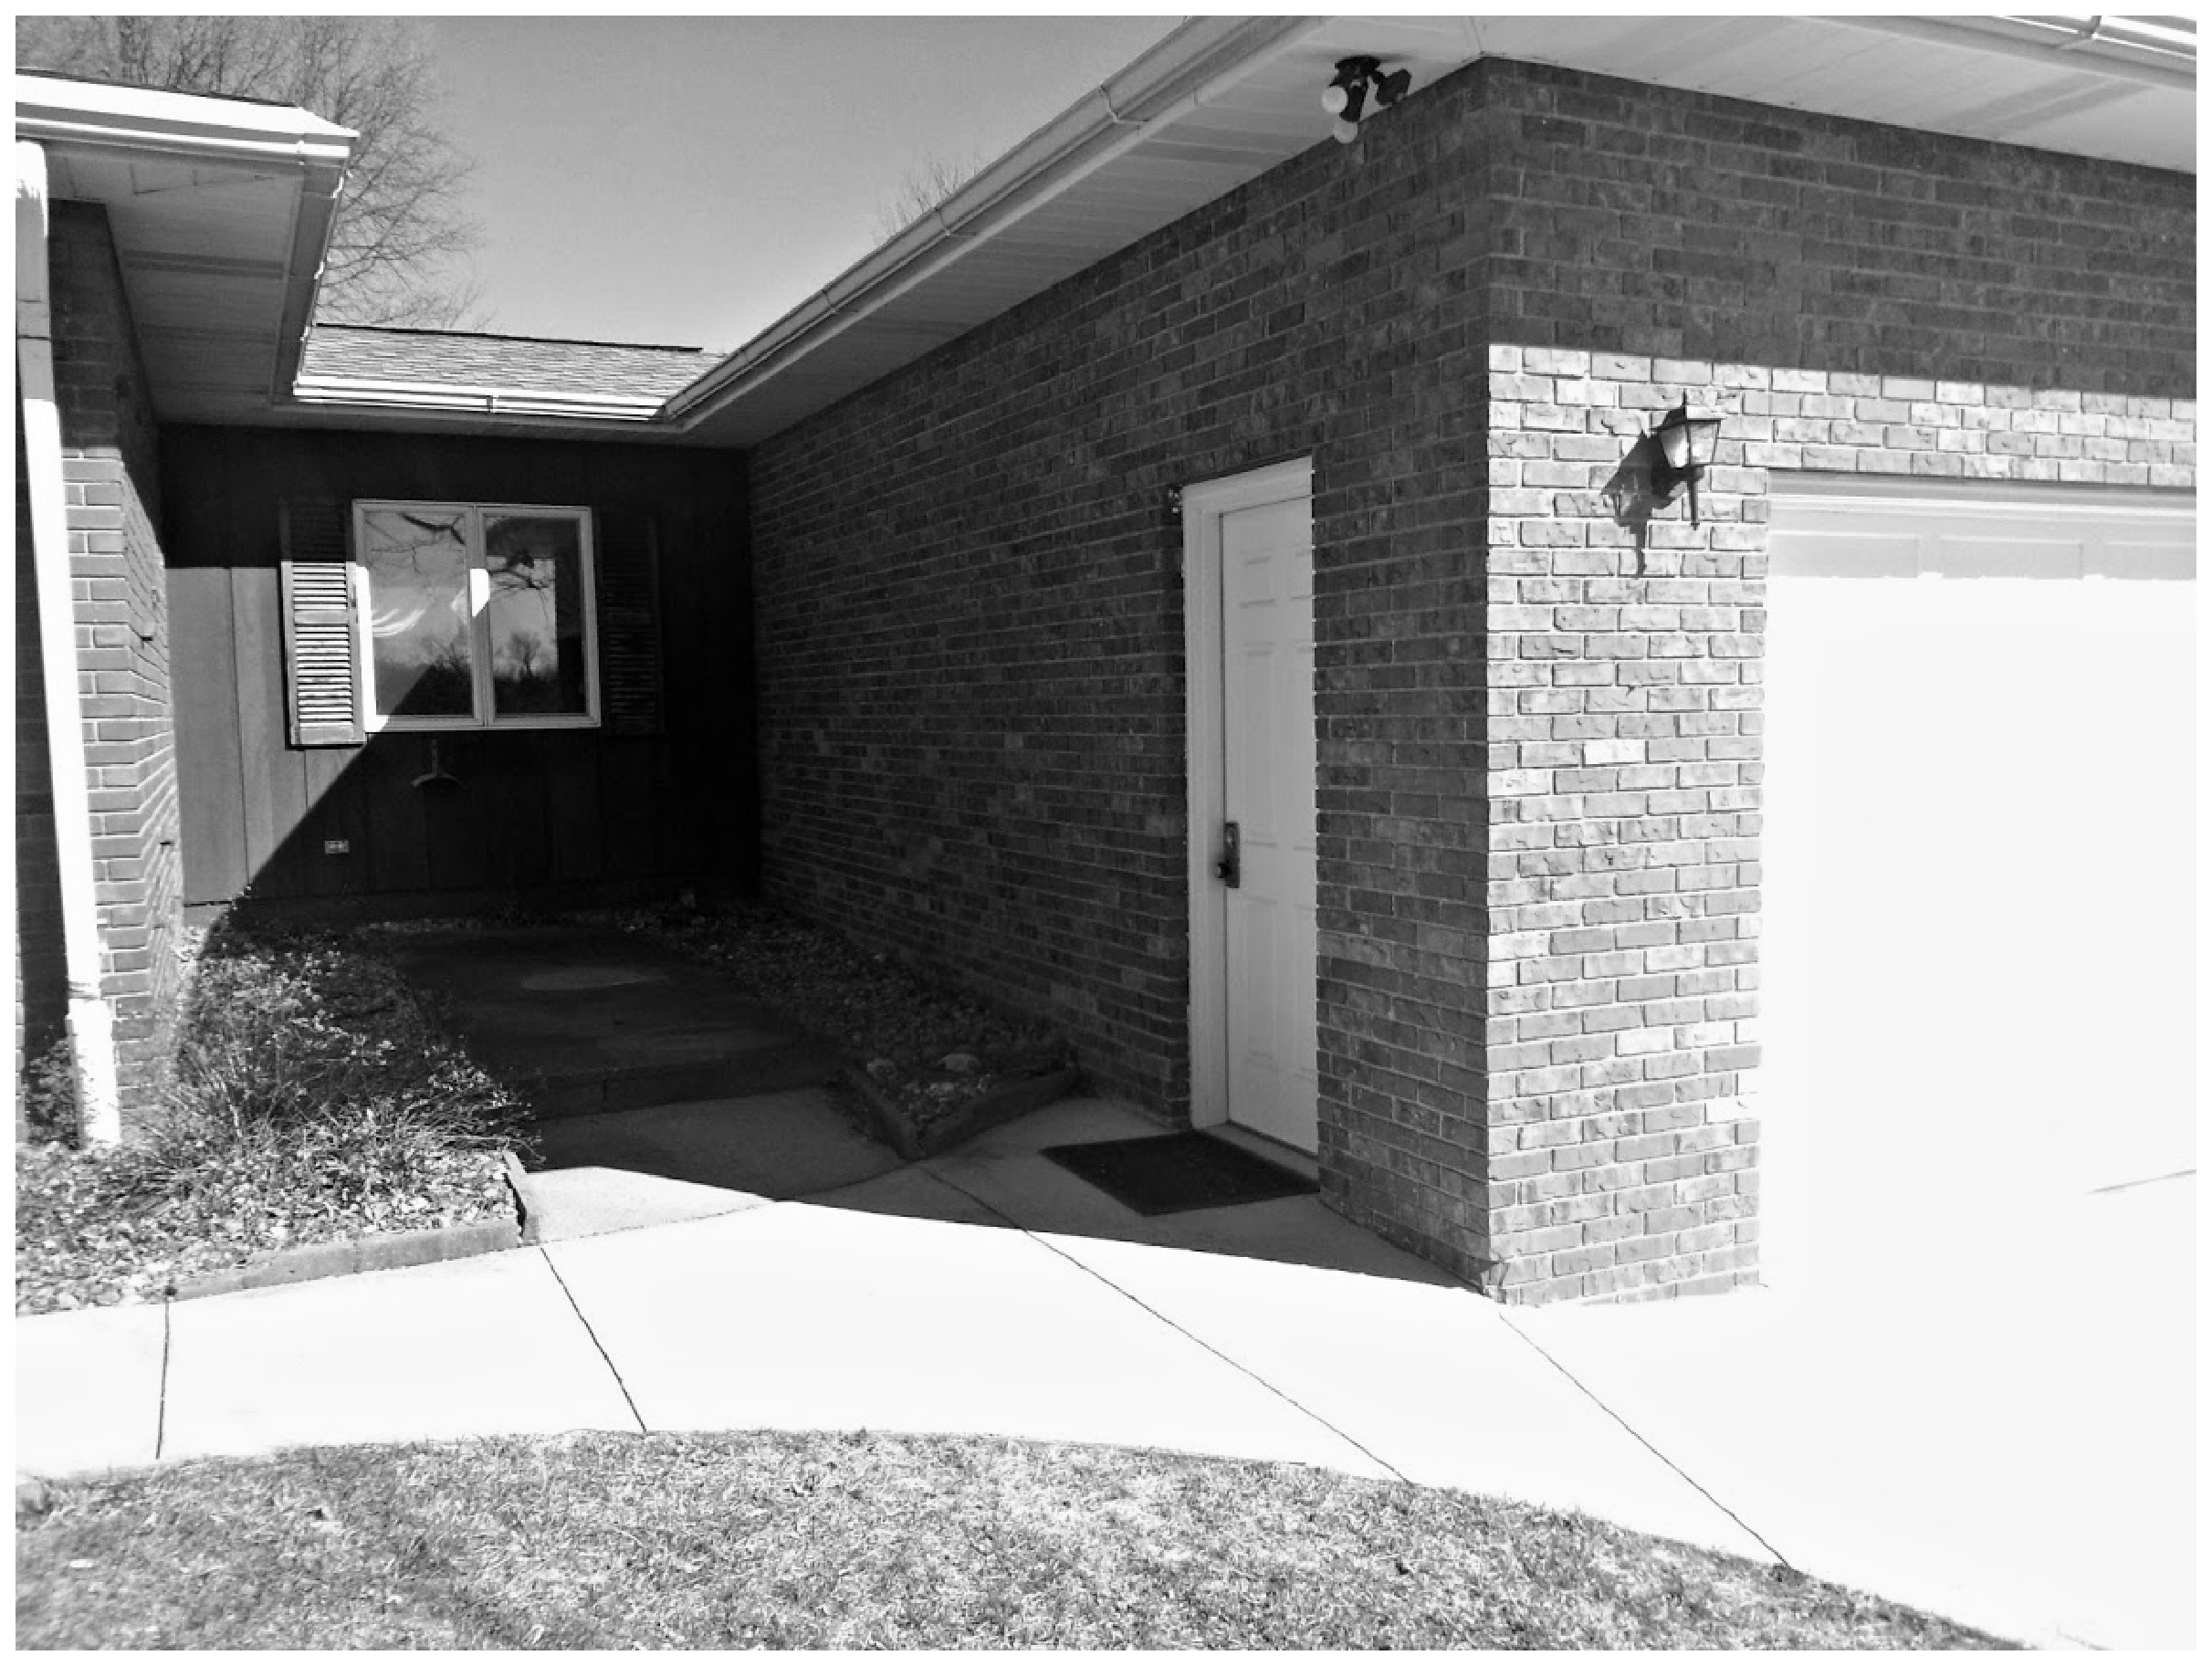
\includegraphics[width=.5\textwidth]{mullerlyerhouse}
\caption[Muller Lyer Real World Context]{The Muller-Lyer illusion in a non-ambiguous three-dimensional context.}\label{fig:mullerlyerhouse}
\end{figure}

Depth illusions in particular result from a conflict between our experience with the three-dimensional world and the appearance of two-dimensional ambiguous stimuli. The Necker cube ``flips" because there are two physical objects that could produce the same retinal image, the Muller-Lyer illusion exists because our experience with the three-dimensional world is harnessed inappropriately for a two-dimensional figure, and the color-constancy illusion exists because our brains automatically correct a pseudo three-dimensional image to represent the reality of that image in the real world. These conflicts occur in statistical graphics as well; Chapter \ref{sineillusion} explores statistical graphics that trigger a three-dimensional heuristic in the brain and lead to misleading conclusions.

There are other optical illusions that have the potential to appear in statistical graphics but are not easily classified (or necessarily easily explained). Two of these illusions are considered below.
\paragraph{Other Important Optical Illusions}
Certain illusions do not lend themselves to simple classification. While many illusions are the result of multiple concurrent processes in the brain, these illusions may not even be fully understood. The Poggendorff illusion, shown in figure \ref{fig:poggendorff}, is one such illusion. 

\begin{figure}[htbp]\centering
\includegraphics[width=.4\linewidth]{Poggendorff}
\caption[The Poggendorff Illusion]{The Poggendorff Illusion. The left figure shows a black line which is obscured by a grey rectangle; it appears that the blue line would intersect the black line if the rectangle were not present. In fact, the black line and the red line are co-linear, and the blue line is parallel to both other lines.}\label{fig:poggendorff}
\end{figure}

\citet{gregory1963distortion, gregory1997knowledge} suggests the Poggendorff illusion is similar to the Muller-Lyer illusion in that it results from misapplied depth cues, but \citet{green1963poggendorff, ward1977case} found no evidence that participants viewed this illusion in any three-dimensional context. Instead, \citet{green1963poggendorff} suggests that the illusion results from a tendency to perceive acute angles as less acute and obtuse angles as less obtuse than the image suggests. As the illusion disappears as the angle of the line segment approaches horizontal, this seems to be a reasonable explanation, but it is almost certainly not complete \citep{morgan1999poggendorff}, as the illusion survives in forms which do not preserve the acute angle intersections. Regardless, this illusion can make it difficult to read line graphs \citep{amer2005bias, poulton1985geometric} if proper precautions (use of reference lines and grid lines) are not taken.

The second of these illusions is the cafe wall illusion, shown in figure \ref{fig:cafewall}, named because this tile pattern is apparently common in cafes. 



\begin{figure}[htbp]\centering
\hfil
\begin{subfigure}[b]{.4\textwidth}\centering
  \includegraphics[width=\textwidth]{CafeWall}
  \caption{Original Cafe Wall Illusion}\label{fig:CafeWallOrig}
\end{subfigure}\hfil
\begin{subfigure}[b]{.4\textwidth}\centering
  \includegraphics[width=\textwidth]{fig-cafewall}
  \caption{Isoluminant Cafe Wall Illusion}\label{fig:CafeWallIso}
\end{subfigure}\hfil
\caption[Cafe Wall Illusion]{The Cafe Wall illusion. The lines between rows of black and white tiles are parallel but appear to be tilted. The second image shows the isoluminant version, which mitigates some of the illusion but does not entirely eliminate the effect.}\label{fig:cafewall}
\end{figure}

The cafe wall illusion is in part due to the contrast between light and dark zones (as in the mach bands and hermann grid illusion), and much of the illusion is resolved when the black and white tiles are replaced with isoluminant colors, but some of the illusion still remains. \citet{westheimer2007irradiation} suggests that this portion of the illusion is because the position of a black-white border will be biased to appear closer to the black side of its physical location, an effect which is compounded in the cafe wall illusion to produce the appearance of tilted lines. This illusion, while not explicitly found in most statistical graphics, shows that even simple (and pleasant) configurations of geometric objects can wreak havoc in the brain under the right circumstances. In fact, the illusion is so simple that it is also known as the ``Kindergarten illusion", but its cause is sufficiently complex that it has not been fully explained by psychologists or neuroscientists. 

\subsection{Cognitive Load}\label{cognitiveload}
It is fairly well established that statistical graphics are useful in part because they can replace long tables of data, summarizing information in a form that is much easier to understand and mentally maniuplate; as such, it would not be out of line to suggest that graphics require less cognitive load than tables of the same data. When we discuss cognitive load, we typically mean the limits in short-term memory, cognitive manipulation, attention, and mental bandwidth that bound our ability to take in new information and draw conclusions from that information. In this section, we will briefly discuss some of these considerations. 

\paragraph{Short Term Memory} A famous paper in memory and cognition \citep{miller1956magical} suggests that active memory can contain only 7 (plus or minus two) chunks of information. A chunk of information could be a single letter or number, a meaningful collection of several letters or numbers (e.g. a word or an area code), or an association. This limitation is important in designing information for graphical consumption. For instance,  the number of categories in legends should be limited to 7, to allow a viewer to store the associations within the legend and then use that information to understand the graph. Abuse of this limitation is referred to as a ``color mapping attack" in \citet{conti2005attacking}, a paper detailing the various ways to ``attack" a human visualization system. Similarly, viewers should not be expected to remember more than 7 ``chunks" of information from a single graph. Due to these limitations in memory, when a single color scale is used to represent more than one order of magnitude of variation, using a logarithmic scale provides more optimal information scaling than using a linear color scale \citep{sun2012framework, varshney2013we}. 

\paragraph{Information Integration}
Integrating multiple dimensions of information (or mentally combining multiple graphics) is another area which can strain the ability of the brain to utilize information effectively. Well-constructed graphs can help the brain to integrate information by connecting points across dimensions (through the use of regression lines, clustering, etc.), which creates ``chunks" of information that can then be stored in memory in a more compressed format. These chunks are useful because they allow people to draw conclusions from multiple sets of data across multiple dimensions \citep{gattis1996mapping}. Poorly created graphics may make this task harder or even promote the encoding of misleading chunks; for instance, data that is overplotted may obscure the important trend and may also produce chunks which lead to the wrong associations being stored in memory. This integration limitation is very much related to short-term memory, but is also constrained by mental effort limitations and processing capacity. As a result, it is important to reduce the effort required to integrate multiple graphics. 

\paragraph{Attention}
Human attention is limited; thus visualizations which do not focus attention on important aspects of the data are likely to confuse the reader. \citet{eda} said ``The greatest value of a picture is when it forces us to notice what we never expected to see". When there are too many salient features to notice anything in particular, attention is split too many ways to gain useful information from the picture. Graphics should present data in a controlled fashion, so that focused attention is rewarded with useful information taken from the graph. \citet{conti2005attacking} describes graphs that do not follow this principle as ``processing attacks", in that the overload the ``CPU" with needless calculations and mental manipulations that are ultimately futile to understanding the data. 

The consequence of the limits of human perception and processing capacity is that there is a limited amount of information one can expect to portray graphically; thus graphics should be designed to most efficiently communicate information so that this cognitive overload does not occur. The next section presents studies which examine the perception of graphs and charts directly across a wide range of perceptual levels and experimental conditions. 

\section{Statistical Graphics}
Psychologists who study graphical perception are generally concerned with the underlying mechanisms of effects within the brain, and thus study very simple graphics and lower-level perceptual effects. In statistics, the literature is somewhat more variable; \citet{cleveland:1985} produced the seminal paper on the subject, but outside of that work, there are relatively few papers that examine the accuracy of judgments made from graphs through user studies that mimic the way graphs are used in practice. There have been a few papers in other disciplines; business and communications researchers occasionally study graphs and charts as well. As a result, the literature in this area is scattered across many disciplines. In order to organize this section effectively, we will begin with the lower-level graphical perception literature and conclude with studies that have more external validity and are applicable to statistical practice. For the purposes of the following sections, lower-level perception research is research which involves either extremely simple graphical elements (or non-graphical research which applies directly to graph perception processes), or which does not require attention (pre-attentive features of graphics). These experiments provide some information, but are less informative than experiments which utilize more complex graphics in realistic scenarios. 

\subsection{Preattentive Perception of Statistical Graphics}\label{LowLevelGraphics}
Much of the lower-level research within the statistical graphics literature has been performed by those within the psychological community that study human information processing. In particular, \citet{healey1999large, healey2012attention} have produced several papers studying the accuracy of conclusions viewers can make after less than 1/2 of a second of viewing an image. As discussed in section \ref{AttentionPerception} and demonstrated in figure \ref{fig:preattentive}, certain features do not require individual focus to process; these features are called \emph{preattentive} and can be detected on the first glance (typically within 250ms). Healey's work focuses on determining which features can be detected in a pre-attentive fashion, and whether a hierarchy of features exists when these features are combined. Healey suggests that for three-dimensional displays, the 3d layout is determined first, surface structure and volume are determined next, followed by object movement (if present), luminance gradients, and color; he suggests that if there are conflicts between these 5 levels, priority is given to an earlier process \citep{healey2012attention}. \citet{healey1999large} showed that if visualizations are carefully constructed to conform to the architecture of the human visual system (isoluminant colors, removing certain background patterns from textural arrays), visual estimation tasks can be performed preattentively. The experiment also revealed an interference effect between texture and color that corresponds to previously documented interference between preattentive features \citep{treisman1985preattentive}. Figure \ref{fig:preattentiveinterference} demonstrates the interference effect; it is much easier to locate the target point in figure \ref{fig:preattentiveshape} or figure \ref{fig:preattentivecolor} than it is to locate the target in figure \ref{fig:preattentiveinterference}.






\begin{figure}[htbp]\centering
\begin{subfigure}[b]{.3\textwidth}\centering
  \includegraphics[width=\textwidth]{fig-preattentive11}
  \caption{Shape}\label{fig:preattentiveshape}
\end{subfigure}\hfill
\begin{subfigure}[b]{.3\textwidth}\centering
  \includegraphics[width=\textwidth]{fig-preattentive12}
  \caption{Color}\label{fig:preattentivecolor}
\end{subfigure}\hfill
\begin{subfigure}[b]{.3\textwidth}\centering
  \includegraphics[width=\textwidth]{fig-preattentive22}
  \caption{Interference}\label{fig:preattentiveinterference}
\end{subfigure}
\caption[Preattentive Features and Interference]{Shape and color are detected preattentively in figures (a) and (b), but interfere in figure (c) so that location of the target in (c) is no longer preattentive.}\label{fig:preattentive}
\end{figure}

Healey's work on preattentive perception is interesting, and provides a reasonable approach to creating graphics compatible with the human visual system, but his work is largely focused on multidimensional displays and his focus on preattentive processes limits the applicability of his work to statistical graphics. In particular, most graphics are created with the idea that a viewer will spend more than one second looking at the graph, so not all features need to be preattentive to be useful. In addition, many of the multidimensional displays he designs are very load-intensive to understand; with so many additional dimensions, the viewer must spend considerable time understanding the scales and legends which correspond to each variable. In the next section, we will examine the literature concerning higher-level graphical perception, including perception at the attentive level and which types of graphs are more accurately perceived by viewers. 

% \todo[inline]{Add section examining psychological literature (treisman) for lower-level measurement accuracy style studies?}

\subsection{Conscious Perception of Statistical Graphics}\label{HighLevelGraphics}
Graph perception from a statistician's point of view is more focused on the attentive stage of perception: When asked to answer a question using a graph, what parts of the graph are useful, and how is the information transferred from the image to working memory in the brain? Several models have been proposed to describe this process; of these, the set of ``task models" and ``integration models" seem to be most consistent with empirical evidence. 

\subsubsection{Models of Graph Perception}
These task-based models suggest that task-based graphical perception, e.g. using a graph to answer a specific question involves several stages of information processing \citep{ratwani2008thinking}. 
\begin{enumerate}
\item Parts of the question are read several times
\item The graph is searched for relevant information, with focus shifting from the graph axes to the main part of the graph and back again (pattern recognition)
\item Once information is found, the focus shifts between the important part of the graph and the legend several times in order to keep the relevant information in working memory (conceptual relations produce quantitative meaning from visual features)
\item The question is answered and the participant moves on to another task (the question is related to the encoded quantitative features)
\end{enumerate}

These steps are illustrated in figure \ref{fig:taskgraph}. 


\begin{figure}[htbp]
\textbf{Question:} What is the relationship between the length of the eruption and the time between eruptions for Old Faithful?
\begin{center}
\begin{minipage}[c]{.45\textwidth}
\includegraphics[width=\linewidth]{fig-steps}
\end{minipage}
\begin{minipage}[c]{.54\textwidth}
\textbf{Sample mental steps: }
{\small
\begin{enumerate}
\item Understand the question, identify ``length of eruption" and ``time between eruptions" as things to search for in the graph.
\item Look for ``length of eruption" on the axes, determine that the $y$ coordinate contains that information. Look for ``time between eruptions" on the axes and determine that the $x$ coordinate contains that information. Verify that these quantities are indeed what is being sought by re-reading the question. 
\item Establish that as the time between eruptions increases, the length of the eruption increases. Note that there seems to be a bimodal distribution of points. 
\item Answer the question: As the time between eruptions increases, the length of the eruption seems to increase.
\end{enumerate}
}
\end{minipage}
\end{center}
\caption[Task analysis of a simple graph]{Task analysis of a simple graph-based task. The graph shows the length of the eruption of Old Faithful as a function of the waiting time between eruptions, with a corresponding sample ``mental dialog" of the perceptual tasks involved in answering the question in response to the graph, according to \protect\citet{shah2005cambridge}. }\label{fig:taskgraph}
\end{figure}

Working within this task-oriented framework, researchers have explored the ``search" portion of the task-based model, the information integration portion of the model, and the types of graphs which facilitate both the ``search" and ``integration" portions of the task. Integration models modify the above sequence to allow for more complex graphical relationships to be assimilated, such that a viewer cycles between stages (2) and (3) several times in order to encode different portions of the graph. The time required for each of these steps may also change in accordance with the reader's familiarity with the task and graphic style; those who are more familiar with similar graphics may be able to encode information faster and in larger chunks and thus answer the question more quickly \citep{carpenter1998model}. 



\begin{figure}[htbp]\centering
\begin{subfigure}[b]{.45\textwidth}\centering
  \includegraphics[width=\textwidth]{fig-clustering1}
  \caption{Proximity-based grouping}
\end{subfigure}\hfill
\begin{subfigure}[b]{.45\textwidth}\centering
  \includegraphics[width=\textwidth]{fig-clustering2}
  \caption{Proximity and Similarity-based grouping}
\end{subfigure}\hfill
\caption[Chunking in Graphs]{The utility of chunking in graph perception. Graph (a) could potentially be described as three distinct clusters of points rather than 120 individual points, but it is much easier to draw conclusions from graph (b), which has colored points that clearly show the grouping structure in the data. The second figure would more probably be encoded and described as three groups of 40 points, which serves as a form of mental data compression.}\label{fig:clustering}
\end{figure}

Analyzing graphs using task-based models emphasizes the importance of spatial relationships between graphical elements. The gestalt laws of proximity and similarity dictate that items which are close together or physically similar (the same shape or color) are perceived as a group; this spatial perception creates ``chunks" of the graph which may be encoded as single objects and thus reduce the mental bandwidth necessary to process the image. Figure \ref{fig:clustering} shows the advantage of ``chunks" in graphs, as the second graph shown is much easier to describe and understand than the first graph, even without the contextual meanings of the variables. Of graphics that present information of similar complexity, graphics that require less effort to understand and search for relevant information are preferrable \citep{cleveland:1985}. More complex models of the graphical perception process suggest that data are integrated on a visual level and then further integrated on a cognitive level, to form successive clusters of information. Once these clusters are formed, further information can be integrated by comparing and contrasting different clusters to understand the higher-level meaning in the graph \citep{ratwani2008thinking}. Graph types which cater to this hierarchical clustering mechanism may be more easily understood by viewers than graphs that do not provide information in a manner easily assimilated by the human brain. Based on this information, facets of graphs may be particularly useful for mapping multidimensional data to provide ``chunks" of information in a relevant manner that can be integrated into the viewer's working conceptual understanding of the dataset. Additionally, color schemes and appropriate labeling of graph features which reduce the amount of work necessary to integrate numerical information from a legend into the visual representation of the graph facilitate graphical inference \citep{carpenter1998model}.

From a statistical perspective, much of the literature involved in understanding graph perception from a task-analysis point of view focuses on simple graphics, such as side-by-side bar graphs or line graphs, and straightforward tasks of reading information from the graph accurately, rather than examining model assumptions or making inference beyond the data. The psychologocial mechanisms involved in processing simple graphics are perceptual, and typically require direct comparisons rather than mental manipulation in order to satisfy the tasks posed by the researchers \citep{trickett2006toward}. More complicated graphics and more sophisticated tasks may require comparison of two or more distinct graphs and may utilize working memory and spatial reasoning; these situations are not as well studied \citep{shah2005cambridge}. We begin first with the simple tasks of graph comprehension, and will summarize work with more complicated graphics at the end of this section. 

\subsubsection{Perception of Simple Graphs}
A series of experiments by \citet{cleveland:1984, cleveland:1985} studied basic perceptual tasks in graphical perception to produce a relative ordering of graphical elements by the accuracy of participant conclusions. This ranking is shown in Table \ref{clevelandranking}. Other researchers \citep{kosslyn1994} have collapsed this ranking into position/length/angle and area/volume, as the difference in accuracy between categories 1, 2, and 3 is small compared to categories 4 and 5. 
\begin{table}[htbp]\centering
\begin{tabular}{ll}
\hline
Rank & Task\\\hline
1 & Position (common scale)\\
2 & Position (non-aligned scale)\\
3 & Length, Direction, Angle, Slope\\
4 & Area \\
5 & Volume, Density, Curvature\\
6 & Shading, Color Saturation, Color Hue\\\hline
\end{tabular}
\caption[Cleveland \& McGill's ordering of graphical tasks]{\protect\citet{cleveland:1984, cleveland:1985} ordering of graphical tasks by accuracy (adapted from both papers and \protect\citealt{shah2005cambridge}). Higher-ranking tasks are easier for viewers than low-ranking tasks and should be preferred in graphical design.}\label{clevelandranking}
\end{table}

The particular task required of participants in experiments also has an effect; \citet{simkin1987information} found that readers were more accurate in determining position when presented with a bar graph, but when readers were presented with a pie chart, they were more accurate at determining proportional judgments (using angles). This finding contradicts \citet{cleveland:1984} to some degree and suggests that the experimental design and specific task are important in evaluating these sorts of user studies; the contradictory results also suggest that graph type is an important influence in determining what information viewers encode from the graph. This conflict also illustrates that the user's attention and past experience influence the judgments they make from a given graph: when participants were asked to provide a summary of the graphic, their answers depended on the type of display: bar charts elicited a comparison judgment, pie charts elicited proportional judgments \citep{simkin1987information}. Similarly, when presented with a line graph, viewers are more likely to summarize the graph in terms of the slope of the trend line (even when the x-axis is discrete); when presented with a bar graph, viewers summarize the information using discrete comparisons \citep{carswell1987information, shah2005cambridge}. The task and the graph format interact to influence viewer perceptions, thus, when creating graphics, statisticians should match appropriate graphical formats to meaningful conclusions about the data. 

The task requirements are mediated by the limits of human processing ability. Chernoff faces, once proposed for visualizing multidimensional data, are difficult to read because viewers are unable to store the legend and the image in working memory; comparisons must be made serially and with conscious attention \citep{shah2005cambridge}. Similarly, while color does not generally correspond to precise quantitative information, certain color schemes utilizing hue, saturation, and brightness together can provide an implicit numerical ordering that does not place exceptional demands on working memory \citep{shah2005cambridge}. Color schemes which correspond to everyday situations (e.g. using a blue to red scale for low to high temperatures) may also reduce the demand on working memory. While specific numerical judgments would still require selective attention, the ``gist" of a graph using such schemes may be understood fairly quickly. 

Other graph features can also influence the inferences viewers make: multiple studies suggest that our mental schematic for a graph is most consistent with a $45^\circ$ trend line \citep{cleveland:88, tversky1989perceptual}. ``Banking to $45^\circ$" is a commonly-cited recommendation for optimal graphics, and does have some limited utility in reducing the strength of the line-width illusion (a more thorough discussion of this heuristic is provided in Chapter \ref{sineillusion}). Axis scale transformations can make it easier for viewers to spot outliers of data conforming to skewed distributions (though this does require some domain-specific knowledge of statistical distributions), and appropriately labeled graphs can reduce the working memory requirements by reducing the number of ``back-and-forth" comparisons required to pass information into working memory \citep{shah2005cambridge}. 

These studies indicate that it is important to consider the cognitive processing of statistical graphics as well as the data used to generate these graphics: the type of graph, color scheme, annotations, aspect ratio, legends, and axis transformations can all influence the amount of mental processing required to draw conclusions from a graph, as well as the types of conclusions that graph viewers are likely to draw. Many of these features were studied in relative isolation, using simple graphs that may lack real-world context. More complex, domain specific graphs may require higher cognitive load and may promote recruitment of previously acquired knowledge; experiments using simple, bland graphics may not be applicable to more complex graphics meant for experts. What follows is a summary of the relatively sparse literature on these sorts of real-world graphics. 

\subsubsection{Perception of Complex, Domain-Specific Graphs}
\citet{carpenter1998model} showed that graph comprehension time increased when the number of distinct x-y  functions (i.e.  nonparallel sloped lines) increased, even if the same data was represented. The density of these functions also had an impact: dense graphs with multiple intersecting trend lines took more time to interpret than dense graphs with parallel trends or sparse graphs with intersecting trend lines. This supports the idea that the information conveyed in the graph must be read into working memory before the graph can be described or used for inference; more complex graphs would take more time to understand and internalize. Additional factors can also influence the ease with which graphs are perceived and understood in real-world scenarios. \citet{gattis1996mapping} found that graphs were more accurately perceived when the dependent variable was on the y axis and the independent variable was on the x axis, even when the perceived IV and DV were manipulated using a cover story. In even more complex visualizations, \citet{trickett2006toward} found that meterologists and other domain experts would mentally superimpose graphs from memory on visible graphs, utilizing spatial processing rather than manipulating a physical interface. These interactions demonstrated complex spatial manipulation to assimilate information from multiple graphs, particularly when the information provided in the graphs conflicted with prior information, either from the meterologist's own domain knowledge or verbal information provided during the course of the study. While the procedures used in this study rely on verbal descriptions of mental processes (i.e. the meterologist speaking aloud as they process each graph and map to assimilate information), the evidence is sufficient to suggest that in addition to working memory and the visual processing performed by the brain, some complex graphs also utilize spatial processes (and the corresponding brain regions) to perform complicated overlays and mental transformations. By designing such complicated graphs to more easily facilitate such mental operations, it is possible that more effective spatial visualizations could make these graphs more accessible. 

Complicating the research into more complex graphs, there are many different types of complexity that can affect graphics. There may be differences in how processing occurs for large amounts of data, but it could also be that more complex x-y relationships could also require more mental effort. In addition, multiple relationships can be depicted simultaneously, either because of underlying groups in the data or because multiple related trends are depicted on the same graph (though this is widely acknowledged as bad practice in statistical graphics). Finally, the mental complexity of the task required of the graph viewer can also factor into the amount of time and effort required to complete a task using a graph. These different types of complexity interact with the graph format; for instance, line graphs are less effected by increasing complexity than bar graphs \citep{tan1994human}, and bar graphs are more affected by increasing complexity than pie charts for ratio judgments \citep{hollands1998judging}. 

Finally, complex graphs often facilitate different types of participant tasks; rather than simple numerical judgments or information lookup, complex graphs may encourage (or require) viewers to use prior knowledge and interpretation skills. These additional complications make experimental study of complex or domain-specific graphs more difficult. Many of these problems (types of complexity, expanded tasks, prior knowledge) make further work in this area somewhat difficult. One concept that facilitates studies examining the relationship between complex data and graph format in statistical graphics is the \emph{grammar of graphics}, which we discuss in the next section, along with other experimental methodology useful for understanding how people perceive statistical graphics. 

% \subsection{Interactive graphics?} 
% Not sure if this should be a subsection, but graphics that respond to human interaction violate the two-dimensional graphic paradigm somewhat, which means there are a whole 'nother set of issues to consider... motion illusions, grouping, etc.

\section{Testing Statistical Graphics}
\subsection{Basic Psychophysics Methodology}
Psychophysics studies are generally concerned with the ability to detect a stimulus (or a difference between two stimuli). Many classic psychophysical methods are still used in studies today (for an example, see Chapter \ref{sineillusion}). Several of these methods are mentioned here; for a more thorough review, see \citet{goldstein}. 
\paragraph{Method of Limits} The method of limits seeks to determine the level of intensity at which a stimulus is just barely detectable. A series of trials is used, with each trial starting at either the lower or upper range of intensity and incrementally moving towards the opposite end of the range; for each point, the observer indicates whether they can detect the stimulus. At the end of several trials, the detection limits are averaged to produce a measured \emph{absolute threshold}. Figure \ref{fig:methodoflimits} demonstrates this process. 



\begin{figure}[htbp]\centering
\includegraphics[width=.5\textwidth]{fig-methodoflimits}
\caption[The Method of Limits]{Demonstration of the method of limits. In this experiment, three trials were performed, two trials starting from 0 and increasing, and one trial starting at 9.5 and decreasing. The empirical detection threshold is the threshold at which detection occurs 50\% of the time, and is shown in red. }\label{fig:methodoflimits}
\end{figure}

\paragraph{Method of Adjustment} This method is similar to the method of limits, except that the stimulus intensity is adjusted by the observer (not the experimenter) in a continuous manner until the observer can just barely detect the stimulus. This procedure may be repeated several times, with trials averaged to produce a mean value for the absolute threshold. Figure \ref{fig:methodofadjustment} demonstrates this procedure. 


\begin{figure}[htbp]\centering
\includegraphics[width=.5\textwidth]{fig-methodofadjustment.pdf}
\caption[The Method of Adjustment]{Demonstration of the method of adjustment. In this experiment, four trials were performed, two trials starting from 0 and increasing, and two trials starting at 10 and decreasing. The empirical detection threshold is the threshold at which detection occurs 50\% of the time, and is shown in red. \label{fig:methodofadjustment}}
\end{figure}

\paragraph{Measuring the Difference Threshold} The difference threshold, discussed in section \ref{logarithmicperception}, is the smallest detectable difference between two stimuli. This threshold can be measured using either the method of limits or the method of adjustment. Rather than increasing the absolute intensity of the stimulus as discussed above, two stimuli are given: one with constant intensity and one whose intensity may vary either continuously or incrementally (depending on the method utilized). The participant is instructed to identify the point at which the two stimuli are indistinguishable (if the varied stimulus is approaching the constant stimulus) or the point at which the two stimuli are distinguishable (if the varied stimulus is diverging from the constant stimulus). 

\paragraph{Magnitude Estimation} Magnitude estimation studies are used to measure the perceptual intensity of two different stimuli. For example, a participant might be shown a series of two lights, and asked to assign a number to describe how bright each light is. These numerical values would then be compared to the actual light intensity (as measured by a digital sensor or by the input voltage) to determine how perceived brightness corresponds to actual intensity. Many stimuli measured this way produce power-law functions that exhibit response compression (doubling the actual intensity corresponds to a much smaller change in perceived brightness) or response expansion (doubling the actual intensity corresponds to a change in perceived intensity that is more than double the original intensity). 

\subsection{Testing Images using Psychological Paradigms}
In addition to the psychophysics methods outlined above, there are testing paradigms within psychology that are applicable to the study of statistical graphics. These include experimental methods such as visual search and eye tracking, as well as experimental control procedures that may be important in graphics studies that are similar to cognitive psychology studies. We will first discuss the experimental methods, and then briefly discuss some common control procedures that may be applicable to the study of statistical graphics. 

\subsubsection{Experimental Methods}\label{experimentalmethods}
Many psychological experiments utilize straightforward methods to address hypotheses in perception, such as asking participants to make numerical judgments based on presented stimuli. These methods are quite useful, but not particularly difficult or domain-specific. In this section, we discuss two domain-specific methods for understanding perception of visual stimuli: visual search and eye tracking. 

\paragraph{Visual Search} Simply put, visual search methods involve presenting a participant with many distractor stimuli and one or more target stimuli, and asking the participant to locate the target stimuli. Time is measured between the initial stimulus presentation and the participant's answer; participant accuracy is also considered in more complicated visual search settings. This procedure allows researchers to measure simple preattentive stimuli and can also be utilized for more complicated tasks that require attention \citep{anderson1983interactive}. One example of a visual search task is shown in figure \ref{fig:visualsearch}; a common preattentive search task is shown in figure \ref{fig:preattentiveinterference}. 

\begin{figure}[htbp]\centering
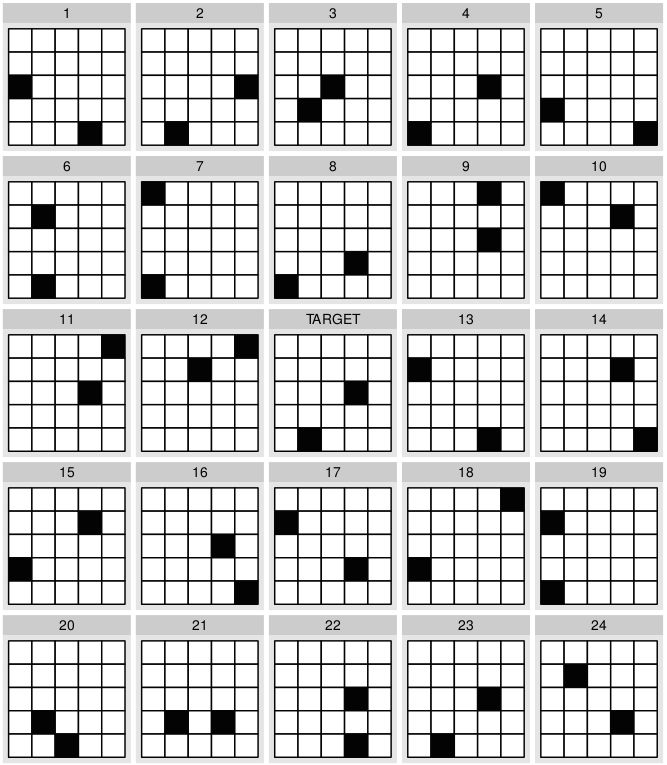
\includegraphics[width=.7\textwidth]{VisualSearch}
\caption[Visual Search Task]{Visual Search Task. Participants were asked to locate the figure (1-24) most similar to the central ``target" figure.}\label{fig:visualsearch}
\end{figure}

Visual search tasks can be used to measure the efficiency of a participant's visual search abilities (and focus on a task) to serve as a baseline for more complicated visual tasks. They can also be used to examine feature binding and common mistakes that may indicate relevant distractor stimuli. Even when reaction time is not directly measured, these tasks are typically given under time pressure, to establish a baseline performance that is below 100\% performance on the task. This time pressure allows experimenters to avoid response compression, so that the number of questions completed within the time limit provides an approximate measure of response time.

\paragraph{Eye Tracking} \label{eyetracking}
Eye tracking studies are often utilized in order to understand which parts or features of an image participants focus on, and in what order they examine the image components. Eye tracking studies were heavily used in order to refine the task-based models of graphical perception; they allowed researchers to understand that participants had to iterate between the question and different parts of the graph in order to assimilate all of the represented information into working memory. Figure \ref{fig:eyetracking} shows one lightweight eye-tracking assembly. The camera allows researchers to track the direction of the pupil and thus infer gaze direction. 

\begin{figure}[htbp]\centering
\includegraphics[width=.4\textwidth]{EyeTrackingGear}
\caption[Eye Tracking Equipment]{Eye tracking equipment \protect\citep{babcock2004building}. The cameras allow researchers to determine what part of a scene the wearer is viewing.}\label{fig:eyetracking}
\end{figure}

Eye tracking studies have been performed on statistical graphics as well \citep{zhao2013mind}, utilizing a visual search task and examining which graphics participants compared to determine the target plot.

In some psychological experiments, the straightforward approach to a task can produce biased responses from participants. Human perception is highly reliant on expectations and past experience, and as a result, experimenters must take care to reduce undesired biasing effects in order to appropriately control experiments. Some of these considerations are discussed in the next section. 
\subsubsection{Experimental Control Procedures}
While not all of the experimental control procedures discussed here are appropriate for every experiment, they do demonstrate the degree of control many experiments require to measure small psychological effects. The variation in the human brain and in cognitive strategies (and the sample size constraints of testing in humans) requires a large degree of experimental control in order to minimize the effects of population variance. Some of the biases of the human brain as well as strategies to address these biases are described below.

\paragraph{Habituation} The human visual system is attracted to novelty; odd, bizarre, or new sights attract more attention than ordinary, run of the mill scenes. Habituation describes the process of becoming less interested in a stimuli; as this occurs, the mind begins to enter ``auto-pilot" and attention to the task at hand becomes less focused. In infants, this habituation process is used to determine whether there is a perceived difference between two stimuli; in adults, this process is not typically as useful to the experimenter. To avoid habituation, experiments should generally consist of somewhat varied tasks in order to maintain participant attention. The psychophysics experiments described in figures \ref{fig:methodoflimits} and \ref{fig:methodofadjustment} can be vulnerable to this problem; to overcome habituation, trials often alternate in direction or start at random points along the intensity spectrum. 

\paragraph{Masking} Images can persist on the retina for a period after the image is no longer available; this phenomenon is called \emph{persistence of vision}. In order to control the time in which the stimulus is visible, psychological experiments often will show a mask immediately after an image in order to ``erase" the retina. This degree of control is often useful in experiments which focus on the preattentive stage of perception, but persistence of vision is not likely to affect experiments which take place in the attentive stage of perception (i.e. images shown for more than .5 seconds). A sample mask is shown in figure \ref{fig:mask}. 


\begin{figure}[htbp]\centering
\includegraphics[width=.3\textwidth]{fig-mask}
\caption[Sample Image Mask]{Sample mask used to ``erase'' the retina in some psychological experiments which test stimuli for short time periods ($<$1 s). The mask removes any afterimage the participant might have, ensuring that the stimuli is only available for the specified period. }\label{fig:mask}
\end{figure}

\paragraph{Priming} Broadly, priming is a technique that can be used to subconsciously bias a participant towards a certain conclusion. In cognitive psychology research, priming can be used to test word association (i.e. participants are quicker to identify an apple if they have just heard the word ``fruit" than if they heard the unrelated word ``pen"); in statistical graphics, priming effects are more likely to occur due to instructions or examples provided to participants at the start of a testing session. If an initial example contains notable outliers, participants are more likely to look for and recognize graphs with outliers than graphs with other notable features. Examples must be designed in such a way to avoid activating these priming affects as much as possible. 

There are many other psychological mechanisms that may impact participant performance; the mechanisms presented here are simply some of the more salient considerations in experimental design for statistical graphics. 

\subsection{Testing Statistical Graphics}
This section details the tools specific to the testing of graph perception within the field of statistics. \citet{cleveland:1985} studied statistical graphics from a largely psychological perspective, but their findings have been widely utilized in the field of statistics; however, it has been 20 years since that paper, and the field has developed within statistics since that time. Two major developments, the grammar of graphics and the lineup protocol, are particularly important for future research into the perception of statistical graphics. 

\subsubsection{The Grammar of Graphics}
The grammar of graphics, detailed in \citet{wilkinson2006grammar}, is a framework for describing a graphic in terms of its basic component pieces. An implementation of the grammar of graphics for R, \texttt{ggplot2}\citep{ggplot2, wickham2010layered}, provides a useful tool for manipulating graphics to test in an experimental setting. Using the grammar of graphics, it is easy for experimenters to compare different types of charts using the same data, as the underlying structure of the graph remains the same. Figure \ref{fig:grammarplots} shows three plots created using the same data and different geometric objects, and figure \ref{fig:grammarcode} provides the ggplot2 code to create the plots \footnote{These plots are terrible from a psychological perspective, but serve to illustrate the versatility of the grammar of graphics. In general, stacked density plots, histograms, and dot plots are bad for making numerical comparisons \citep{cleveland:1985}.}. Comparing these graphics experimentally would be reasonably simple, and the grammar of graphics helps to control the extraneous variables introduced by utilizing different plot types. In addition, the grammar of graphics approach to transformations and scales allows us to easily test judgments made utilizing different axis transformations and color scales to compare perceptual accuracy \citep{hofmann2012graphical}. 



\begin{figure}[htbp]\centering
\begin{subfigure}[b]{.33\textwidth}\centering
  \includegraphics[width=\textwidth]{fig-irisdatagrammar1}
  \caption{Stacked Density Plot}
\end{subfigure}\hfill
\begin{subfigure}[b]{.33\textwidth}\centering
  \includegraphics[width=\textwidth]{fig-irisdatagrammar2}
  \caption{Dotplot}
\end{subfigure}\hfill
\begin{subfigure}[b]{.33\textwidth}\centering
  \includegraphics[width=\textwidth]{fig-irisdatagrammar3}
  \caption{Histogram}
\end{subfigure}\hfill
\caption{Three different plots of iris data, created using the grammar of graphics}\label{fig:grammarplots}
\end{figure}

\begin{figure}[htbp]\centering
\begin{knitrout}
\definecolor{shadecolor}{rgb}{0.969, 0.969, 0.969}\color{fgcolor}\begin{kframe}
\begin{alltt}
\hlcom{# Stacked Density plot}
\hlkwd{ggplot}\hlstd{(}\hlkwc{data}\hlstd{=iris,} \hlkwd{aes}\hlstd{(}\hlkwc{x}\hlstd{=Sepal.Width,} \hlkwc{fill}\hlstd{=Species))} \hlopt{+}
  \hlkwd{geom_density}\hlstd{(}\hlkwc{position}\hlstd{=}\hlstr{"stack"}\hlstd{)}

\hlcom{# Dotplot }
\hlkwd{ggplot}\hlstd{(}\hlkwc{data}\hlstd{=iris,} \hlkwd{aes}\hlstd{(}\hlkwc{x}\hlstd{=Sepal.Width,} \hlkwc{fill}\hlstd{=Species))} \hlopt{+}
  \hlkwd{geom_dotplot}\hlstd{(}\hlkwc{method}\hlstd{=}\hlstr{'histodot'}\hlstd{,} \hlkwc{stackgroups}\hlstd{=}\hlnum{TRUE}\hlstd{)}

\hlcom{# Histogram}
\hlkwd{ggplot}\hlstd{(}\hlkwc{data}\hlstd{=iris,} \hlkwd{aes}\hlstd{(}\hlkwc{x}\hlstd{=Sepal.Width,} \hlkwc{fill}\hlstd{=Species))} \hlopt{+}
  \hlkwd{geom_histogram}\hlstd{(}\hlkwc{position}\hlstd{=}\hlstr{"stack"}\hlstd{)}
\end{alltt}
\end{kframe}
\end{knitrout}
\caption{ggplot2 code to produce figure \protect\ref{fig:grammarplots}}\label{fig:grammarcode}
\end{figure}

\subsubsection{Testing Statistical Graphics using Lineups}
One useful tool for testing statistical graphics is the concept of a lineup. Lineups combine the psychological notion of visual search tasks with the statistical concept of hypothesis testing: Participants are provided with a number of plots of the same form, one using real data and the rest generated using resampling methods. If participants identify the target plot (the plot with real data), this is considered similar in nature to a significant hypothesis test at a given $\alpha$ level (generally, there are 20 plots, so $\alpha=0.05 = 1/20$). Figure \ref{fig:lineupexample} shows a sample lineup. 



\begin{figure}[htbp]\centering
\includegraphics[width=.75\textwidth]{fig-irislineup}
\caption[Lineup for testing statistical graphics]{Lineup of the iris data, comparing sepal width to petal width. The target data is in plot 5, other plots generated by permuting petal width.}\label{fig:lineupexample}
\end{figure}
In addition to the visual inference protocols lineups were designed to fulfill \citep{buja2009statistical}, they also provide a method to easily quantify (on a statistical level) the ``power" of a plot; if two lineups are generated from the same data, but one allows participants to more frequently detect the target plot, then that lineup provides more perceptual power. The lineup protocol provides a useful tool for examining some of the issues discussed for complex, domain specific graphs. When combined with the grammar of graphics approach \citep{wickham2010graphical}, lineups have the potential to be extremely useful for studying the perception of graphs which present the same data in different forms.


\graphicspath{{Figure/sineIllusion/}{Images/sineIllusion/}}
\renewcommand{\floatpagefraction}{.99}

\newcommand{\range}[1]{{\text{range}\left(#1\right)}}
\newcommand{\s}[2]{{_{#1}s^{ #2}}}
\newcommand{\atan}[1]{\text{atan}\left({#1}\right)}
\newcommand{\xR}{\mathbb{R}}








\chapter{SIGNS OF THE SINE ILLUSION -- WHY WE NEED TO CARE}\label{SineIllusionChapter}\label{sineillusion}
%% Abstract
% Graphical representations have to be true to the data they display. Computational tools ensure this on a technical level. But we also need to take `flaws' of the human perceptual system into account. The sine illusion provides an example where human perception leads to systematic bias in the assessment of the optical stimulus, with a particularly notable impact on perception of time-series data with a seasonal component. In this paper, we discuss the reasons for the illusion and various strategies  useful to break the illusion or reduce its strength. We demonstrate the presence of the illusion in real-world and theoretical situations. We also present data from a user study which demonstrate the dramatic effect the sine illusion can have on conclusions drawn from displayed data.


\section{Introduction}
Graphics are powerful tools for summarizing large or complex data, but they rely on the main premise that any graphical representation of the data has to be ``true'' to the data (see e.g. \citet{tufte, wainer:2000, robbins:2005}). That is, a measurable quantity of a graphical element in the representation has to  directly reflect some aspect of the underlying data. Generally, we see a lot of discussion on keeping true to the data in the framework of (ab)using three dimensional effects in graphics. \cite{tufte} goes as far as defining a {\it lie-factor} of a chart as the ratio of the size of an effect in the data compared to the size of an effect shown, with the premise that any large deviations from one indicate a misuse of graphical techniques. Computational tools help us ensure technical trueness -- but this brings up the additional question of how we deal with situations that involve innate inability or trigger learned misperceptions in the audience. In this paper we want to raise awareness for one of these situations, show that it occurs frequently in our dealings with graphics and provide a set of strategies for solving or avoiding it.



\begin{figure}[h!tbp]\centering
\begin{subfigure}[b]{.45\textwidth}
  \centering
  \includegraphics[width=\textwidth]{fig-example1}
  \caption[Scatterplot of Ozone and Temperature in Houston, 2011.]{\small Scatterplot of Ozone and Temperature in Houston, 2011. A loess fit is overlaid to show the overall trend.  \label{fig:example1}}
\end{subfigure}\hfill
\begin{subfigure}[b]{.45\textwidth}
  \centering
  \includegraphics[width=\textwidth]{fig-example2}
  \caption[Residual Ozone]{\small Scatterplots of Ozone and Temperature de-trended according to the loess fit in (a). \\ \phantom{text to get to the next line}
  \label{fig:example2}}
\end{subfigure}
\caption[Scatterplots of Ozone and Temperature in Houston, 2011]{\label{fig:exampleFull1} Scatterplots of Ozone and Temperature in Houston, 2011. The increase in variability over the temperature range is more pronounced in the de-trended plot on the right.}
\end{figure}

As a first example let us consider the relationship between ozone concentration and temperature. Ozone concentrations were measured from 21 locations in the Houston area \citep{epa}, and temperature data is provided by the NCDC \citep{noaa} site at Hobby International Airport, located near the center of Houston. 

Figure~\ref{fig:example1} shows daily measurements of 8-hour average ozone concentration and temperature at several sites in Houston, for days in 2011 with temperatures above $45^\circ$F  and dew points of less than $60^\circ$F. 
A loess smooth line is added for reference. 
These types of plots are often used to give an overview of the relationship between two variables. The trendline summarizes this relationship, while the points show raw measurement to allow an assessment of the overall size of the data, the amount of (marginal) variability presented, as well as the (conditional) variability along the trendline. It is the latter task that we cannot satisfactorily complete. While we might agree that there is an increase in variability of ozone concentrations for temperatures above $80^\circ$F, we will not doubt homogeneity  elsewhere based on figure~\ref{fig:example1}. 


This evaluation changes when considering figure~\ref{fig:example2}: the scatterplot shows a loess based de-trended residual of temperature. A previously almost invisible increase in variability of ozone measurements with increasing temperatures now becomes apparent.

This phenomenon, caused by the change in the slope of the trend line,  is  known as the  {\it sine illusion} in the literature on cognition and human perception  or {\it line width illusion} in the statistical graphics literature. 

The illusion is a frequent occurrence in statistical graphics, and  displays should therefore be thoughtfully considered to minimize its effect visually and acknowledge its influence. 
In the cognitive literature, \citet{day:1991} first documented the illusion in the context of vertical lines along a sinusoidal curve. Figure~\ref{fig:original} shows a sketch of this: line segments are centered evenly spaced along the curve. Line segments are of equal length but appear longer in the peaks and troughs due to the illusion. The parameters that influence the strength of the illusion are the amplitude of the curve and the length of the line segments. As the length of the line segments increases,  the apparent difference in the length of the line segments decreases. Any modification that increases the change in slope under which the curve appears, such as an increase in the amplitude of the curve or a more extreme aspect ratio, reinforces the apparent difference in line lengths. 





\begin{figure}[hbtp]
\centering
\begin{knitrout}
\definecolor{shadecolor}{rgb}{0.969, 0.969, 0.969}\color{fgcolor}

{\centering 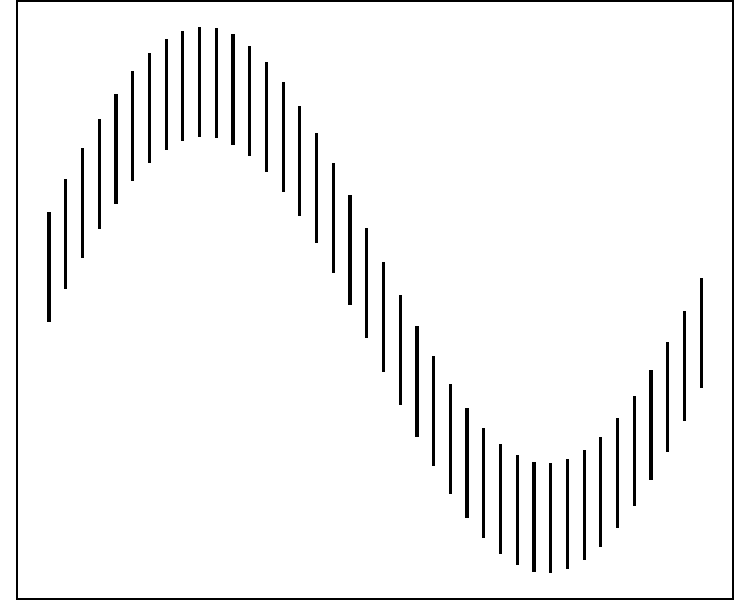
\includegraphics[width=.4\textwidth]{../Figure/sineIllusion/fig-original-1} 

}



\end{knitrout}
\caption[The original sine illusion]{The original sine illusion, demonstrated on evenly spaced vertical lines centered around a sinusoidal curve of $f(x) = \sin(x)$. The lines in the peak and trough of the curve appear to be longer than in the other regions.\label{fig:original}}
\end{figure}

More recently the illusion has been shown in non-sinusoidal curves \citep{cleveland:1984, schonlau:2003, robbins:2005, parallelsets}, but the underlying effect seems to be the same, in the sense that the illusion is not triggered by the periodic nature of the underlying trendline but only by  changes to its slope. Figure \ref{fig:twoillusions-simulation} shows three panels, which all exhibit the illusion. From left to right, the trend stems from (a) a periodic function, (b) a periodic component added to an exponential function, and (c) an exponential function on its own.
While all three graphs seem to show nonconstant variance along the main trend; in reality, it is constant. Clearly, the illusion does not rely on the periodicity of the function for which it was named, but is a symptom of the change in curvature that comes with the periodicity.

\begin{figure}[h!tbp]\centering
\begin{subfigure}[b]{.31\textwidth}
  \centering
\begin{knitrout}
\definecolor{shadecolor}{rgb}{0.969, 0.969, 0.969}\color{fgcolor}

{\centering 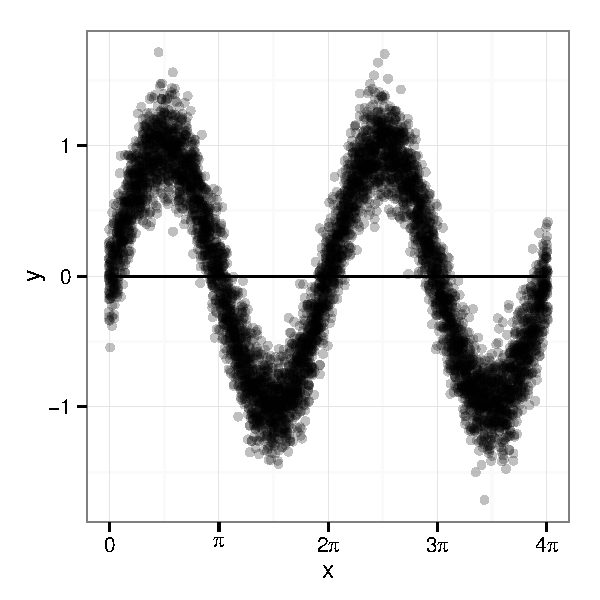
\includegraphics[width=\textwidth]{../Figure/sineIllusion/fig-simulation1Sine-1} 

}



\end{knitrout}
  \caption{\small Seasonality, No Trend}
  \label{simulation1}
\end{subfigure}
\begin{subfigure}[b]{.31\textwidth}\centering
\begin{knitrout}
\definecolor{shadecolor}{rgb}{0.969, 0.969, 0.969}\color{fgcolor}

{\centering 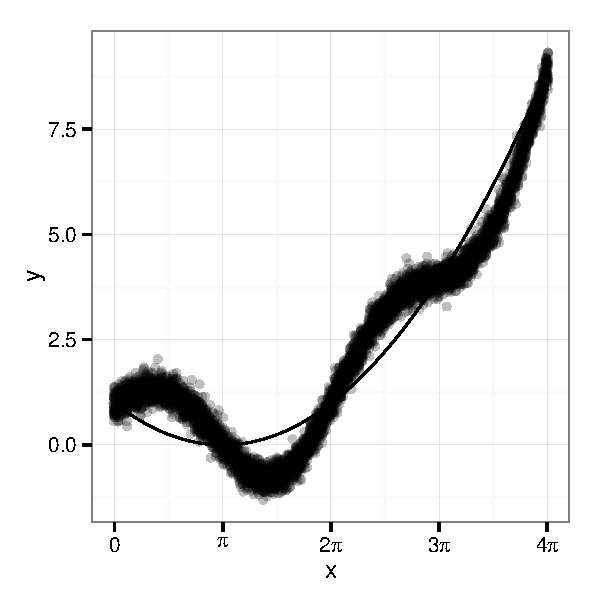
\includegraphics[width=\textwidth]{../Figure/sineIllusion/fig-simulation1Sine2-1} 

}



\end{knitrout}
  \caption{\small Seasonality and Trend}
  \label{simulation2}
\end{subfigure}
\begin{subfigure}[b]{.31\textwidth}\centering
\begin{knitrout}
\definecolor{shadecolor}{rgb}{0.969, 0.969, 0.969}\color{fgcolor}

{\centering 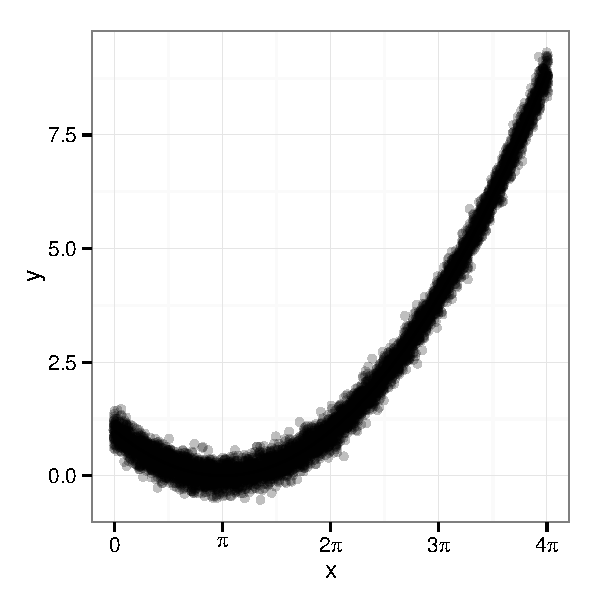
\includegraphics[width=\textwidth]{../Figure/sineIllusion/fig-simulation1Sine3-1} 

}



\end{knitrout}
  \caption{\small Trend, No Seasonality}
  \label{simulation3}
\end{subfigure}
\caption[Trend, seasonality, and the sine illusion]{Set of three scatterplots of simulated data with constant variance. Plot (a) shows seasonality without any underlying trend, (b) shows seasonality superimposed on a quadratic trend, and (c) shows a quadratic trend without seasonality. Though all three sets of simulated data have constant variance, none of the variances appear constant due to the sine illusion.}\label{fig:twoillusions-simulation}
\end{figure}

Next, we give an overview of the perceptual and statistical literature regarding this illusion.
\subsection{The Sine Illusion in Statistical Graphics}\label{statisticalgraphics}\hfill\newline
The sine illusion demonstrated in figures \ref{fig:exampleFull1} and \ref{fig:original} has been frequently noted in statistical graphics, though usually not as an optical illusion. Rather, the problem is typically identified as the difficulty of visually subtracting two curves, and the resulting erroneous conclusions when this process goes awry. Figure \ref{fig:playfair-debt} presents the possibly oldest example of this common phenomenon \citep{playfair, playfair2}: Playfair's chart of the balance of trade between England and the East Indies shows time series of the trade value for imports  and exports between the countries in the 18th century. The shaded area on the chart is named ``balance against England", suggesting that the difference between the lines is of main importance. This difference in trading values is encoded as the difference between the lines along the vertical axis. However, the vertical distance  between  two lines provides a  much less visually salient cue than the orthogonal width between the lines. This results in  an underestimation \citep{cleveland:1984} of the difference in trades around 1763, which is of a much higher (about 1.5 fold) magnitude as around 1770, but appears much smaller. In more modern visualizations, bivariate area charts and ``stream graphs'' \citep{stackedgraphs} commonly produce the illusion (see an example at \url{http://bl.ocks.org/mbostock/3894205}). 

\begin{figure}[h!tbp]
\centering
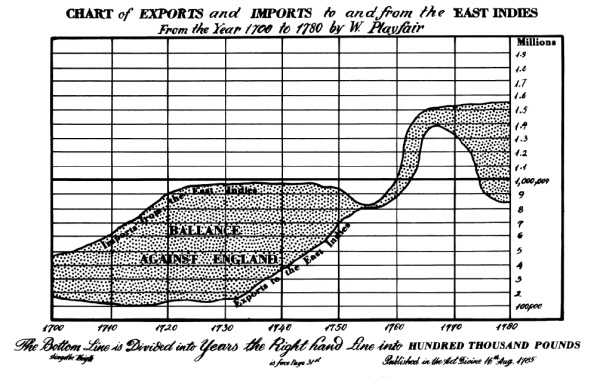
\includegraphics[keepaspectratio=TRUE,width=.7\textwidth]{PlayfairExportImports}
\caption[Imports to and Exports from the East Indies in the 1700s]{Playfair's graph of exports to and imports from the East Indies demonstrates that the line width illusion is not only found on sinusoidal curves but is present whenever the slope of the lines change dramatically. The increase in both imports and exports circa 1763 does not appear to portray as large of a deficit as that in 1710, even though they are of similar magnitude.}
\label{fig:playfair-debt}
\end{figure}

\subsection{Perceptual Explanations for the Sine Illusion}\label{perceptualexplanations}\hfill\newline
While not thoroughly examined in the sensation and perception literature, the sine illusion has been classified as part of a group of geometrical optical misperceptions  related to the M\"uller-Lyer illusion \citep{day:1991} or the Poggendorf illusion \citep{poggendorf}, which puts the illusion into the framework of context-based illusions. \citet{day:1991} suggest that the sine illusion occurs due to misapplication of perceptual experience with the three-dimensional world to a two-dimensional ``artificial" display of data.  

Experience with real-world objects suggests that the stimulus of figure~\ref{fig:original} is very similar to a slightly angled top view of the 3-dimensional figure of a strip or ribbon describing waves in a third dimension, such as e.g.~a road does on rolling hills. This is sketched out in figure~\ref{ribbon1}. Our experience suggests immediately that changes in the width of the road are unlikely and resolves the illusion. While figure~\ref{ribbon1} shows the line segments slightly angled towards each other, figure \ref{ribbon2} shows a variation of the same plot with a  vanishing point set further away from the viewer. This makes the line segments almost parallel to each other and therefore more closely resembles the sketch of figure~\ref{fig:original}, in which the sine illusion was originally presented.

%By treating the graph as a two-dimensional projection of a three-dimensional figure, the illusion disappears and the line widths seem once more to be constant.


% Figure \ref{fig:ribbon-illusion} shows a possible three-dimensional context for the classical sine illusion; two ribbons are shown at varying perspective strengths. \todo[inline]{OK, we need to slow down here, but I'm not sure how to say it. That's why I'm asking all these questions.}
% \todo[inline]{How do the perspective plots relate to the illusion - in words. I can see it, but we need to describe it in the text as well. }
% \todo[inline]{Does the 3d perspective resolve the illusion?}
% 
% \todo[inline]{What is the difference between the first and the second perspective plot?}
% The first appears more natural \todo[inline]{What do you mean by more 'natural'?}, but the second still appears three-dimensional \todo[inline]{Why?} and is much closer to the sine illusion stimuli \todo[inline]{Why is it closer?}  with added shading. 

\begin{figure}[h!tbp]\centering

\begin{subfigure}[t]{.49\textwidth}\centering
\includegraphics[width=\textwidth, keepaspectratio=TRUE, trim=0in 1.5in 0in 1.5in]{fig-ribbon-illusion1}
\caption{Perspective plot of sine illusion\label{ribbon1}}
\end{subfigure}
\begin{subfigure}[t]{.49\textwidth}\centering
\includegraphics[width=\textwidth, keepaspectratio=TRUE, trim=0in 1.5in 0in 1.5in]{fig-ribbon-illusion2}
\caption{Perspective plot, vanishing point near infinity.\label{ribbon2}}
\end{subfigure}
\caption[Three-dimensional origins of the sine illusion]{Two different perspective projections of the same data responsible for the sine illusion. The first projection angles the lines and appears more natural, but the second projection suggests that the lines do not need to be angled to create the same three-dimensional impression.\label{ribbon}}
\end{figure}




\begin{figure}
\centering
\includegraphics[width=.4\textwidth]{fig-originalgrid}
\caption[Contextual origins of the sine illusion]{\label{fig:original-grid} The sine illusion with two individual lines highlighted. Horizontal grid lines do not help  to resolve the illusion, even though they provide a clear basis for comparison of line lengths. Readers are much better at assessing the length of the two singled out line segments; they are equal.}
\end{figure}

Recreating the three-dimensional context of the sine illusion might resolve the distortion, even if increasing the dimensionality of a graph is generally not recommended \citep{tufte, cleveland:1984} (though \citet{spence:1990} suggests that in certain cases additional dimensions are not misleading). While creating a three-dimensional projection of two-dimensional data might counteract the illusion, the process of projecting the data accurately into a higher dimension is not simple. The projection that best resolves the illusion likely is highly subjective and influenced by choices of angle and color gradient for depth cues. As there is not a single three-dimensional projection that corresponds to the two-dimensional data, this approach would only produce further visual ambiguity.
%and would also lead to distortions and instability in the visual display. In particular, there does not seem to be an simple guideline for determining the projection angle or color gradient  to create the illusory depth to remove the optical illusion. 

%That is, the illusion breaks down if the visual heuristic is pre-empted by an attempt to view the graph as if it were three dimensional or if each piece is considered without the surrounding context. 
Further complicating the situation, the illusion itself is insidious -- we trust our vision implicitly, to the point that when we understand something, we say ``I see''. This trust in our visual perception is seldom called into question, for our perception is optimized for interaction with a three-dimensional world. Artificial two-dimensional situations (such as graphs and pictures) may accurately represent the data and still produce a misleading perceptual experience.

The contextual cues of the overall trend are critical to the sine illusion's effect;  the illusion  only  holds when a substantial portion of the graph is considered simultaneously, which triggers our innate ability of perceiving one whole rather than the individual parts it consists of (principle of grouping; \citet{wolfe2012sensation}).
%without regard to the perceptual mechanisms at play. 
Considering only two line segments at a time resolves the illusion. The bold lines in figure~\ref{fig:original-grid} are clearly of the same length.  Comparisons of individual line lengths is visually a fairly simple task, and is done with a relatively high accuracy \citep{cleveland:1984}. 
\citet{day:1991} contains a more thorough discussion of how much surrounding context is required for the illusion to persist. 
%The illusion arises when sufficient context is available to induce an ambiguously three-dimensional figure.

%\FloatBarrier
\subsection{Geometry of the Illusion}\hfill\newline
%We have previously alluded to the fact that the sine illusion depends on the change in the slope of the underlying function; what follows is a geometric explanation of why this occurs. 
%Our perceptual system is particularly well optimized for three dimensions; in figure~\ref{fig:original}  this leads us to perceive the  shortest line between the top and bottom curves as the distance between the curves, i.e. the {\it orthogonal} width,  rather than the vertical distance. 
In figure~\ref{fig:original} we have seen that the our preference in evaluating line width is to assess {\it orthogonal} width rather than the difference along the vertical axis. 
Figure~\ref{fig:OrthogonalWidth} demonstrates the change in orthogonal width as the slope of the line tangent to the graph of $f$ changes; these changes correspond to our perception of apparent line length. 

\begin{figure}[h!tbp]
\includegraphics[width=.9\textwidth, keepaspectratio=TRUE]{fig-transform-illustration}
\centering
\caption[Geometry of the sine illusion]{\label{fig:OrthogonalWidth} The sine illusion with lines orthogonal to the tangent line at $f(x)$. The perception that the vertical length changes with $f(x)$ corresponds to changes in actual orthogonal width due to the change in the visual (plotted) secant angle. The strength of the perceptual effect depends in part on the aspect ratio of the graph, as shown in the second image, which has an aspect ratio of 2 compared to the first figure's aspect ratio of 1. This correspondingly multiplies the strength of the effect by 2. 
}
\end{figure}
%Secants and vertical lines are both shown  in figure~\ref{fig:OrthogonalWidth}. 
The illusion is most pronounced in regions where the angle between the orthogonal  and the vertical line is large. Changes to the aspect ratio therefore have a major impact on the strength of the sine illusion. Any change that alleviates the difference between perceived width and the perpendicular width, such as banking to 45$^\circ$ \citep{cleveland:88}, will alleviate the effect but not completely overcome it. 
The perceived length of the vertical line changes with the angle of the line perpendicular to the slope of $\sin(x)$, suggesting that the sine illusion stems from a conflict between the visual system's perception of figure width and the mathematical judgement necessary to determine the length of the vertical lines. 



Our preference for assessing figure width based on the orthogonal width suggests that the underlying illusion may be a function of geometry rather than some unknown visual or neural process that occurs subconsciously. In this  case it may be  possible to correct the graphical display for the illusion to minimize its misleading effect. A geometrical correction that  --at least temporarily-- counteracts the illusion would be a valuable tool in visual analysis, as this illusion very persistently affects our judgment of very common tasks  such as e.g.~the assessment of conditional variability of data along a trend line.

Simply raising people's awareness of the presence of this illusion is not enough,
as it is incredibly difficult, if not impossible, to overcome this illusion even when we are aware of its presence: our brains simply cannot ``un-see" it. 

What follows is a compilation of several approaches to correct for or mitigate the effect of the illusion. Our primary intention here is to demonstrate the persaviness of the illusion is and the extreme measures necessary to remove its effect. 
% do not change this to its'

\section{Breaking the Illusion}
The sine  illusion is caused by a conflict between vertical width, which is the width that we want onlookers to assess visually, and orthogonal width, which is the width that the onlooker perceives. This difference can be expressed as a function in the slope of the underlying trend line. This provides the basis for adjusting the vertical width for the perceived orthogonal width. 

We consider the following three approaches:  
\begin{enumerate}
\item separating the trend and the variability, 
\item transformation of $x$: adjusting the slope to be constant by reparametrizing the $x$ axis, and
\item transformation of $y$: adjusting $y$ values to make conditional variability  appear correctly by adjusting accordingto orthogonal width. 
\end{enumerate}
Each of these ideas is discussed in more detail in this section.

\subsection{Trend Removal}
% \newdo{Emphasize that multiple plots imply higher cognitive load (Wainer 1984) and that good  charts usually have to answer multiple questions.}
\citet{cleveland:1984, cleveland:1985} discuss the perceptual difficulty of judging the difference between two curves plotted in the same chart, and alternatively, recommend to display the difference between the two curves directly. This is in line with  recommendations  for good graphics to `show the data' rather than make the reader derive some aspect of it (e.g. \citet{wainer:2000}). In particular, de-trending data to focus on residual structure is the generally accepted procedure for assessing model fit. 
 Figure \ref{fig:cleveland-figure}(a) shows a scatterplot of data with a trend. A loess smooth is used to estimate the trendline. A visual assessment of variability along this trendline
might result in a description such as `homogeneous variance or slightly increasing variance for  negative $x$, followed by a dramatic decrease in vertical variability for positive $x$'.  
Once the residuals are separated from the trendline as shown on the right hand side of the figure, it becomes apparent that this first assessment of conditional variability was not correct, and the decreasing variance along the horizontal axis becomes visible.
 
While the illusion is not apparent when trend line and variability in the  residual structure are shown separately, the separation 
makes it  more difficult to evaluate the overall  pattern in the data, as we  must base any judgment on two charts; either by combining information from two graphs or by mentally re-composing the original graph (at which point, the sine illusion becomes a factor). To minimize cognitive demands we ideally want to tell the whole story with a single graph, in particular because in many situations we may not be able to show multiple graphs. 


\begin{figure} \hfill
\begin{subfigure}[b]{.45\textwidth}
  \centering
  \includegraphics[width=\textwidth]{fig-cleveland1}
  \caption{\small Data}
  \label{fig:clevelandsubfig1}
\end{subfigure} \hfill\hfill
\begin{subfigure}[b]{.45\textwidth}
  \centering
  \includegraphics[width=\textwidth]{fig-cleveland2}
  \caption{\small Trend and Residuals}
  \label{fig:clevelandsubfig2}
\end{subfigure} \hfill
\caption[Changing variability and nonlinear trend lines]{Describe the conditional variability of the points along the $x$ axis in (a). Is your description consistent with the residual plot in (b)?}
\label{fig:cleveland-figure}
\end{figure}

%From a cognitive perspective, separating out the trendline and the variance creates a barrier to understanding the data in its original form; as the original graph must be mentally re-constructed.
Additionally, removing the trend requires an initial model, making any plots produced using that fit conditional on the assumptions necessary to obtain that model fit. In many situations, this may be undesireable. In particular, we typically view the data before fitting even a rudimentary model, and the sine illusion may influence even these initial modeling decisions.

\subsection{Transformation of the $X$-Axis}
As the sine illusion is driven by changes in the slope of trends between variables, we can counteract the illusion by removing these changes, transforming the $x$ axis such that the absolute value of the slope is constant and forcing the corresponding orthogonal width to represent the conditional variability.
In order to describe this transformation of the $x$ axis mathematically, 
let us assume that the relationship between variables $X$ and $Y$ is given by a  model of the form 
\[
y = f(x) + \varepsilon,
\]
where $f$ is some underlying function (either previously known or based on a model fit). Further let us assume that  $f$ is differentiable over the region of observed data.

Ideally, the correction would force all lines to appear under the same slope, i.e.~we want to find a transformation $T(x)$ of $x$, such that $f(T(x))$ is a  piece-wise linear function, where each piece has the same absolute slope. This transformation has an effect similar to ``banking to 45$^\circ$" in a piecewise manner. 

Let $a$ and $b$ be the minimum and maximum of the $x$-range under consideration. Then for any value $x \in (a,b)$ the following transformation results in a function with constant absolute slope:
\begin{equation}\label{eqn.xtrans}
(f \circ T)(x) = a + (b-a)\left(\int_{a}^x |f^\prime(z)| dz\right)/\left(\int_{a}^{b}|f^\prime(z)| dz\right),
\end{equation}

\subsubsection{Derivation of the X Transformation}\label{app.xtrans}
As the slope is determined by the aspect ratio, we are free to choose it and w.l.o.g. we get for each piece $T_i$: 
\[
f(T_i(x)) = \pm a x + b_i.
\]
This means that $T_i$ is essentially an inverse of function $f$, with each piece defined by the   intervals on which the inverse of $f$ exists: let $\left\{x_0 = \min(x), x_1, ..., x_{K-1}, x_K = \max(x) \right\}$ be the set of values with local extrema enhanced by the boundaries of the $x$-range, i.e.  $f^\prime(x_i) = 0$ for  $i = 1, ... , K-1$ and $f^\prime(x) \neq 0$ for any other values of $x$. 
Then each interval of the form $(x_{i-1}, x_i)$ defines one piece $T_i$ of the transformation function $T(x)$. We will define $T_i$ now as a combination of a linear scaling function and the inverse of $f$, which we know exists for interval $(x_{i-1}, x_i)$.

Let function $s = \s{[a,b]}{[c,d]}$ be the linear scaling function that maps  the interval $(a,b)$ linearly to the interval $(c,d)$. This function is formally defined as
\[
s(x) = \s{[a,b]}{[c,d]} (x) = (x-a)/(b-a) \cdot (d-c) + c \text{ for all } x \in (a,b).
\]
Note that the slope of function $s$ is given as
\[
s^\prime(x) = (d-c)/(b-a).
\]
%
Two scaling functions can be evaluated one after the other, only if the image (i.e. $y$-range) of the first coincides with the domain (i.e. $x$-range) of the second. This consecutive execution results in another linear scaling: 
\[
\s{[e,f]}{[c,d]}  \left(  \s{[a,b]}{[e,f]}(x) \right) = \s{[a,b]}{[c,d]} (x)
\]


In our situation let the scaling function $s$ be given as:
\[
\s{[c,d]}{f([x_{i-1}, x_i])}(x) = f(x_{i-1}) + (x-c)/(d-c) \cdot (f(x_{i}) - f(x_{i-1}))),
\]
where $f([x_{i-1}, x_i])$ is defined as the interval given by $(\min(f(x_{i-1}), f(x_i)), \max(f(x_{i-1}), f(x_i)))$.
Note that $s$ has either a positive or negative slope depending on whether $f(x_{i-1})$ is smaller or larger than $f(x_i)$, respectively.

Then the transformation in the $x$-axis, $T(x)$ is defined piecewise as a combination of $T_i$, where each $T_i$ is given as:
\begin{eqnarray}\label{eq.x.transformation}
T_i(x) &=& f^{-1}\left( \s{[c_i,d_i]}{f([x_{i-1}, x_i])}(x) \right). 
\end{eqnarray}
%
Using this definition for the transformation makes $f(T(x))$ a piece-wise linear function with parameters $c_i$ and $d_i$, i.e. for $x \in (c_i,d_i)$ we have
\[
f(T(x)) = f (f^{-1}(\s{[c_i,d_i]}{f([x_{i-1}, x_i])}(x))) = \s{[c_i,d_i]}{f([x_{i-1}, x_i])}(x).
\]
Correspondingly, the slope of $f(T_i(x))$ is $(f(x_{i}) - f(x_{i-1})))/(d_i-c_i)$.
In order to make the slope the same on all pieces $T_i$ of $T$, we need to define $c_i$ and $d_i$ with respect to the function values on the interval $(x_{i-1}, x_i)$. There are various options, depending on how closely the $x$-range of $T$ should reflect the original range:
for $[c_i, d_i] = \range {f([x_{i-1}, x_i])}$ the new $x$-range is the range of $f$ on $(x_{i-1}, x_i)$, but with the advantage that the scaling function simplifies to the identity or a simple shift.

In order to preserve the original $x$-range, we need to invest into a bit more work for the scaling. With an identity scaling, each $T_i$ maps from the range of $f$ on $(x_{i-1}, x_i)$ to the same range. Overall we can therefore set up the function $T$ to map from the interval given by the sum of the function's `ups' and `downs', i.e.
$(0, \sum_{i=0}^K |f(x_i) - f(x_{i-1})|)$, to the range of $f$ on $(x_0, x_K)$.  This ensures that all pieces $f(T_i)$ have the same slope (of $|1|$).We can then use another - global - linear scaling function to map from the range of $x$, i.e. interval $(x_0, x_K)$ to $(0, \sum_{i=0}^K |f(x_i) - f(x_{i-1})|)$, yielding a transformation function $T$ of

\[
T (x) =  (f^{-1} \circ \s{[c_i,d_i]}{f([x_{i-1}, x_i])} \circ \s{(x_0, x_K)}{(0, \sum_{i=0}^K |f(x_i) - f(x_{i-1})|)}) (x),  
\]
where $c_i$ and $d_i$ are given as 
\[
c_i = \sum_{j=0}^{i-1} |f(x_j) - f(x_{j-1})| \text{ and } d_i = \sum_{j=0}^{i} |f(x_j) - f(x_{j-1})|.
\]
We can write the difference $|f(x_j) - f(x_{j-1})|$ as $\int_{x_{j-1}}^{x_j} |f^\prime(z)|dz$. This shows equation (\ref{eqn.xtrans}).

\subsubsection{Weighting the X Transformation}
 As the sine illusion depends on changing slope in the overall trend,  re-parametrizing the $x$-axis in terms of the slope will make the data  appear under a  constant slope, thereby removing the effect of the illusion, while the transformed $x$-axis is changed from a linear representation of the $x$ values to a `warped' axis that continuously changes the scale of $x$ to compensate for the changes in the slope.
 To emphasize this change in scale along the $x$ axis,  dots are drawn at  the bottom of the chart  to show the transformation's effect on equally spaced points along the $x$-axis.   

Results from this transformation are demonstrated in Figure \ref{fig:xtrans1}.
 


\begin{figure}[h!tbp]\centering
\begin{subfigure}[b]{.45\textwidth}\centering 
\includegraphics[keepaspectratio=TRUE,width=\textwidth]{fig-xtransform1}
\caption[$X$ axis transformation]{$X$ axis transformation based on eqn.~(\ref{eqn.xtrans}), corresponding to weighting of $w=0$.}
\label{fig:xtrans1}
\end{subfigure} \hfill\hfill
\begin{subfigure}[b]{.45\textwidth}\centering
\includegraphics[keepaspectratio=TRUE,width=\textwidth]{fig-xtransform2} 
\caption[Weighted transformation]{Weighted Transformation, $w=1/2$ (based on eqn.~(\ref{eqn.xtrans.weighted}))}
\label{fig:xtrans2}
\end{subfigure}

\begin{subfigure}[b]{.45\textwidth}\centering 
\includegraphics[keepaspectratio=TRUE,width=\textwidth]{fig-xtransform3}
\caption[Weighted transformation]{Weighted Transformation, $w=1/3$}
\label{fig:xtrans3}
\end{subfigure} \hfill
\begin{subfigure}[b]{.45\textwidth}\centering
\includegraphics[keepaspectratio=TRUE,width=\textwidth]{fig-xtransform4}
\caption[Weighted transformation]{Weighted Transformation, $w=1/4$}
\label{fig:xtrans4}
\end{subfigure}
\caption[X axis transformations]{Examples of $X$ axis transformations in the sine curve.  Dots at the bottom of the graph show the transformation's effect on equally spaced points along the $x$-axis. Different amounts of weighting $w$ correspond to differently strong corrections. In (a),   $x$-spacing of the lines changes the extant width such that the absolute value of the slope is uniform across the whole range of the $x$ axis resulting in the largest amount of correction.  (b) - (d) reduce the correction in (a) towards successively more uniform spacings in $x$ while still breaking the effects of the illusion.}
\label{fig:xtrans}
\end{figure}
While the transformation in equation (\ref{eqn.xtrans}) effectively removes the appearance of changing line lengths, we can see in practice that the illusion can be broken by a much less severe transformation of the $x$ axis. 
For that we introduce a shrinkage factor $w \in (0,1)$ that allows a weighted approach in counteracting the illusion as: 
%
\begin{equation}\label{eqn.xtrans.weighted}
(f \circ T_w)(x) = (1-w) \cdot x + w \cdot (f \circ T)(x)
\end{equation}
%
Note that for $w=1$ the $x$-transformation is completely warped, while smaller values of $w$ indicate a less severe adjustment against the sine illusion.  Under  weaker transformations, the data more closely reflect the original function $f(x)$. 
Figures \ref{fig:xtrans2} - \ref{fig:xtrans4} show the effect of different shrinkage coefficients $w$. As $w$ decreases, the lines become more evenly spaced and the illusion begins to return. 

The extent  to which we can shrink the adjustment back to the original function  varies with the aspect ratio of the chart and the shape of the function. It might also be influenced by the audience's experience with the sine illusion, resulting in very subjective choices of an ``optimal weighting" for specific situations which minimizes distortion and maximizes the correspondence between inferences made from the data and inferences made using the visual display.


Note, that we only make use of the transformation $T$ in the form of $f \circ T$. This allows us to avoid an explicit calculation of the transformation $T$, which in particular  involves a computation of the inverse of $f$ leading to potentially computation-intense solutions. 
\subsubsection{X Transformation Demonstration}


In the example of the Ozone data shown in figure \ref{fig:exampleFull1}, we can base a transformation of the $x$-axis on a loess fit of ozone concentration in daily temperature. Loess is particularly convenient for this transformation, as it enforces continuity conditions including differentiability of the fitted function; software allows us to obtain fits of both the function values and their derivatives.

Figure \ref{fig:xtrans-example} shows the original data side-by-side with the transformed $x$-axis, demonstrating not only the effect of transformation of the $x$-axis, but also that the transformation is not overly misleading in this example. The granularity of the data in this example provides an implicit measure of the strength of the transformation along the $x$-axis and the transformation is also clearly evident in the labels along the $x$-axis. 
%
\begin{figure}[h!]\centering
\begin{subfigure}[b]{.48\textwidth}\centering
\includegraphics[keepaspectratio=TRUE,width=\textwidth]{fig-xtrans-example1}
\caption{Original Data}\label{fig:xtrans-example-original}
\end{subfigure}
\begin{subfigure}[b]{.48\textwidth}\centering
\includegraphics[keepaspectratio=TRUE,width=\textwidth]{fig-xtrans-example2}
\caption{Transformed $X$ Axis}\label{fig:xtrans-example-trans}
\end{subfigure}
\caption[Original data and data after X transformation]{Original data and data after $x$-transformation. The increasing variance is easier to see when $x$ has been transformed, because the slope is now uniform.\label{fig:xtrans-example}}
\end{figure}


\subsection{Transformation in $Y$}
Understanding the geometry of the sine illusion leads to another approach to counteracting  the conflict between the orthogonal width and the vertical length of the segment. 


Let again the function $f$ describe the general relationship between variables $X$ and $Y$. 


As sketched out in figure~\ref{fig:GeneralCorrection} we want to first find the orthogonal (extant) width in a point $(x_0, f(x_o))$ on the graph, which corresponds to the  perceived width, and then correct the vertical width accordingly to match with the audience's expectation.

\begin{figure}
\centering
\includegraphics[keepaspectratio=TRUE,width=.33\textwidth]{fig-generalcorrectioncartoon3}
\caption[General correction approach]{ General correction approach. This approach may require numerical optimization to obtain exact solutions for $(x_1, y_1)$ and $(x_2, y_2)$.}\label{fig:GeneralCorrection}
\end{figure}

The orthogonal width (see sketch in figure~\ref{fig:GeneralCorrection}) is given as the line segment between endpoints $(x_1, f_1(x_1))$ and $(x_2, f_2(x_2))$, where $f_1$ and $f_2$ denote the vertical shifts of function $f$ by $-\ell/2$ and $\ell/2$, respectively, where $\ell$ is defined as the overall line length, $\ell > 0, \ell \in \xR$.
These endpoints are determined as the intersection of the line  orthogonal to the tangent line in $(x, f(x))$ and the graphs resulting from the vertical shifts of $f$.

The function describing the orthogonal line through $(x_o, f(x_o))$ is given in point-vector form as 
\[
{x_o \choose f(x_o)} + \lambda {f^\prime(x_o) \choose 1}, 
\]
for any real-valued $\lambda$.
The advantage of using point vector form is that it allows us to solve for parameter $\lambda$ easily, which gives us easy access to the extant (half-)widths,  as: 
\begin{equation}\label{eqn.halfwidth}
|\lambda| \sqrt{1 + f^\prime(x_o)^2}.
\end{equation}
Eqn. (\ref{eqn.halfwidth}) describes the quantity that we perceive rather than the quantity that we want to display ($\ell/2$), which leads us to a general expression of the correction factor as
\begin{eqnarray*}
 \ell/2 \cdot \left(|\lambda| \sqrt{1 + f^\prime(x_o)^2}\right)^{-1}.
\end{eqnarray*}
Note that this yields in general two solutions: one for positive, one for negative values of $\lambda$ corresponding to upper and lower (half-)extant width.

In order to get  actual numeric values for $\lambda$, we need to find end points of the extant line width as solutions of intersecting the orthogonal line and  the graphs of $f_1$ and $f_2$. We find these end points  as solutions in $x$ and $\lambda$ of the system of equations:
\begin{eqnarray}\label{eqn.general}
 x - x_o &=& \lambda f^\prime(x_o)\\ \label{eqn.general.2}
 f(x) - f(x_o) &=& -\lambda \pm \ell/2
\end{eqnarray}


Note that  the above system of equations involves function values $f(x)$, which implies that solving this system  requires numerical optimization for any but the most simple functions $f$.

In the following two sections we make use of Taylor approximations of first and second order to find approximate solutions to end points as sketched out in figure \ref{fig:linear.quadratic}.




\begin{figure}[h!]\centering
\begin{subfigure}[t]{0.4\textwidth}\centering
\includegraphics[keepaspectratio=TRUE,width=0.9\textwidth]{fig-generalcorrectioncartoon2}
\caption{Linear Approximation}\label{fig:linear-GeneralCorrection}
\end{subfigure}
\begin{subfigure}[t]{0.4\textwidth}\centering
\includegraphics[keepaspectratio=TRUE,width=0.9\textwidth]{fig-generalcorrectioncartoon3}
\caption{Quadratic Approximation}\label{fig:quadratic-GeneralCorrection}
\end{subfigure}
\caption[Methods based on Approximations to f(x)]{(a) uses a first-order Taylor series approximation to $f(x)$ and (b) uses a second-order Taylor series approximation to $f(x)$. The intersection of the function $f(x) \pm \ell/2$ and the orthogonal line,  $(x_1, y_1), (x_2, y_2)$ must be obtained to determine the necessary correction factor.}\label{fig:linear.quadratic} 
\end{figure}

\subsubsection{Linear Approximation to $f(x)$}\hfill\newline
For the linear approximation we make use of $f(x) \approx f(x_0) + (x - x_0) f^\prime(x_0)$, which together with  equations~\ref{eqn.general} and \ref{eqn.general.2} yields a correction factor in $x_0$ of
\[
\ell_{\text{new}}(x_0) = \ell_{\text{old}} \sqrt{1 +  f^\prime(x_0)^2}.
\]

Note that the linear method gives the same result as a varying slope extension from a trigonometric approach  suggested by \citet{schonlau:2003} and used in \citet{parallelsets}.

A second-order Taylor polynomial approximation to $f(x)$ additionally accounts for the asymmetry in the extant widths on either side of the center trendline.

\subsubsection{Quadratic Approximation to $f(x)$}\hfill\newline
Using the approximation $f(x) \approx f(x_0) + f^\prime(x_0)(x-x_0) + 1/2 f^{\prime\prime}(x_0)(x-x_0)^2$, the system of equations~\ref{eqn.general} and~\ref{eqn.general.2}  simplifies to the following  quadratic equation in $\lambda$:
\begin{eqnarray*}
f^{\prime\prime}(x_0)  f^\prime(x_0)^2 \lambda^2  + 2(f^\prime(x_0)^2 + 1) \lambda  \pm \ell = 0,
\end{eqnarray*}
which leads us to corrections for the half lengths as:
\begin{eqnarray}\label{eqn.q1}
\ell_{\text{new}_1}(x_0) &=& 1 /2 \cdot  \left(v + \sqrt{ v^2 +  f^{\prime\prime}(x_0) f^\prime(x_0)^2\cdot  \ell_{\text{old}}}\right) \cdot v^{-1/2} \\\label{eqn.q2}
\ell_{\text{new}_2}(x_0) &=& 1 /2 \cdot  \left(v + \sqrt{ v^2 -  f^{\prime\prime}(x_0) f^\prime(x_0)^2\cdot  \ell_{\text{old}}}\right) \cdot v^{-1/2} 
\end{eqnarray}
where $v = 1 + f^\prime(x_0)^2$.

\begin{subsubsection}{Reformulation of the quadratic approximation}\label{app.quadratic}
A quadratic equation in $\lambda$ of the form 
\begin{equation}\label{quadratic.equation}
a\lambda^2 + b\lambda + c = 0,
\end{equation}
where $a, b,$ and $c$ are real-valued parameters the solutions take on the form
\begin{eqnarray*}
\lambda_{\pm} = \frac{-b \pm \sqrt{b^2 - 4ac}}{2a}
\stackrel{*}{=} 2c\left(-b \pm \sqrt{b^2 - 4ac}\right)^{-1}.\\
^*\text{ if } b \neq \pm &\sqrt{b^2 - 4ac}\text{, i.~e. }a, c \neq 0.
\end{eqnarray*}

\paragraph{Application to quadratic approximation to $f$:}
in the example, we have the following equivalencies:
\begin{eqnarray*}
a &=& f^{\prime\prime}(x_0) f^\prime(x_0)^2 \\
b &=& 2(1 + f^\prime(x_0)^2) \hspace{.5in} > 0 \text{ for all } x \\
c &=& \pm \ell 
\end{eqnarray*}
For a valid solution for the correction factor, we have to assume that $\lambda$ is a factor that extends the original extant width (in absolute value). 

\begin{eqnarray*}
\lambda_{1/2} &=& \ell \left(v + \sqrt{ v^2 \pm  f^{\prime\prime}(x_0) f^\prime(x_0)^2\cdot \ell}\right)^{-1} 
\end{eqnarray*}
for $v = 1 + f^\prime(x_0)$. 
This gives the results as shown in equations (\ref{eqn.q1}) and (\ref{eqn.q2})
\end{subsubsection}

\begin{figure}
\begin{subfigure}[b]{.32\textwidth}\centering
\begin{knitrout}
\definecolor{shadecolor}{rgb}{0.969, 0.969, 0.969}\color{fgcolor}

{\centering \includegraphics[width=\textwidth]{../Figure/sineIllusion/fig-UncorRresults-1} 

}



\end{knitrout}
\caption{Uncorrected}
\end{subfigure}
\begin{subfigure}[b]{.32\textwidth}\centering
\begin{knitrout}
\definecolor{shadecolor}{rgb}{0.969, 0.969, 0.969}\color{fgcolor}

{\centering \includegraphics[width=\textwidth]{../Figure/sineIllusion/fig-LinearResults-1} 

}



\end{knitrout}
\caption{Linear correction}
\end{subfigure}
\begin{subfigure}[b]{.32\textwidth}\centering
\begin{knitrout}
\definecolor{shadecolor}{rgb}{0.969, 0.969, 0.969}\color{fgcolor}

{\centering \includegraphics[width=\textwidth]{../Figure/sineIllusion/fig-CtsAdjustedResults-1} 

}



\end{knitrout}
\caption{Quadratic correction}
\end{subfigure}
\caption[Quadratic Approximation]{
In the quadratic approximation top and bottom segments of the vertical lines are adjusted separately.}
\label{fig:GeneralQuadraticCorrection} 
\end{figure}

Adjusting the top and bottom segments of the vertical lines separately so that the extant width is constant breaks the illusion, but slightly distorts the sinusoidal shape of the peaks.

Figure~\ref{fig:GeneralQuadraticCorrection} shows the correction factor based on a quadratic approximation compared to the untransformed data. 
Unlike the linear solution, the half-segments here are not necessarily of the same length, and thus there are separate correction factors for each half-segment. 


\subsubsection{Mathematical Properties of the Y Transformation}
The quadratic correction breaks whenever the expression in the square root of eqn.~(\ref{eqn.q1}) becomes negative, i.e.~whenever $v^2 \pm \ell\cdot f^{\prime\prime}(x)\cdot f^\prime(x)^2 < 0$.
This happens for  combinations of large values of $\ell$, which signify a large vertical extent, or large conditional variability $E[Y|X]$, and simultaneous large changes in the slope of the main trend, i.e.~large values of the curvature $f^{\prime\prime}(x)$. In the linear approximation of $f$ the same situation leads to a massive overcorrection of the vertical lines, changing the shape of the `corrected' function beyond recognition.

Similar to the correction of the $x$-axis,  we can use a weighted approach to find a balance between counteracting the illusion and representating the  original data:
\begin{equation}\label{eqn.ytrans.weighted}
\ell_{new_w}(x) = (1-w) \cdot \ell_{old} + w \cdot \ell_{new}(x)
\end{equation}

\section{Transformations in Practice -- a User Study}

In order to more fully understand the sine illusion and test the proposed corrections, we created an applet to allow users to investigate the illusion's prominence with respect to its parameters. Users can examine the sine illusion by changing line length, the function's amplitude, and compare corrections in $x$-axis and $y$-values to uncorrected data.  All corrections proposed in this paper are  implemented in the applet located at \url{http://glimmer.rstudio.com/srvanderplas/SineIllusion/}.

We employed a second applet to collect data on users' preferences on the amount of correction used, i.e.~we are interested in identifying a range of `optimal weights' in each of the corrections. This applet presents users with a graph that is the result of a correction in $x$ or $y$ with a randomly selected starting weight value. Users are asked to adjust the graph until the illusion  (a) is no longer apparent (adjustment of weights from the bottom) or (b) becomes visible (adjustments of weights from the top).

Both applets are implemented in {\tt shiny} \citep{shiny}. 

The graphs in the data-collection applet are adjusted using a plus/minus button to either increase or decrease the amount of correction used. Underlying this adjustment is the value of the weight $w$ as defined in eqns.~(\ref{eqn.xtrans.weighted}) and~(\ref{eqn.ytrans.weighted}). The numerical value of $w$ was hidden from the user to prevent anchoring to a specific numerical value.

A low  initial weight ($w_0$ close to 0) indicates that the amount of correction is low and the response from a trial like this will give us an idea of the minimal amount of weight necessary to break the illusion, while a high initial weight ($w_0$ close to 1) indicates that the data is fully corrected. We asked participants to change the amount of adjustment until the lines appear to be the same length assumes that the correction is overcorrecting in practice, and a response from this type of trial gives us an upper boundary for the amount of weighting preferred. Generally, responses from the two different types of trials do not result in the same threshold weight, but rather lead to a range of acceptable weights.

It is of additional interest to determine whether and how much these optimal weights are subject-specific or population-based, whether they depend on the initial weight, and how much within-subject variability we find compared to between-subject variability. 

\begin{figure}\centering
\includegraphics[width=.92\textwidth]{shiny}
\caption[Screenshot of Data Collection Website]{\label{fig:shiny.app} Screenshot of the shiny application used to collect information of observers' preference with respect to an optimal correction for the illusion under each of the  transformations discussed in the previous section. }
\end{figure}

Figure~\ref{fig:shiny.app} shows a screenshot of the applet used to collect user data. This applet is  available online at \url{http://glimmer.rstudio.com/srvanderplas/SineIllusionShiny/}. 
Line length and function are controlled in this app, and we used the linear transformation for adjusting $y$ values; the transformation does not break under any combination of parameters tested in this experiment. 


\noindent
We deployed the applet to participants recruited online, collecting their responses and other metadata. The results of the analysis suggest that the correction factors in $X$ and $Y$ are both preferrable to uncorrected data, but that a full correction is not necessary to break the illusion.



\subsection{Study Design}
The study aims to determine the range of ``optimal'' transformation weights for each transformation type. Psychophysics methodology typically approaches threshold estimation by using the method of adjustment \citep{goldstein}, where  stimuli are provided showing states both above and below the hypothesized optimal value and  participants adjust the stimuli until the stated goal is met (in this case, until the lines appear to have equal length). It is expected that there will be a difference in user-reported values from below and from above, and these values are typically averaged to produce a single threshold value. Beyond averaging these values, we use a mixed model to compare user responses for different starting points in a more continuous fashion, incorporating some of the advantages of the method of constant stimuli to more robustly estimate the range of optimal transformation weights. For a review of general psychophysics methodology, the method of adjustment, and the method of constant stimuli, see \citet{goldstein}.

The study is set up as a fractional factorial design of correction type ($x$ or $y$ correction) and starting weight $w_0$. Each participant is asked to evaluate a total of twelve situations, six of each correction type.
Starting weights were chosen as follows: each user was given a trial of each type starting at 0 and 1. The remaining four trials of each type had starting weights chosen with equal probability from $0.25$ to $0.75$ 
(see figure~\ref{fig:weightdist}). 
We decided to  have a higher coverage density for starting weights around 0.6 after a pilot study indicated a preference for that value. Using a distribution with a wide coverage allows us to more fully explore the space of plausible weights $w$ while focusing on the $(0,1)$ interval and enabling precise estimation of the optimal weight in the region indicated by the pilot study.

\begin{figure}\centering
\includegraphics[keepaspectratio=TRUE,width=0.8\textwidth]{fig-study-weight-dist}
\caption[Overview of possible starting weights]{Overview of possible starting weights. Weight values are discrete, but staggered so as to provide fine-grained adjustments around 0.6 and more coarse discriminatory information toward the outside.}\label{fig:weightdist}
\end{figure}

A trial begins with the presentation of a graph at the chosen starting weight $w_0$. Participants adjust the graph using increment and decrement buttons. A trial ends with the participant clicking the `submit' button, at which point the weight for the final adjustment is recorded. This provides a clear starting value and ending value, allowing us to assess the range of optimal values for each participant. In addition to starting weight, correction type, and anonymized user-specific data (partial IP address, hashed IP address, and hashed browser characteristics), each incremental user chosen weight is recorded with a corresponding timestamp. The user-specific browser data is sufficient to provide a `fingerprint' to distinguish and recognize individual users (or rather their computer settings) in an anonymous fashion. 

Each participant is provided with two initial ``training'' trials in which the  graph of the underlying mean function is superimposed on the line segments to give participants some idea of the  function the lines represent. This approach was taken to reduce  incidences of extremely high  correction values under the $X$ transformation, as large adjustment values do not change the impression of same line length, but the resulting function bears little resemblance to a sine function, see figure~\ref{fig:overtransform} for examples of overcorrection.




\begin{figure}\centering
\includegraphics[keepaspectratio=TRUE,width=.8\textwidth]{fig-overcorrectlimits}
\caption[ Overcorrected transformations excluded from the analysis]{Transformation weights outside of the intervals $[\ensuremath{-2.5}, 3.5]$ for $y$ and $[\ensuremath{-2}, 2]$ for $x$  produce figures which do not maintain the underlying function shape (in $x$) or which are composed of extremely uneven length lines (in $y$). Trials with final results that were more extreme than these examples were excluded from the analysis.}
\label{fig:overtransform}
\end{figure}

\subsection{Results}

Participants were recruited from Amazon Mechanical Turk and the \href{http://reddit.com/r/SampleSize}{reddit} community.

As this study was conducted outside a laboratory setting, we can not gauge a participant's willingness to follow the guidelines and put in their best effort. This, besides potential technical issues (server outage, speed of response) make a careful selection of data going into the analysis unavoidable. The following exclusion criteria were used:
\begin{itemize}
\item Participants did not interact with the applet: we required participants to use the adjustment at least once in order to include data for this trial (592 trials removed).
\item Participants finished fewer than four trials: while participants were asked to complete twelve trials, some did not finish all of those. In order to stabilize predictions of random effects, participants' data were excluded if there were fewer than four trials (78 out of a total of 203 participants).
\item Out-of-bounds results: weights leading to severely over- or undercorrected results were excluded from the analysis. 
For trials to adjust $Y$-values, weights outside of [\ensuremath{-2.5}, 3.5]  show dramatically unequal line lengths; weights from $X$-transformations outside the range of [\ensuremath{-2}, 2] do not preserve the underlying function shape and concavity. 
Figure~\ref{fig:overtransform} shows results at the threshold of acceptability. Only more severely distorted results were excluded from the analysis (12 of the $X$ and 5 of the $Y$ trials out of 1227 trials remaining after application of other criteria).
\end{itemize}


The following analysis is based on the cleaned data, consisting of 125 participants with 1210 valid trial results. The psychophysics model shown in figure \ref{fig:psycho} is based on  weighted averages (by adjustment type) of all trials with starting weights $w_0 = 0$ and 1.


\begin{figure}\centering
\begin{knitrout}
\definecolor{shadecolor}{rgb}{0.969, 0.969, 0.969}\color{fgcolor}

{\centering \includegraphics[width=.5\textwidth]{../Figure/sineIllusion/fig-meanDists-1} 

}



\end{knitrout}
\caption[Results from psychophysics analysis]{Estimated density of participant-level means using the standard psychophysics method of limits analysis. The overall means are both near 0.4, however, there is quite a bit of user-level variability.\label{fig:psycho}}
\end{figure}



According to this analysis, the optimum transformation value for $x$ is 0.35, and the optimum transformation value for $y$ is 0.45. Figure \ref{fig:psycho} shows the estimates and 95\% Wald intervals for the mean, as well as estimated density of participant-level responses. 

While these results suggest that the transformation is useful and that complete transformation is not necessary, we can get more precise bounds on the range of acceptable transformation weights using a linear model that can incorporate starting points other than 0 and 1, and at the same time allow for user-specific variability.

In order to account for user-level variability, we fit a random effects model for the adjusted weight value as a function of  starting weight and trial type, with a random intercept for each participant. 

Let $W_{ij}$ denote the final adjustment to weight by participant $i$, $ 1 \le i \le 125$ , on trial $j$, $1 \le j \le n_i$. 
We model the final weight $W_{ij}$ as a function of the correction type $T(i,j)$  (where $T(i,j) \in  \{X, Y\}$), and starting weight $X_{ij}$, with a random intercept for participant to account for subject-specific ability: 
\begin{align}\label{model1}
W_{ij} &= \alpha_{T(i,j)} + \beta X_{ij} + \gamma_{i, T(i,j)} + \epsilon_{ij}\\
& \gamma_{iX} \stackrel{\text{ i.i.d.}}{\sim} N(0, \eta_X^2) , \ \gamma_{iY} \stackrel{\text{ i.i.d.}}{\sim} N(0, \eta_Y^2) ,\notag  \\
& \epsilon_{ij} \stackrel{\text{ i.i.d.}}{\sim} N(0, \sigma^2)  \text{ and } \text{Cov}(\gamma, \epsilon) = 0\notag 
\end{align}
 $\alpha_{T(i,j)}$ is either $\alpha_X$ or $\alpha_Y$, describing the lower threshold of the acceptable range for each of the types of correction, while $\alpha_X+\beta$ and $\alpha_Y + \beta$ describe the upper thresholds for the respective correction.

We can therefore interpret $\beta$ as the length of the interval of plausible weights. Additionally, this allows the interpretation of the quantity $(\alpha_* + \beta/2)$ as equivalent to the estimate of the optimal weight based on the psychophysics methodology.

\noindent
The fitted model parameters are shown in tables \ref{fixedeffectsresults} and \ref{randomeffectsresults}. 


\begin{table}[htbp]\centering
\begin{tabular}{cclcc}
  \hline
Transformation & Threshold &  \multicolumn{1}{c}{Parameter} & Estimate & 95\% C.I. \\ 
  \hline
X & Lower & $\alpha_X$ & 0.097 & (0.045, 0.150) \\ 
   & Upper& $\alpha_X + \beta$  & 0.625 & (0.570, 0.682) \\ 
  Y & Lower& $\alpha_Y$  & 0.143 & (0.097, 0.188) \\ 
   & Upper& $\alpha_Y + \beta$  & 0.671 & (0.626, 0.718) \\ 
   \hline
\end{tabular}
\caption[Sine Illusion Model: Fixed Effects]{Fixed effect estimates of model~(\ref{model1}) for the boundaries for reasonable weights. In parentheses,  95\% parametric bootstrap confidence intervals are given based on model (\ref{model1}) ($N$=1000).}\label{fixedeffectsresults}
\end{table}
\begin{table}[hbtp]\centering
\begin{tabular}{rcccc}
  \hline
Groups & Correction & Parameter & Estimate & 95\% C.I. \\ 
  \hline
  Participant & X &$\eta_X$  & 0.171 & (0.167, 0.247) \\ 
  Participant & Y &$\eta_Y$ &  0.145 & (0.107, 0.179) \\ 
  Residual &  &$\sigma$ &  0.304 & (0.290, 0.317) \\ 
   \hline
\end{tabular}
\caption[Sine Illusion Model: Random Effects]{Overview of random effects for model~(\ref{model1}), including 95\% confidence intervals based on parameteric boostrap results ($N$=1000).}\label{randomeffectsresults}
\end{table}

Table \ref{randomeffectsresults} gives an overview of the variance estimates. 95\% confidence intervals are, based on 1000-fold parametric bootstrap of model~\ref{model1}. All variance components are significant and relevant; variability within a single individual's trials is about half the size of variability across  participants. 

We use parametric bootstrap to generate responses for each correction type and each participant from the model, which we use to both  create user-level densities, population-level densities, and bootstrap intervals for model parameters. 


The variability of the random effects for each trial type is similar; but the model benefits significantly from allowing separate random effects for individual's variability by correction type (0.1452402 and 0.1705484 for $Y$ and $X$ transformations, respectively, as opposed to 0.3044343 for the overall variability). The interaction between starting weight and trial type was not significant, however, and was thus removed from the model ($p$-value = 0.9009749).

\begin{figure}[hbtp]
\centering
\includegraphics[keepaspectratio=TRUE, width=.85\textwidth]{fig-results-analysis1}
\caption[Results from mixed model]{Simulation results from the fitted model, facetted by correction type. Fixed effects results are shown as histograms; the red values display the results when starting from an uncorrected plot and are concentrated around $w=0.1$ for $X$ and $w=0.14$ for $Y$; the blue values represent user-chosen weights when starting from a fully corrected plot and are concentrated around $w=0.63$ for $X$ and $w=0.67$ for $Y$. Additionally, 95\% bootstrap intervals are shown as horizontal line segments above the histograms; these intervals are for the lower and upper bounds of the ``preferred weight interval" tested in the experiment. User-level density curves show the individual variability around  fixed effects $\alpha_*$ and $\alpha_*+\beta$.}\label{fig:MixedModelResults}
\end{figure}
Figure \ref{fig:MixedModelResults} gives an overview of the relationship between starting weights and  user-preferred weight values. Higher starting weights are associated with higher user-submitted values, and lower starting weights are associated with lower user-submitted values.

The ranges of optimal weights are similar under both transformations. Boundaries for the $X$ transformation are slightly lower than boundaries for $Y$. 

Bootstrap simulations for each of the coefficients suggest that the range of optimal $w$ is between 0.098 and 0.625 for $x$ and 0.142 and 0.67 for $y$, where the lower value is the estimate starting at $w=0$ and moving up, and the upper value is the estimate starting at $w=1$ and moving down. This suggests that either correction is preferrable to an uncorrected graph, and that a weighted correction is preferrable to the fully corrected graph, as neither 0 nor 1 is contained in any overall interval. In addition to showing the strength of the correction, this experiment also demonstrates the strength of the illusion itself: a correction appears more uniform than the uncorrected values, even though the corrected values are not uniform and the uncorrected values are completely uniform. 

\section{Application: US Gas Prices}
Figure~\ref{fig:gasprices} shows daily gas prices for a time frame between 1995 to 2014 as published in the Energy Information Administration's historical database of gas prices \citep{EIA}. This data includes prices for all three grades of gasoline as well as two chemical formulations which are sold in different geographic areas across the United States (for more information, see \citep{EIA-reformulated}). 

\begin{figure}[h!tbp]
\begin{knitrout}
\definecolor{shadecolor}{rgb}{0.969, 0.969, 0.969}\color{fgcolor}

{\centering \includegraphics[width=.98\textwidth]{../Figure/sineIllusion/fig-gasprices-pictures-1} 

}



\end{knitrout}
\caption[US Gas prices from 1995 to 2014]{US Gas prices from 1995 to 2014. Gas prices steadily increase over the time frame, with some dramatic short-term developments. Peaks and troughs seem to exhibit more variability in daily prices than times of dramatic changes. This is an effect of the sine-illusion, which hides a fairly steady increase in variance in daily gas prices over time.}\label{fig:gasprices}
\end{figure}
\begin{figure}\centering
\begin{knitrout}
\definecolor{shadecolor}{rgb}{0.969, 0.969, 0.969}\color{fgcolor}

{\centering \includegraphics[width=.7\textwidth]{../Figure/sineIllusion/fig-gaspricevariance-1} 

}



\end{knitrout}
\caption[Standard deviation of daily gas prices between 1995 and 2014. ]{Standard deviation of daily gas prices between 1995 and 2014. The doubling of the standard deviation over the time frame is masked in figure \ref{fig:gasprices}.\label{fig:gasvariance}}
\end{figure}
There is a clear increase in daily gas prices over time as well as several dramatic price changes. These developments mask the steady increase in variance shown in figure~\ref{fig:gasvariance}. Instead, we perceive an increase in variability in the frequent ups and downs along the overall trend. In particular, the strong decrease in gas prices at the end of 2008 seems to be associated with a low variance. This is an effect of the sine illusion, and the actual variability in Oct 2008 is higher than previous months. In order to better judge variability along the trendline we applied the two different corrections to this data. 

For either of the corrections we use a trendline fit based on smoothing splines, which provides the necessary first and second derivatives.




Figure \ref{fig:gasprices-x-correct} shows the results from the $X$ transformation applied to the gas prices. The figure on top is a fully corrected version, while the one below only uses $w=0.36$, the midpoint of the range of experimentally determined acceptable values,  for the transformation. At $w=1$, the transformation is severe, but it becomes clear that the variance between 1995 and 2000 is lower than it is between 2009 and 2014. When $w=0.36$, the transformation is much less noticable but yields a near-constant absolute slope of the fitted line.

\begin{figure}
\centering
\includegraphics[keepaspectratio=TRUE,width=.92\textwidth]{gas-x-corrected}
\caption[Gas price data, X transformation]{Gas price data corrected using the $X$ transformation with $w=1$ and with $w=0.36$. }
\label{fig:gasprices-x-correct}
\end{figure}
The minor effect of the weighted transformation on individual x-values contrasts with the effectiveness of the transformation in reducing the illusion; this is best seen in the fitted line, which is distinctly (piecewise) curved in the uncorrected data and appears to be much more piecewise linear in the corrected data, even at the reduced weighted value. 

Similar to the $X$ transformation, the $Y$ transformation highlights local fluctuation in the variability of daily gas prices much more than the untransformed data. Figure~\ref{fig:gasprices-y-correct} shows $Y$ transformations for the data. Again, we show a full transformation (top) and a transformation based on the midpoint of the previously determined acceptable region of $w=0.40$.
in the full transformation  it is clear that the variance is nearly constant between 1995 and 2000 and then begins to increase with the price of gas. When $w=0.40$, the transformation is much less noticable, and the resulting $y$-axis scale is much more similar to the uncorrected data. 

\begin{figure}[h]
\centering
\includegraphics[keepaspectratio=TRUE,width=.92\textwidth]{gas-y-corrected}
\caption[Gas price data, Y transformation]{Gas price data corrected using the $Y$ transformation with $w=1$ and with $w=0.40$. }
\label{fig:gasprices-y-correct}
\end{figure}

\section{Conclusions}
The sine illusion is a persistent and powerful illusion that is very difficult to counteract without modifying the visual stimulus directly. While systematically modifying the data is uncommon in the statistical world, this approach is not out of place in the visual arts or architecture; as far back as 400 BC the builders of the Parthenon ensured a straight appearance of the columns from afar, by widening columns at the center, thereby counteracting the effects of the Hering illusion \citep{naturalscenes,hering}. Similarly, painters often exaggerate color hues used in shadows to account for color constancy in the brain. The systematic modifications we suggest here are also comparable to chloropleth maps, which scale a region's area based on some other variable. 

We cannot counteract the illusion and represent the data visually without an intervention that is drastic enough to counteract the three-dimensional context the sine-illusion induces. The proposals in this paper for transformations in $x$ and $y$ provide the means to temporarily correct the data as a diagnostic measure, perhaps using an applet or R package for that purpose. These corrections are significant not only because of their implications for statistical graphics, but because previous attempts to resolve optical illusions using geometry have not met with success \citep{westheimer2008illusions}. These corrections are only a first step and could be improved upon; currently, the corrections break down for extreme (secant) values, but multiple iterations of the correction procedure will likely resolve some of these issues (though iteration removes the convenience of a functional form for the transformation). Similarly, the $y$ corrections proposed here extend the line lengths (or for actual data, increase the deviation from the smooth line) -- some normalization might make the necessary corrections less noticeable. 

Our primary goal is to raise awareness of the illusion and its implications for statistics; the use of plots to guide the modeling process can leave us vulnerable to overlooking changes in the variance due to the illusion. While best practice has  been to plot the residuals separately, this removes the context of the data and is not practical before there is a model. In addition, viewer attention spans may be limited if multiple graphs are presented. The proposed transformations require only a nonparametric smooth, maintain the context of the data, and are readily interpretable. 

The data for this study was collected with approval from  IRB-ID 13-257.



\graphicspath{{Figure/lieFactorSine/}{Images/lieFactorSine/}}
\renewcommand{\floatpagefraction}{.99}
% 
% \newcommand{\range}[1]{{\text{range}\left(#1\right)}}
% \newcommand{\s}[2]{{_{#1}s^{ #2}}}
% \newcommand{\atan}[1]{\text{atan}\left({#1}\right)}
% \newcommand{\xR}{\mathbb{R}}
% 





\chapter{THE CURSE OF THREE DIMENSIONS: WHY YOUR BRAIN IS LYING TO YOU}\label{LieFactorChapter}\label{liefactor}
%% Abstract
% One of the basic principles of information graphics is that the data should be accurately reflected in the chart. Tufte's lie factor was created with the idea that graphs that do not represent the underlying data accurately should be avoided. In this paper, we examine a second level of graph distortion that occurs during the perceptual process. The human visual system is largely optimized for perception of three dimensions. Generally, the brain processes potential  ambiguities in the rendering as the most-common three-dimensional object. This can lead to visual distortions, such as occur with the Necker figure or in the M\"uller-Lyer illusion. We discuss the underlying psychological mechanisms for the distortions, examine the effect these distortions have on  judgments, and consider the implications for graph design. Using the sine illusion as a case study, we quantify the effects of the distortion that create a ``perceptual lie factor" for the sine illusion.


\section{Introduction}
Graphics are one of the most powerful tools researchers have to communicate results to wide audiences. They are easier to understand than tables or verbal descriptions\citep{larkin1987diagram}, easier to remember than words alone \citep{mayer1994whom}, and provide information that can be perceived and used with minimal additional cognitive load \citep{zhang1994representations}. Conveying numerical relationships using spatial information makes use of the brain's visual processing ability, freeing working memory to interpret and make connections between graphics and written interpretations. Informative graphics differ from visualizations, sketches, and diagrams in that they present visual summaries of data, using summary functions to map the data graphically, preserving the relationship between two variables using spatial information. That is, unlike visualizations, sketches, and diagrams, spatial relationships presented in information graphics are functions of the data, representing numerical quantities (within the limits of image resolution) accurately. 

In fact, the primary principle of informative graphics is that a chart should accurately reflect the data \citep{tufte}. Tufte argues that some graphics (many of which might be better classified as visualizations) do not accurately reflect the data because they blend artistic rendering with numerical information, sacrificing numerical accuracy for visual appeal. In order to quantify the loss of numerical accuracy, Tufte created the lie factor, which compares the effect size shown in the image to the effect size shown in the data, so that a lie factor much greater than 1 indicates a picture that over-emphasizes an effect, and a lie factor much smaller than one indicates a picture which minimizes an effect (values between .95 and 1.05 are typically acceptable). While Tufte's lie factor is an effective measurement of the accuracy of the transition from data to graphics, it does not give us any insight about the transition between a chart and the brain, that is, whether the mental representation of the chart is accurate.

Ideally, charts not only represent the data accurately, but  also allow readers to draw accurate conclusions. Generally, the human visual system is quite good at accurately interpreting charts \citep{cleveland:1984,kosara2010}, but we need to be aware of contextual misperceptions that lead us to the wrong conclusion. While there are relatively few examples of the effect of optical illusions and other misperceptions on information graphics, \citet{amer2005bias} and \citet{poulton1985geometric} have documented the effect of the Poggendorff illusion on line graphs in different contexts. In this paper, we examine a situation in which low-level human perceptual processes interfere with making accurate judgements from displays and suggest an experimental methodology for estimating the psychological ``lie factor" of a chart due to a specific conceptual misperception: the sine illusion. 

\subsection{The Curse of Three Dimensions}
The human visual system is largely optimized for perception of three dimensions. Biologically, binocular vision ensures that we have the necessary information to construct a functional mental representation of the three-dimensional world, but even in the absence of binocular information the brain uses numerous heuristics to parse otherwise ambiguous two-dimensional retinal images into meaningful three-dimensional information. Predictably, however, these heuristics are not without drawbacks; the same two-dimensional neural representation might correspond to multiple three-dimensional objects, as in the well-known Necker Cube (\citet{gregory1968perceptual}; shown in figure~\ref{fig:Necker}). Additionally, the same three-dimensional object often has infinitely many two-dimensional representations, for instance, when viewed from different angles. 
Many optical illusions occur due to the transition from a two to three dimensions (or from three dimensions to two dimensions)\citep{gregory1968perceptual}. The necker cube has a single two-dimensional representation corresponding to two three-dimensional objects which are both equally salient. As a result, the brain does not prefer one interpretation over the other and instead continuously switches between interpretations.
Impossible objects, such as the Penrose triangle \citep{penrose1958impossible}, are two-dimensional images of objects that appear to be impossible in three dimensions (sometimes, these objects can be represented in three dimensions, but only appear to be impossible from a certain angle). Impossible objects produce a conflict between the brain's three-dimensional representation of a two-dimensional figure and the brain's experience with the physical world. This conflict between the constraints of physical reality and a depicted image can be quite compelling and is an important component in the work of artists like M.C. Escher \citep{Escher}.

\begin{figure}
\includegraphics[keepaspectratio=TRUE,width=6in, trim=0in .25in 0in 0in]{fig-neckercube}
\caption[Necker Cube]{The Necker Cube is a so-called ``ambiguous object" because two different transparent objects  produce the same retinal image (and thus the same perceptual experience). Commonly, the image seems to transition instantaneously from one possible mental representation to the other.}\label{fig:Necker} 
\end{figure}

In non-illusory contexts, experience with the real world informs the choice between multiple possibilities of rendering a three-dimensional object from the same two-dimensional representation. This indicates that processing occurs ``top down" in that our previous experience influences our current perceptions. Without this top-down influence, the brain would not be able to map a two-dimensional image back to a three-dimensional object. One of the most well studied examples of the influence of top-down processing is the M\"uller-Lyer illusion, shown in figure~\ref{fig:mullerlyer}.

\begin{figure}\centering
\includegraphics[keepaspectratio=TRUE, trim=0in .3in 0in .3in]{fig-mullerlyer}
\caption[The M\"uller-Lyer illusion]{The M\"uller-Lyer illusion. The central segment of figure A is perceived as shorter than the central segment  of figure B, even though the two are actually the same length.}
\label{fig:mullerlyer}
\end{figure}

In the M\"uller-Lyer illusion, two vertical line segments are shown with arrows extending from both ends; one segment forms an acute angle with the arrows, the other segment forms obtuse angles with the arrows. The line segment adorned with arrows that form an acute angle appears to be shorter than the linen segment which forms an obtuse angle with the arrow segments. 

One explanation for the M\"uller-Lyer illusion \citep{gregory1968perceptual} is that the brain interprets the ambiguous lines as a common three-dimensional object common to everyday experience: corners of a room. Figure~\ref{fig:mullerlyer}A occurs when viewing the outside corner of a rectangular prism, figure~\ref{fig:mullerlyer}B occurs when viewing the prism from the inside.  In regions which do not commonly have rectangular buildings, the illusion is significantly less pervasive~\citep{mullerlyerafrica}. Figure~\ref{fig:mullerlyerreal} provides one possible context that would lead to the M\"uller-Lyer effect. This real-world experience carries with it an inferred perspective - when the arrows point inward, the object is typically closer than when the arrows point outward, which causes the brain to interpret the outward-pointing figure as larger when the retinal size of the two objects is identical. The perspective cues which contribute to the M\"uller-Lyer illusion allow for an accurate neural representation of the object in context; when misapplied to two-dimensional stimuli, these cues are responsible for the illusion's effect. This inferred ``depth cue"~\citep{gregory1968perceptual} is reasonably consistent across individuals, suggesting that the phenomenon has a neurological basis. 

A similar effect can also be found in the Necker Cube - whichever face appears to be furthest away also seems larger, even though any two parallel faces are equally sized in the image. This approach has proved to be very advantageous for real world scenarios~\citep{gregory1968perceptual}, as pictures of real objects are seldom ambiguous. This strategy also allows for high performance with limited neural bandwidth.

\begin{figure}\centering
\includegraphics[width=5in,keepaspectratio=TRUE]{mullerlyerhouse1}
\caption[Real world context for the M\"uller-Lyer illusion]{Real-world context that gives rise to the M\"uller-Lyer illusion. The highlighted areas correspond to the parts of the Muller Lyer illusion, and while the two arrows are obviously the same size in the real world, the black arrow takes up much more visual space than the white arrow.}\label{fig:mullerlyerreal}
\end{figure}

\subsection{Three Dimensional Context of the Sine Illusion}
While the classic M\"uller-Lyer illusion is seldom a factor in information charts, there are other illusions caused by the interpretation of a two-dimensional stimulus in the context of three-dimensional objects, leading to a distortion in the mental representation of the original stimulus. The sine illusion (also known as the line width illusion: \citet{sineillusionjcgs,day:1991}) is one example of this phenomenon which occurs frequently in information graphics. 

%\comment{Give each of the two figures in the next sentence its own paragraph. First introduce the sine illusion. Then give an example outside the realm of vertical lines. Otherwise you're wasting good material.}

Figure~\ref{fig:sineillusion} shows the sine illusion in its original form \citep{day:1991} as straight vertical lines of the same length with a sinusoidal mean function. In this illusion, the vertical lines in the center of the figure appear much shorter than the vertical lines at the peak and trough of the sine curve. The illusion still persists when the image is rotated by $90^{\circ}$. Even when viewers are aware of the illusion's presence, it is close to impossible to  overcome mentally. 


\begin{figure}\centering
\includegraphics[keepaspectratio=TRUE,trim=0in .5in 0in .5in]{fig-sinedemo}
\caption[Sine Illusion]{The classic sine illusion. Each vertical line has the same length, though the lines at the peak and trough of the curve appear longer.}\label{fig:sineillusion}
\end{figure}


The problem that the sine illusion presents in information graphics is well documented \citep{cleveland:1984, robbins:2005}. One such example is the ``Balance of Trade'' from Playfair's Statistical Atlas~\citep{playfair}, as shown in figure~\ref{fig:playfair}. The balance of trade in 1765 seems to be approximately the same as the balance of trade in the years immediately preceding that year; this is in fact extremely misleading (using a straightedge along the chart vertically will demonstrate the issue).% This problem has been well-documented . %, but it is difficult to produce a (single) similar chart which conveys all of the information presented in figure~\ref{fig:playfair}. 



\begin{figure}[t]\centering
\includegraphics[keepaspectratio=TRUE,width=5in]{PlayfairExportImports}
\caption[The balance of trade between the East Indies and England, 1700-1780]{Playfair's chart of trade between the East Indies and England, 1700-1780. The trade balance is influenced by the sine illusion: the difference between imports and exports in 1763 does not appear to be the same size as that in 1745, though the vertical distance is approximately the same.}\label{fig:playfair}
\end{figure}

In both figures, the illusion appears when the vertical length displayed in the chart does not match the perceived information. Like the M\"uller-Lyer illusion, the illusion is pervasive and very difficult to ``un-see" or mentally correct. The sine illusion, which is also known as the line-width illusion, has also been documented in parallel sets plots \citep{parallelsets} and occurs when there is a nonlinear function with a large change in absolute slope; this change in slope can mask or exaggerate changes in variance. The illusion is also affected by the aspect ratio of the image and the aspect ratio of the chart's coordinate system. An interactive demonstration of the illusion is available at \url{http://bit.ly/1ldgujL}; manipulating the length of the lines and the amplitude of the underlying sine function also changes the chart's aspect ratio and the perceived strength of the illusion. 


\begin{figure} \hfill
\begin{minipage}[b]{.45\textwidth}
  \centering
  \includegraphics[width=\textwidth]{fig-cleveland1}\\
  (a) \small Data
\end{minipage} \hfill\hfill
\begin{minipage}[b]{.45\textwidth}
  \centering
  \includegraphics[width=\textwidth]{fig-cleveland2}\\
  (b) \small Trend and Residuals
\end{minipage} \hfill
\caption[Conditional variability]{Describe the conditional variability of the points along the $x$ axis in (a). Is your description consistent with the residual plot in (b)?}
\label{fig:cleveland-figure2}
\end{figure}

The illusion is not dependent on specifically identifying the vertical distance along a line. Figure \ref{fig:cleveland-figure2}(a) shows a scatterplot of data with a trend. A loess smooth is used to estimate the trendline. A visual assessment of variability along this trendline might result in a description such as `homogeneous variance or slightly increasing variance for  negative $x$, followed by a dramatic decrease in vertical variability for positive $x$'. Once the residuals are separated from the trendline as shown on the right hand side of the figure, it becomes apparent that this first assessment of conditional variability was not correct, and the steady decrease along the horizontal axis becomes visible.

\citet{cleveland:1984} determined that comparison of the vertical distance between two curves is often inaccurate, as ``the brain wants to judge minimum distance between the curves in different regions, and not vertical distance". While they do not explain a reason for this tendency, introspection does support their explanation: we judge the distance between two curves based on the shortest distance between them, which geometrically is the distance along the line perpendicular to the tangent line of the curve. This comparison holds with scatterplots (such as figure \ref{fig:cleveland-figure2}) because when the points are dense, we examine variability by looking at the upper and lower contours of the data.

\citet{day:1991} suggest that the sine illusion is similar in principle to the M\"uller-Lyer illusion, attributing it to the perceptual compromise between the vertical extent and the overall dimensions of the figure. The sine illusion is similar to the  M\"uller-Lyer illusion in another way, as well -- there are three-dimensional analogues of the two-dimensional image that may influence the perceptual context. One of these contexts is shown in figure~\ref{fig:sineillusion3d}, generated from the same function shown in the two-dimensional analogue, figure~\ref{fig:sineillusion}, but with the length projected onto a third dimension. While the images do not match exactly, the similarities are striking. Additionally, the tendency to judge vertical distance using the extant width noted in \citep{cleveland:1985} corresponds to the measurement of depth in the three-dimensional image. The main difference between the first three dimensional image shown in figure~\ref{fig:sineillusion3d} and the original image is that the lines connecting the top and bottom sections of the curve are slightly angled in the three-dimensional version; this is due to the perspective projection used to create the image and the corresponding angles of rotation chosen such that the entire surface is visible. 

\begin{figure}\centering
\includegraphics[keepaspectratio=TRUE,width=6in, trim=0in 1.25in 0in .5in]{fig-sinedemo2}
\caption[Three-dimensional context for the sine illusion]{Three dimensional context for the sine illusion. The second figure has a vanishing point closer to infinity, and very closely resembles the form of the classic sine illusion.}\label{fig:sineillusion3d}
\end{figure}

As the vanishing point moves further away from the viewer and the 3d projection decreases in strength, the three-dimensional reconstruction of the image converges to figure~\ref{fig:sineillusion}. The second image in figure~\ref{fig:sineillusion3d} shows a weaker 3-dimensional projection that is much closer to figure~\ref{fig:sineillusion}, however, the three-dimensional contextual information provided by the shading removes much of the illusion's distortions. This is similar to the M\"uller-Lyer illusion, as figure~\ref{fig:mullerlyerreal} is not at all ambiguous because the contextual depth information provided by the rest of the surface of the house is sufficient to remove the illusion that the closer corner is in fact larger due to the perspective.

\subsection{Case Study: Three Dimensions and the Sine Illusion}
Further evidence that places the sine illusion firmly into the area of a 3d contextual illusion is given by the non-response to the illusion by individuals with depth-deficient vision. While it is difficult to provide experimental evidence suggesting that the sine illusion is due to depth perception directly, it is possible to examine whether the illusion occurs in people who do not have binocular depth perception. Conditions such as amblyopia (lazy eye) and strabismus (crossed eyes), when not corrected within a critical period during development \citep{DepthCriticalPeriod}, can result in weakened or absent depth perception \citep{StrabismusDepthPerception, BinocularDepthPerception, BinocularAmblyopia}. In many cases, use of partial patching and early surgery can correct these problems before the critical period lapses, but before protocols were well established, this was not always completely successful. 

We examined the effect of the sine illusion on DW, who has minimal depth perception due to strabismic amblyopia. DW was diagnosed as a young child, and prescribed complete patching to strengthen her intially non-dominant eye. As a result of the patching, DW developed near-independent control over both eyes (doctors now recommend partial patching as a result of this problem). She has 20/20 vision, and can wear glasses to correct the strabismus, but generally does not because they are not necessary for her to see well. DW is right-eye dominant in most contexts, but is left-eye dominant for driving, and can switch which eye is in focus at will. 

We asked DW to view a subset of the sine illusion stimuli used in the experiment described in the next section, as well as the M\"uller-Lyer illusion, identifying the illusions as having lines that appeared the same length or different lengths (the stimuli are included in the appendix). DW identified both uncorrected sine illusion graphs as having lines of the same length, indicating that she did not appear susceptible to the sine illusion. In addition, DW identified the partially corrected images as having the same line length, indicating that the corrected image would produce similar conclusions as the uncorrected image (in this, she was not different from those with normal binocular vision). In fact, DW only identified the fully corrected $y=\exp(x)$ image as having lines of different length. 

In addition to DW's resistance to the effects of the sine illusion, she also was not fooled by the M\"uller-Lyer illusion, instantaneously identifying the lines as the same length. This suggests that these two illusions are related to the presence of binocular depth perception, perhaps mitigated by experience. 


One difference between the sine illusion and the M\"uller-Lyer illusion that may influence the tendency to see a three-dimensional ``ribbon" instead of the two-dimensional sine curve is that the vertical lines in the sine illusion are ambiguously oriented - there is an entire plane of possible three-dimensional reconstructions for each line, and each possible rotation leads to a line of different length. 
It is this facet of the image that we believe partially contributes to the ambiguity of the image, though it is not a necessary feature for the illusion to persist, as the illusion also can be found in scatterplots and in ``ribbon plots" such as figure~\ref{fig:playfair}. 

% 
% \begin{figure}[t]\centering
% \includegraphics[keepaspectratio=TRUE,width=.9\textwidth, trim=0in 1.5in 0in 1.5in]{fig-sinedemo3}
% \caption{Three dimensional context for the sine illusion, with a weaker perspective transformation.}\label{fig:sineillusion3dmagic}
% \end{figure}

\section{Measuring the Psychological Lie Factor Experimentally}
\subsection{The Psychological Lie Factor}

The psychological mechanisms which force three-dimensional context onto two-dimensional stimuli are useful adaptations to a three-dimensional world~\citep{gregory1968perceptual}, but they do have disadvantages when applied to abstract two-dimensional stimuli, such as information charts. In order to assess the distortions due to the illusion, we need to quantify this distortion. For comparison, we will work from Tufte's lie factor \citep[pg 57]{tufte}, which compares the size of an effect in the data with the size shown in a graphic, and is defined in equation \ref{eqn:tufteliefactor}.

\begin{equation}\label{eqn:tufteliefactor}
\text{Lie Factor} = (\text{size of effect shown in chart})/(\text{size of effect shown in data})
\end{equation}

\noindent We will similarly define the psychological lie factor for this illusion as shown in equation \ref{eqn:psychliefactor}. 

\begin{equation}\label{eqn:psychliefactor}
\text{Psychological Lie Factor} = (\text{size of effect perceived})/(\text{size of the effect shown in the chart})
\end{equation}

A correction factor which focuses on correcting the psychological distortion caused by the sine illusion is detailed in \citet{sineillusionjcgs}. This correction factor (the $y$ correction in the aforementioned paper) is applied to the line segments and extends these segments vertically at location $x$ according to equation \eqref{eqn:correction}, where $w$ represents a weight factor to allow variation of the strength of the correction. 

\begin{equation}\label{eqn:correction}
(1-w) + w \cdot \left(1 / \cos\left(\tan^{-1}(|f^\prime(x)|)\right)\right)
\end{equation}

A value of $w=0$ indicates that there is no correction, and a value of $w=1$ indicates that the graph is fully corrected.
\newtext{Extending this approach, we can over-correct or under-correct the graph, to test whether the geometric derivation of the correction is sufficient to remove the illusion. The lie factor can then be determined by varying $w$, so that the lie factor of the plot selected so that the lines appear to be ``even" indicates the level of psychological distortion (since lines which are in fact not even but appear to be even would indicate that some distortion occurred within the brain). An example of the correction's effect and various weight factors can be seen in figures~\ref{fig:sinestimuli} and \ref{fig:sinestimulinotrend}. }

\comment{Might need to add a picture demonstrating the correction and original figure side-by-side...?}

In order to estimate the psychological lie factor that occurs due to this illusion, we assessed the strength of the illusion experimentally. 

\subsection{Study Design}
\newtext{
The study was designed as a factorial exploration of the factors that contribute to the psychological distortion. We varied the underlying mean function of the stimuli, as well as the strength of the correction described in equation \ref{eqn:correction}.}


\begin{figure}
\centering
\includegraphics[width=6in]{fig-exampleUncorrected}
\caption[Mean functions used in the experiment]{Mean functions used during the experiment: $\sin(x)$, $\exp(x)$, and $1/x$. These functions are nonlinear, easily differentiable (for the correction factor), and are similar to trends commonly found in information graphics.\label{fig:uncorrectedExamples}}
\end{figure}


Three underlying mean functions were used: $y=2\sin(x)$, $y=\exp(x/2)$, and $y=5/(6x)$; varying these functions allowed us to consider whether the psychological lie factor was influenced by the underlying function. The mean functions, shown in figure \ref{fig:uncorrectedExamples}, were chosen from nonlinear functions that occur with relative frequency in statistics which are easily differentiable (due to the correction in equation \ref{eqn:correction}), and then refined so that the aspect ratio would be similar for each set of plots (between $0.75$ and $0.85$). As no x or y units were provided on the graph, these functional modifications served as experimental controls but did not change the information provided to the participants. 


In addition to varying the underlying mean function, we also varied the strength of the correction factor (as described by the parameter $w$ in equation \ref{eqn:correction}). Experimental stimuli consisting of sets of 6 sub-plots were constructed such that each sub-plot was generated using a different $w$ value between 0 and 1.4. Two of the stimuli used in the experiment are shown in figures~\ref{fig:sinestimuli} and \ref{fig:invstimuli}. Figure~\ref{fig:sinestimulinotrend} shows the amount of line correction used in each of the sub-plots in figure~\ref{fig:sinestimuli}, and the (ordered) $w$ values and corresponding lie factors are shown in table \ref{tab:w} (row 4).

For each of the stimuli, participants were asked to answer the question: ``In which graph is the size of the curve most consistent?". The phrasing `size of the curve' was chosen deliberately so as not to bias participants to explicitly measure line lengths. 

\begin{figure}
\centering
\includegraphics[width=6in]{fig-stimulicorrectionsize1}
\caption[Sample experimental stimulus]{One of the charts presented to participants through Amazon Mechanical Turk. Figure \ref{fig:sinestimulinotrend} shows the actual differences in line lengths. This chart corresponds to set \#4 in table~\ref{tab:w}. The plots are shown in random order, however; plot~\#1 corresponds to $w=0.9$, plot~\#2 to $w=0.7$, plot~\#3 to $w=0.3$, plot~\#4 to $w=0.1$, plot~\#5 to $w=0.5$, and plot~\#6 to $w=1.1$.}\label{fig:sinestimuli}
\end{figure}

\begin{figure}
\centering
\includegraphics[width=6in, trim=.65in 0in .65in 0in]{fig-stimulicorrectionsize2}
\caption[The effect of the transformation]{De-trended line lengths for figure~\ref{fig:sinestimuli}, demonstrating the distortion present due to the correction factor in each sub-plot. Comparing the distortion in the chosen sub-plot to the undistorted data produces an estimate of the psychological lie factor. }\label{fig:sinestimulinotrend}
\end{figure}

\begin{figure}[tb]
\centering
\includegraphics[width=6in]{fig-stimulicorrectionsize3}
\caption[Sample experimental stimulus]{Another chart presented to participants through Amazon Mechanical Turk. This chart corresponds to set \#4 in table~\ref{tab:w3}. The plots are shown in random order, however; plot~\#1 corresponds to $w=0.9$, plot~\#2 to $w=0.7$, plot~\#3 to $w=0.3$, plot~\#4 to $w=0.1$, plot~\#5 to $w=0.5$, and plot~\#6 to $w=1.1$.}\label{fig:invstimuli}
\end{figure}

Figure~\ref{fig:invstimuli} shows another set of these stimuli using a different underlying mean function with the same underlying weight values. As the slope of the mean function has changed, the illusion does appear to be slightly less misleading. Table \ref{tab:w3} (plot 4) shows the weight values (ordered from least to greatest) and corresponding lie factors for this plot; they are lower than the lie factors corresponding to the sine illusion plots shown in figure~\ref{fig:sinestimuli} even though the weight values are the same. The illusion is still present even though the mean function has changed; our goal is to determine whether the psychological distortion is similar despite the difference in the underlying function.

\subsection{Calculating the Psychological Lie Factor}
In order to quantify the psychological lie factor $D$ for each sub plot $k=1, ..., 6$, we took the ratio of the maximum line length to the minimum line length shown in the plot. As participants were to choose the plot with lines that had the most even length, a large value of $D$ indicates significant distortion. 

\begin{equation}\label{eqn:psychliefactorD}
D_k = (\text{maximum line length in sub-plot } k)/(\text{minimum line length in sub-plot } k)
\end{equation}

The definition of $D$ in equation \ref{eqn:psychliefactorD} does deviate somewhat from our extension of Tufte's definition of the lie factor described in equation \ref{eqn:psychliefactor}, but this is by necessity, as an uncorrected plot would show a difference of 0, which would wreak havoc on any experimental measure of the lie factor, as that 0 would be in the denominator. Our modification preserves the interpretation of Tufte's lie factor, while adapting the computation for use in this experimental setting. 

From an internal pilot study, we expected values around $w = 0.8$ to be sufficient to break the illusion, but did not know whether this would generalize to those outside of the information graphics community. In order to pinpoint the weight value necessary to correct the illusion more precisely, we chose twelve sets of 6 weight values each that were used to produce test plots similar to that shown in figure \ref{fig:sinestimuli}. These sets of weight values were chosen to allow greater precision estimates closer to $w=0.8$, while still covering the range of $w$ between 0 and 1.4. The sets of $w$ used are shown in table~\ref{tab:w}, along with corresponding lie factors $D_k$ for stimuli with underlying function $sin(x)$ (other functions used will have different $D_k$ due to the nature of the correction factor). Plots with weight values spread over the full range of $w$ tested were considered ``test" plots that could be used for verification purposes, while plots with weight values concentrated near $w=0.8$ were considered to have higher difficulty (because the sub-plots were very similar). This allowed us to estimate $w$, and thus $D$, with higher precision while still exploring the entire parameter space. 


\begin{table}[ht]
\centering
\caption[Weight factor and lie factors for sine stimuli]{\label{tab:w} Ordered weight factors and corresponding lie factors for the sine curve stimuli sets, as computed using equation \ref{eqn:psychliefactorD}.}
\begin{tabular}{llrrrrrrlrrrrrr}
  \hline
%\cline{3-8} \cline{10-15}\\ [-1.75ex]
set \vphantom{hp}& difficulty & \multicolumn{6}{c}{Weight ($w$)} & & \multicolumn{6}{c}{Lie Factor ($D$) for $\sin(x)$ plots}\\ 
\hline
& & \multicolumn{6}{c}{sub-plot} & & \multicolumn{6}{c}{sub-plot}\\ 
    & & 1 & 2 & 3 & 4 & 5 & 6  & & 1 & 2 & 3 & 4 & 5 & 6  \\ 
    \cline{3-8} \cline{10-15}\\ [-1.75ex]
  1 & test & 0.00 & 0.20 & 0.40 & 0.80 & 1.25 & 1.40 &       & 1.00 & 1.18 & 1.35 & 1.71 & 2.11 & 2.24 \\ 
  2 & test & 0.00 & 0.15 & 0.35 & 0.80 & 1.20 & 1.40 &       & 1.00 & 1.13 & 1.31 & 1.71 & 2.06 & 2.24 \\ 
  3 & 1 & 0.00 & 0.20 & 0.40 & 0.60 & 0.80 & 1.00 &       & 1.00 & 1.18 & 1.35 & 1.53 & 1.71 & 1.88 \\ 
  4 & 1 & 0.10 & 0.30 & 0.50 & 0.70 & 0.90 & 1.10 &       & 1.09 & 1.27 & 1.44 & 1.62 & 1.80 & 1.97 \\ 
  5 & 2 & 0.05 & 0.30 & 0.50 & 0.65 & 0.80 & 1.00 &       & 1.04 & 1.27 & 1.44 & 1.57 & 1.71 & 1.88 \\ 
  6 & 2 & 0.10 & 0.30 & 0.55 & 0.70 & 0.85 & 1.00 &       & 1.09 & 1.27 & 1.49 & 1.62 & 1.75 & 1.88 \\ 
  7 & 3 & 0.40 & 0.60 & 0.70 & 0.80 & 0.90 & 1.05 &       & 1.35 & 1.53 & 1.62 & 1.71 & 1.80 & 1.93 \\ 
  8 & 3 & 0.35 & 0.65 & 0.75 & 0.85 & 0.95 & 1.05 &       & 1.31 & 1.57 & 1.66 & 1.75 & 1.84 & 1.93 \\ 
  9 & 4 & 0.35 & 0.50 & 0.60 & 0.70 & 0.80 & 0.95 &       & 1.31 & 1.44 & 1.53 & 1.62 & 1.71 & 1.84 \\ 
  10 & 4 & 0.40 & 0.55 & 0.65 & 0.75 & 0.85 & 1.00 &       & 1.35 & 1.49 & 1.57 & 1.66 & 1.75 & 1.88 \\ 
  11 & 5 & 0.50 & 0.65 & 0.75 & 0.80 & 0.90 & 1.00 &       & 1.44 & 1.57 & 1.66 & 1.71 & 1.80 & 1.88 \\ 
  12 & 5 & 0.50 & 0.60 & 0.70 & 0.75 & 0.85 & 1.00 &       & 1.44 & 1.53 & 1.62 & 1.66 & 1.75 & 1.88 \\ 
   \hline
\end{tabular}
\end{table}


\begin{table}[ht]
\centering
\caption[Weight factor and lie factors for exponential stimuli]{\label{tab:w2} Ordered weight factors and corresponding lie factors for the exponential curve stimuli sets, as computed using equation \ref{eqn:psychliefactorD}.}
     \begin{tabular}{llrrrrrrlrrrrrr}
     \hline
     %\cline{3-8} \cline{10-15}\\ [-1.75ex]
     set \vphantom{hp}& difficulty & \multicolumn{6}{c}{Weight ($w$)} & & \multicolumn{6}{c}{Lie Factor ($D$) for $\exp(x)$ plots}\\ 
     \hline
     & & \multicolumn{6}{c}{sub-plot} & & \multicolumn{6}{c}{sub-plot}\\ 
     & & 1 & 2 & 3 & 4 & 5 & 6  & & 1 & 2 & 3 & 4 & 5 & 6  \\ 
     \cline{3-8} \cline{10-15}\\ [-1.75ex]
     3 & 1 & 0.00 & 0.20 & 0.40 & 0.60 & 0.80 & 1.00 &  & 1.00 & 1.21 & 1.42 & 1.63 & 1.84 & 2.05 \\ 
     4 & 1 & 0.10 & 0.30 & 0.50 & 0.70 & 0.90 & 1.10 &  & 1.11 & 1.32 & 1.53 & 1.74 & 1.95 & 2.16 \\ 
     5 & 2 & 0.05 & 0.30 & 0.50 & 0.65 & 0.80 & 1.00 &  & 1.05 & 1.32 & 1.53 & 1.69 & 1.84 & 2.05 \\ 
     6 & 2 & 0.10 & 0.30 & 0.55 & 0.70 & 0.85 & 1.00 &  & 1.11 & 1.32 & 1.58 & 1.74 & 1.90 & 2.05 \\ 
     7 & 3 & 0.40 & 0.60 & 0.70 & 0.80 & 0.90 & 1.05 &  & 1.42 & 1.63 & 1.74 & 1.84 & 1.95 & 2.10 \\ 
     8 & 3 & 0.35 & 0.65 & 0.75 & 0.85 & 0.95 & 1.05 &  & 1.37 & 1.69 & 1.79 & 1.90 & 2.00 & 2.10 \\ 
     9 & 4 & 0.35 & 0.50 & 0.60 & 0.70 & 0.80 & 0.95 &  & 1.37 & 1.53 & 1.63 & 1.74 & 1.84 & 2.00 \\ 
     10 & 4 & 0.40 & 0.55 & 0.65 & 0.75 & 0.85 & 1.00 &  & 1.42 & 1.58 & 1.69 & 1.79 & 1.90 & 2.05 \\ 
     11 & 5 & 0.50 & 0.65 & 0.75 & 0.80 & 0.90 & 1.00 &  & 1.53 & 1.69 & 1.79 & 1.84 & 1.95 & 2.05 \\ 
     12 & 5 & 0.50 & 0.60 & 0.70 & 0.75 & 0.85 & 1.00 &  & 1.53 & 1.63 & 1.74 & 1.79 & 1.90 & 2.05 \\ 
     \hline
  \end{tabular}
\end{table}


\begin{table}[ht]
\centering
\caption[Weight factor and lie factors for inverse stimuli]{\label{tab:w3} Ordered weight factors and corresponding lie factors for the inverse curve stimuli sets, as computed using equation \ref{eqn:psychliefactorD}. 
}
     \begin{tabular}{llrrrrrrlrrrrrr}
     \hline
     %\cline{3-8} \cline{10-15}\\ [-1.75ex]
     set \vphantom{hp}& difficulty & \multicolumn{6}{c}{Weight ($w$)} & & \multicolumn{6}{c}{Lie Factor ($D$) for $1/x$ plots}\\ 
     \hline
     & & \multicolumn{6}{c}{sub-plot} & & \multicolumn{6}{c}{sub-plot}\\ 
     & & 1 & 2 & 3 & 4 & 5 & 6  & & 1 & 2 & 3 & 4 & 5 & 6  \\ 
     \cline{3-8} \cline{10-15}\\ [-1.75ex]
     3 & 1 & 0.00 & 0.20 & 0.40 & 0.60 & 0.80 & 1.00 &  & 1.00 & 1.14 & 1.28 & 1.43 & 1.57 & 1.71 \\ 
     4 & 1 & 0.10 & 0.30 & 0.50 & 0.70 & 0.90 & 1.10 &  & 1.07 & 1.21 & 1.36 & 1.50 & 1.64 & 1.78 \\ 
     5 & 2 & 0.05 & 0.30 & 0.50 & 0.65 & 0.80 & 1.00 &  & 1.04 & 1.21 & 1.36 & 1.46 & 1.57 & 1.71 \\ 
     6 & 2 & 0.10 & 0.30 & 0.55 & 0.70 & 0.85 & 1.00 &  & 1.07 & 1.21 & 1.39 & 1.50 & 1.60 & 1.71 \\ 
     7 & 3 & 0.40 & 0.60 & 0.70 & 0.80 & 0.90 & 1.05 &  & 1.28 & 1.43 & 1.50 & 1.57 & 1.64 & 1.75 \\ 
     8 & 3 & 0.35 & 0.65 & 0.75 & 0.85 & 0.95 & 1.05 &  & 1.25 & 1.46 & 1.53 & 1.60 & 1.67 & 1.75 \\ 
     9 & 4 & 0.35 & 0.50 & 0.60 & 0.70 & 0.80 & 0.95 &  & 1.25 & 1.36 & 1.43 & 1.50 & 1.57 & 1.67 \\ 
     10 & 4 & 0.40 & 0.55 & 0.65 & 0.75 & 0.85 & 1.00 &  & 1.28 & 1.39 & 1.46 & 1.53 & 1.60 & 1.71 \\ 
     11 & 5 & 0.50 & 0.65 & 0.75 & 0.80 & 0.90 & 1.00 &  & 1.36 & 1.46 & 1.53 & 1.57 & 1.64 & 1.71 \\ 
     12 & 5 & 0.50 & 0.60 & 0.70 & 0.75 & 0.85 & 1.00 &  & 1.36 & 1.43 & 1.50 & 1.53 & 1.60 & 1.71 \\ 
     \hline
     \end{tabular}
\end{table}

Each participant was presented with eleven sets of graphs (each ``set" consisting of 6 separate plots), consisting of one ``easy" test set, five stimuli sets of difficulty level 1 through 5 with the sine curve as the underlying function, and another five graph sets (also of difficulty levels 1 to 5) with either the exponential or the inverse curve as the underlying function. After the easy introductory chart, which was presented first, the order of the plots was randomized across difficulty level as well as function type. The test chart consisted of a set of six sine curves with a very low level difficulty level, and was used as an introduction to the testing procedure. Participants were asked to select a single plot out of the 6 plots presented as having lines which were the most ``even''. 

\subsection{Data Collection}

Participants for the study were recruited through the Amazon Mechanical Turk web service, which connects workers with tasks that are not easily automated for a small fee. In exchange for completing at least 11 trials, participants were paid \$1. Given the anonymity of web-based data collection, we informed participants that a unique IP address was required to participate in the experiment; responses from duplicate IP addresses with different Turk IDs were grouped and only the first response was paid. This procedure was used to lower the probability of a single user completing the task multiple times, in order to ensure that we could accurately estimate variation among individuals. 

1598 responses from 115 users at 110 unique IP addresses were collected. We removed data from participants who did not complete at least 10 trials (allowing for one trial to be skipped or otherwise not completed), and of the collected responses, 30 trials from 4 participants were removed. 

In addition to the requirement that participants complete at least 10 trials, the participant also was required to complete at least 4 trials of a specific underlying function for those trials to be included. This condition ensured that for any specific function, there were enough trials to estimate an initial effect; an additional 26 trials were excluded based on this condition. 

There were 106 users who completed at least 10 trials each (providing enough data that we could accurately fit individual-level parameters), and those users completed 1542 trials which were used for this analysis. Though participants were asked to participate in 11 total trials, some participants continued to provide feedback beyond the eleven trials required to receive payment through Amazon. For any subsequent responses we randomly selected one of the 32 possible stimuli. This approach allowed us to collect some data in which a single participant provided responses to all three underlying functions. We did not exclude data based on user responses to avoid biasing our conclusions; the possibility of significant variability between individuals in the preference for a specific $w$ value was too large to filter out even those who chose plots corresponding to $w=1.4$. 


Due to the experimental design, all participants completed trials with underlying function $y=\sin(x)$, for a total of 815 trials. As each participant who completed only the required 11 trials saw charts with either $y=1/x$ or $y=\exp(x)$ as the underlying function, each of these functions had fewer trials; 316 and 411, respectively. 


\subsection{Analysis}
\subsubsection*{Psychological ``Lie Factor"}
As the strength of the correction varies across the horizontal range of the curve, we quantify the psychological distortion as the ratio of the maximum line length to the minimum line length for each sub-plot $k$: $D_k = l_\text{max}/l_\text{min}$. For a given set of 6 sub-plots, $j$, $D_{jk}$ would denote the sub-plot distortion factor. Let $D_{ijk}$ denote the distortion factor corresponding to participant $i$'s choice of sub-plot $k$ in stimulus set $j$ during a single trial. In this experiment, there are 32 stimuli sets (2 test sets + 10 sets for each of 3 underlying functions), so $1 \leq j \leq 32$. 

The correction for the sine illusion by default extends the line segments, so that if the initial line segments were all of length 1, the correction will produce corresponding line segments of length greater than or equal to 1. In addition, due to the underlying functions we have chosen, the minimum line length (assuming a starting line length of 1) after correction is approximately 1; this allows us to simplify $D_k$ as $$D_k = \text{maximum line length in plot } k$$
Without any correction for the sine illusion, this factor is, like  Tufte's lie-factor, equal to one. Values above one indicate that at least in some areas of the curve line segments are extended.



We compute this quantity for each sub-plot in each stimulus presented to the participant. The participant's choice therefore provides us with an estimate of what value of $D$ constitutes the most consistent line length (out of the set shown). As each set of 6 plots is not guaranteed to contain a plot with $w=0$,  corresponding to constant length, choosing a plot with $D=1.4$ indicates more distortion if there is a sub-plot with $w=0$ ($D=1$) present than if least distorted sub-plot present has $w=0.4$ ($D=1.2$ for plots of $y=\sin(x)$). Correcting for this bias, the set of $\{D_{\cdot \cdot k}\}=\{D_{\cdot \cdot 1}, ..., D_{\cdot \cdot 6}\}$ that is available to choose from produces an estimate of the overall  psychological `lie factor' as 
\begin{equation}\label{eqn:pconv}
P_{ij}=D_{ijk}/\min_{1\leq k \leq 6} D_{ijk}
\end{equation}
for each plot and each participant. This normalization does conservatively bias the results, effectively shrinking the effect size we observe, but without the normalization we would be biased in favor of finding a significant result. Furthermore, while we could normalize relative to $\max_{1\leq k \leq 6}D_{ijk}$, most stimuli sets contain $D > 1.85$ (for $y=\sin(x)$), where more than half of the stimuli sets do not contain $D\approx 1$. This is due to the range of $w$ values chosen for the stimuli sets, as we had pilot data suggesting that $w=0.8$ was a commonly preferred weight value. 

That is, $P$ is the ratio of the lie factor of the chosen plot to the smallest lie factor available in the set of available plots. When the set of available plots contains an uncorrected plot, $P = D$; when an uncorrected plot is not presented, $P < D$, since each $D_j >= 1$, $j=1, ..., 6$. This transformation is a conservative approach to estimating the lie factor, but allows us to show a variety of scaled transformations and estimate the effect with more granularity around $w=0.8$. 

By considering each participant's answers for the plot with the most consistent line length, we can obtain an estimate of the psychological distortion from the sine illusion on an individual level. Estimating distortion factors for each participant facilitates comparison of these estimated values to determine whether the illusion is a product of an individual's perceptual experience or whether there is a possible underlying perceptual heuristic for the sine illusion common across the majority of participants. If the illusion is a learned misperception rather than an underlying perceptual ``bug'', we would expect there to be considerable variability in the estimated individual lie factor $P_i$  for each unique participant $i$, $1\leq i \leq 123$, as it is likely that personal experience varies more widely than perceptual heuristics and their underlying neural architecture. 

Each set of $w$ values as defined in table~\ref{tab:w} corresponds  to a value of $P$ as defined in equation \ref{eqn:pconv}. 
We test for only a set of discrete values of $w$, which is reflected directly in the number of different values of $P$ we can observe. This approach allows us to use a finite set of stimuli for testing, so that we can explicitly control the range of $w$ displayed in each set of plots. To mathematically model a continuous quantity (the real domain of possible $P$ values) using discrete data, we employ a Bayesian approach to model an overall psychological lie factor $\theta$ and individual participant lie factors $\theta_i$.

Plots used in the experiment have factors $P$ ranging between 1 and 2.5,  so we can use a truncated normal data model for participant $i$ viewing plot $j$, with $P = p_{ij} \sim N(\theta_i, \sigma)$ and independent flat priors $\pi(\theta)= 0.4$ and $\pi(\sigma)=2.5$ for $\sigma\in[.1, .5]$. These prior distributions $\pi(.)$ represent our expectations of the values of $\theta$ and $\sigma$ before the experiment; assigning them constant values indicates that we had little useable knowledge about the joint or marginal distributions of $\theta$ and $\sigma$ before the experiment was conducted. Using Bayesian estimation, we can then obtain posterior distributions for $\theta_i$ and $\theta$, the individual and overall mean lie factors. We are not particularly interested in the actual values of $\sigma$, but the additional parameter is a useful tool to better estimate possible values for $\theta$. 

\subsection{Results}
The posterior density of $\theta$ for each function is shown in figure \ref{fig:overalldensity}, along with separate posterior densities for each individual $\theta_i$. $\theta$ is reasonably similar for all three functions, suggesting that while function type may moderate the size of the effect, the illusion occurs regardless of function type. Individual curves have different variability due to the number of trials completed, and are necessarily more spread out as there is less data with which to estimate the individual posterior distributions. 

\begin{figure}\centering
\includegraphics[width=6in, trim=0in .1in 0in .1in]{fig-spaghettiIndivDists}
\caption[Estimated distortion factor]{Estimated densities for $\theta_i$, shown in color, with the estimated overall density for $\theta$ shown in black. Individuals have extremely similar posterior distribution of $\theta_i$, and even different functions have similar $\hat\theta$, suggesting a common underlying mental distortion.}\label{fig:overalldensity}
\end{figure}

On an individual level, figure~\ref{fig:indivdensity} shows the posterior density for $\theta_i$ for four of the participants who completed at least 6 trials in each category. While in many cases, the most probable $\theta_i$ is similar across trials, individuals do seem to have been somewhat more affected by the illusion when the underlying function was sinusoidal, though this may reflect a discrepancy in the number of trials rather than a stronger illusion. Alternately, as the illusion depends on variable slope, it is possible that the monotonic exponential and inverse stimuli induced a weaker three-dimensional context. The posterior densities for these individuals appear extreme because they completed more trials (and thus estimates are much more precise); the individuals in question are not necessarily more prone to the illusion than other participants. 

\begin{figure}\centering
\includegraphics[width=6in, trim=0in .2in 0in .1in]{fig-IndivMeanAllFcns}
\caption[Individual posterior distributions for psychological distortion]{Posterior distributions for $\theta_i$ for four of the participants who completed at least 6 trials of each of the three function types.}\label{fig:indivdensity}
\end{figure}

In order to appropriately compare intervals for each participant's $\theta_i$ (even though participants may have completed different numbers of trials), we simulated 11 new ``data points" from our model (thus enforcing a uniform 11 trials per participant for each function type) to get a single new estimate of $\hat\theta_i$. For each participant, we generated 1000 of these $\hat\theta_i$ and used these simulated values to calculate the 95\% credible intervals shown in figure \ref{fig:indivCIs}. These intervals will allow us to consider the variability in $\theta_i$ due to participant preference rather than the number of trials a participant completed during the study. Removing this additional variability provides us with the opportunity to consider whether the sine illusion stems from an individual's perceptual experiences or from a lower-level perceptual heuristic. 

\begin{figure}\centering
\includegraphics[width=6in, trim=0in .1in 0in .1in]{fig-CIindivMean}
\caption[Individual-level posterior predictive intervals for theta]{95\% posterior predictive intervals for $\theta_i$, calculated for each stimulus type. Vertical lines indicate the median estimate of the overall $\theta$ with a 95\% credible interval.}\label{fig:indivCIs}
\end{figure}

Posterior predictive intervals for $\theta_i$ as shown in figure~\ref{fig:indivCIs} suggest that overall, the $\theta_i$ are similar across individuals. Very few (5 each for $y=\sin(x)$ and $y=\exp(x)$, 16 for $y=1/x$) of the intervals overlap the region (1, 1.05), which corresponds to an ``acceptable" lie factor according to Tufte. This indicates significant distortion for most participants in our experiment, and the marked overlap of the intervals for each participant provides evidence consistent with a common magnitude of distortion. This suggests that there may be some common psychological strategy that is misapplied to the perception of these stimuli. 


\subsubsection*{Comparison of the Preferred Stimuli}
Estimates of $\hat\theta = E[\theta]$ for each function are 1.31, 1.29, and 1.14 respectively for exponential, inverse, and sine functions, suggesting a similar psychological distortion even for very different functions, though it seems as if the inverse function causes somewhat less distortion, possibly because the correction factor is not as proportionately large. Credible intervals can be found in Table \ref{tab:credibleintervalstable}. As all three of the credible intervals exclude 1.05, there is evidence that a psychological distortion is occurring; that is, there is evidence of a significant psychological lie factor. In addition, the method of adjusting the estimated lie factor we have used here is conservative; it is likely that because most stimuli contain a sub-plot with $w\geq 1$ our estimate of $\theta$ for the inverse function is low (as the lie factor for fully corrected inverse plots is greater than the corresponding lie factors for the other two functions used in this experiment). 

\begin{table}[tp]\centering
\caption[Credible intervals for overall psychological lie factor]{Credible intervals for the overall $\theta$ for exponential, inverse, and sine stimuli.\label{tab:credibleintervalstable}}\begin{tabular}{ccc}\hline
Function & 95\% Credible Interval for $\theta$ & Median\\\hline
Sin & (1.0623636, 1.2310909) & 1.1372727\\
Exp & (1.1984091, 1.4643182) & 1.3004545\\
Inv & (1.1735455, 1.3952273) & 1.2863636\\
\hline
\end{tabular}
\end{table}

The estimated weight values corresponding to these $\theta$ are shown in figure \ref{fig:allCorrectionOptimal}. In all three cases, the experimentally-corrected plots appear less distorted than the uncorrected plots. 

\begin{figure}[tp]\centering
\includegraphics[width=6in,trim=.25in 0in .25in 0in]{fig-allOptimalWeights} 
\caption[Experimentally corrected stimuli]{Uncorrected, experimentally corrected (according to the median value of $\theta$), and fully corrected stimuli for all three underlying functions used in the experiment. The corrected value shown here is equivalent to the distortion factor $D$ defined as $D=\ell_{max}/\ell_{min}$.}\label{fig:allCorrectionOptimal}
\end{figure}
This experiment has demonstrated that the sine illusion results in mis-perception of graphically presented data. In particular, participants tend to see uneven line length when lines are even while missing uneven line length due to the illusion's effect. 

\section{Conclusions}
The sine illusion arises from misapplication of three-dimensional context to a two-dimensional stimulus which results in nearly unavoidable perceptual distortions. These distortions impact the inferences made from charts which are similar to three-dimensional figures, even when we are not consciously aware that this context exists; the only immunity to the illusion we have found is for those who have never developed binocular depth perception. We have estimated that the illuson produces a distortion of about 135\%. This distortion occurs entirely between the retinal image and the mental representation of the object; it is not due to the chart, rather, it is an artifact of our perceptual system. 

As Tufte advocated for charts that showed the data without distortion, our goal is to raise awareness of perceptual distortions that occur within the brain itself due to misapplied heuristics. While applying corrections to the data to remove these distortions is somewhat radical, the persistence of the illusion despite awareness of its presence presents a challenge to those seeking to display data visually. In addition, many graph types can induce this illusion (scatterplots, ribbon plots, parallel sets plots), so avoiding a specific type of graph is not an effective solution. The best solution to this problem is to raise awareness: to demonstrate that optical illusions occur within information graphics, and to understand how these illusions arise.  













\graphicspath{{Figure/VisualAptitude/}{../Figure/VisualAptitude/}{Images/VisualAptitude/}{../Images/VisualAptitude/}}
\renewcommand{\floatpagefraction}{.99}

\makesavenoteenv{tabular}



\chapter{SPATIAL REASONING AND DATA DISPLAYS}\label{VisualAptitude}\label{visualreasoning}

\section{Introduction}
Data displays provide quick summaries of data, models, and results, but not all displays are equally good, nor is any data display equally useful to all viewers. 
Graphics utilize higher-bandwidth visual pathways to encode information~\citep{baddeley1974working}, allowing viewers to quickly and intuitively relate multiple dimensions of numerical quantities.
Well-designed graphics emphasize and present important features of the data while minimizing  features of lesser importance, guiding the viewer towards conclusions that are meaningful in context and supported by the data while maximizing the information encoded in working memory. Under this framework, well-designed graphics reduce memory load and make more cognitive resources available for other tasks (such as drawing conclusions from the data), at the cost of depending on certain visuospatial reasoning abilities. 

Many theories of graphical learning center around the difference between visual and verbal processing: the dual-coding theory emphasizes the utility of complementary information in both domains, while the visual argument hypothesis emphasizes that graphics are more efficient tools for providing data with spatial, temporal, or other implicit ordering, because the spatial dimension can be represented graphically in a more natural manner~\citep{vekiri2002value}. Both of these theories suggest spatial ability impacts a viewer's use of graphics, because spatial ability either influences cognitive resource allocation or affects the processing of spatial relationships between graphical elements. In addition, previous investigations into graphical learning and spatial ability have found relationships between spatial ability and the ability to read information from graphs~\citep{lowrie2007solving}. 
However,  mathematical ability, not spatial ability, was shown~\citep{shah1995conceptual} to be associated with accuracy on a simple two-dimensional line graph. 
Spatial ability becomes more important when more complicated graphical displays are used in comparison tasks: the lower performance of individuals with low spatial ability on tests utilizing diagrams and graphs is attributed ~\citep{mayer1994whom} to the fact that more cognitive resources are required to process the visual stimuli, which leaves fewer resources to make connections and draw conclusions from those stimuli. It is theorized that graphics are a form of ``external cognition"~\citep{scaife1996external} that guide, constrain, and facilitate cognitive behavior~\citep{zhang1997nature}. 

``Lineups" have recently been introduced \citep{buja2009statistical, wickham2010graphical, majumder2013validation} as a tool to evaluate the statistical significance of a graphical finding. Lineups are also useful in assessing the effectiveness of different graphical displays \citep{hofmann2012graphical, loy:2015}. Like their police counterpart, lineups consist of several distractor plots (of randomly generated data) and one target (the data plot). 

\begin{figure}[htp]
\centering
\includegraphics[width=.5\linewidth]{lineup}
\caption[Sample Lineup]{Sample lineup of boxplots. Participants are instructed to choose the plot which appears most different from the others. In this lineup, plot 4 is the target plot, because the two groups have a large difference in medians.\label{fig:lineup}}
\end{figure}

Figure~\ref{fig:lineup} shows a sample lineup of boxplots; participants are expected to identify the most different among the plots shown. In this example, sub-plot 4 is the target  because of the noticeably different locations of the two boxplot medians.


%This method is described in more detail in the next section; here we motivate the importance of understanding the connection between lineups and spatial reasoning. 


Lineups provide a quantitative measurement of the effectiveness of a particular plot: if participants consistently identify the target plot rather than the randomly-generated distractors, the plot effectively shows the difference between real data and random noise. 
This removes much of the subjectivity from user evaluations of display effectiveness, and the procedure is simple enough that it does not generally require participants to be very familiar with data-based graphics. 
While previous research~\citep{lowrie2007solving,mayer1994whom} has examined the link between certain types of graphical perception and spatial skills, it is important to identify any additional visual skills participants utilize to complete the lineup task, as well as better understand demographic characteristics (math education, research experience, age, gender) which may impact performance \citep{humanfactorslineups}. 

In this paper, we present the results of a study designed to compare lineup performance with visual aptitude and reasoning tests, examining the skills necessary to successfully evaluate lineups. 
We compare lineup performace to the visual search task (VST), paper folding test, card rotation test, and figure classification test. 
The VST measures visual search speed\citep{goldstein1973validity}, the paper folding and card rotation tests measures spatial manipulation ability, and the figure classification test measures inductive reasoning\citep{ekstrom1976manual}; 
all of these skills are at least peripherally recruited during the lineup task, but some may dominate in predicting performance on the lineup task. 
We hope to facilitate comparison of the lineup task to known cognitive tests, inform the design of future studies, and better understand the perception of statistical lineups. 


In section \ref{sec:methods} we introduce the tests used in the study and describe how the tests are scored. In section \ref{sec:results} we discuss the study results and compare them with scores previously established test, that also take  demographic characteristics associated with test scores into account. We discuss multi-collinearity in the study results, and use principal components analysis and linear models to draw some conclusions about the similarity between lineups and aptitude tests. Finally, in section \ref{sec:discussion}, we discuss the implications of the study results for the lineup protocol and  possible extensions. 
\section{Methods}\label{sec:methods}

\subsection{The Lineup Protocol}
The lineup protocol~\citep{hofmann2012graphical,wickham2010graphical, buja2009statistical} is a testing framework that allows researchers to quantify the statistical significance of a graphical finding with the same mathematical rigor as conventional hypothesis tests.

In a lineup test, the plot of the data is placed randomly among a set of, generally 19, distractor plots (or {\it null plots}) that are rendered from data generated by a model, without a signal (a null model). This sheet of charts is then shown to human observers, who are asked to identify the display that is ``the most different". If an observer identifies the plot drawn from the actual data, this can be reasonably taken as evidence that the data it shows is different from the data of other plots.
Let $X$ be the number of observers (out of $n$) who identify the data plot from the lineup. Under the null hypothesis that the data plot is not different from the other plots, $X$ has approximately a Binomial distribution \citep{wickham2010graphical, majumder2013validation}. If $k$ of the observers identify the data plot from the lineup, the probability $P(X \ge k)$ is the $p$-value of the corresponding visual test. 
%
By aggregating responses from different individuals the lineup protocol therefore allows an objective evaluation of a graphical finding. 

Additionally, however, we can aggregate the scores from the same individual on several lineups to objectively assess an individual's performance on the lineup task. 

For this approach, we derive a score for an individual as follows:

Assume that an observer has evaluated $K$ lineups of size $m$ (consisting of $m-1$ decoy plots and 1 target), and successfully identified the target in $n_c$ of these plots, while missing the target in $n_w$ of them. 
The score for this individual is then given as:
\begin{eqnarray}\label{eq.scoring1}
n_c - n_w/(m-1).
\end{eqnarray}
Note that the sum of answers, $n_c + n_w$, is at most $K$, but may be less, if an observer chooses to not answer one of the lineup tasks or runs out of time.

The scoring scheme as given in (\ref{eq.scoring1}) is chosen so that if participants are guessing, the expected score is 0. 

Statistical lineups depend on the ability to search for a signal amid a set of distractors (visual search) and the ability to infer patterns from stimuli (pattern recognition). Depending on the choice of plot shown in the lineup, the task of identifying the most different plot might require additional abilities from   participants, e.g.~ polar coordinates depend on the ability to mentally rotate stimuli (spatial rotation) and mentally manipulate graphs (spatial rotation and manipulation). By breaking the lineup task down into its components, we  determine which visuospatial factors most strongly correlate with lineup performance, using carefully chosen cognitive tests to assess these aspects of visuospatial ability. 

Demographic factors are known to impact lineup performance: country, education, and age affected score on lineup tests, and all of those factors plus gender had an effect on the amount of time spent on lineups \citep{humanfactorslineups}. In addition, lineup performance can be partially explained using statistical distance metrics \citep{distancemetriclineups}, but these metrics do not completely succeed in predicting human performance, in part due to the difficulty of representing human visual ability algorithmically.


One of the most useful features of the lineup protocol is that it allows researchers to conclusively determine which graphics show certain features more conclusively by providing an experimental protocol for comparing graphics based on the accuracy of user conclusions. In addition, lineups provide researchers with a rigorous framework for determining whether a specific graph shows a real, statistically significant effect by comparing a target plot with plots formed using permutations of the same data, providing a randomization test protocol for graphics. As a result, lineups are a useful and innovative tool for evaluating charts; on an individual level, they can also be used to evaluate a specific participant's perceptual reasoning ability in the context of statistical graphics.


\subsection{Measures of visuospatial ability}

Participants are asked to complete several cognitive tests designed to measure spatial and reasoning ability. Tasks are timed such  that participants are under  pressure to complete; participants are not expected to finish all of the problems in each section. This allows for a better discrimination between scores and prevents score compression at the top of the range. 

The \textbf{visual searching task} (VST), shown in Figure~\ref{fig:VST}, is designed to test a participant's ability to find a target stimulus in a field of distractors, thus making the visual search task similar in concept to lineups. Historically, visual search has been used as a measure of brain damage \citep{goldstein1973validity,demita1981validity,moerland1986neuropsychological}; however, similar tasks have been used to measure cognitive performance in a variety of situations, for example under the influence of drugs in~\citep{anderson1983interactive}. The similarity to the lineup protocol as well as the simplicity of the test and its' lack of color justify the slight deviation from forms of visual search tasks typically used in normal populations. 
\begin{figure}[htp]\centering
\includegraphics[width=.6\linewidth]{VisualSearch}
\caption[Visual Search Task]{Visual Search Task (VST). Participants are instructed to find the plot numbered 1-24 which matches the plot labeled ``Target". Participants will complete up to 25 of these tasks in 5 minutes.}\label{fig:VST}
\end{figure}


The \textbf{figure classification task} tests a participant's ability to extrapolate rules from provided figures. This task is associated with inductive reasoning abilities (factor I  in~\citet{ekstrom1976manual}). An example is shown in Figure~\ref{fig:figureclassification}. 

The figure classification test requires the same type of reasoning as the lineups: participants must determine the rules from the provided classes, and extrapolate from those rules to classify new figures. In lineups, participants must determine the rules based on the panels appearing in the lineup; they must then identify the plot which does not conform. As such, the figure classification test has content validity in relation to lineup performance: it is measuring similar underlying criteria. 

\begin{figure}[ht]
  \centering
  \begin{subfigure}[b]{.75\linewidth}
  \includegraphics[width=\linewidth]{figureclassification}
  \caption[Figure Classification Task]{Figure Classification Task. Participants classify each figure in the second row as belonging to one of the groups above. Participants complete up to 14 of these tasks (each consisting of 8 figures to classify) in 8 minutes.\label{fig:figureclassification}}
  \end{subfigure}
  \begin{subfigure}[b]{.75\linewidth}
  \includegraphics[width=\linewidth]{cardrotation}
  \caption[Card Rotation Task]{Card Rotation Task. Participants mark each figure on the right hand side as either the same as or different than the figure on the left hand side of the dividing line. Participants complete up to 20 of these tasks (each consisting of 8 figures) in 6 minutes.\label{fig:cardrotation}}
  \end{subfigure}
  \begin{subfigure}[b]{.75\linewidth}
  \includegraphics[width=\linewidth]{paperfolding}
  \caption[Paper Folding Task]{Paper Folding Task. Participants are instructed to pick the figure matching the sequence of steps shown on the left-hand side. Participants  complete up to 20 of these tasks in 6 minutes.\label{fig:paperfolding}}
  \end{subfigure}
  \caption[Tests of spatial ability]{Tests of spatial ability from \protect\citet{ekstrom1976manual}.}   \label{fig:tests}
\end{figure}
  
The \textbf{card rotation test} measures a participant's ability to rotate objects in two dimensions in order to distinguish between left-hand and right-hand versions of the same figure. It tests mental rotation skills, and is classified as a test of spatial orientation in~\citep{ekstrom1976manual}, though it does require that participants have both mental rotation ability and short-term visual memory. An example is shown in Figure~\ref{fig:cardrotation}. 
The card rotation test is often used in studies investigating the effect of visual ability on the use of visual aids \citep{mayer1994whom} and statistical graphs \citep{lowrie2007solving} in education.

 

% \begin{figure*}[hbt]\centering
% \includegraphics[width=.75\linewidth]{cardrotation}
% \caption[Card Rotation Task]{Card Rotation Task. Participants mark each figure on the right hand side as either the same as or different than the figure on the left hand side of the dividing line. Participants will complete up to 20 of these tasks (each consisting of 8 figures) in 6 minutes.}\label{fig:cardrotation}
% \end{figure*}
Two-dimensional comparisons are an important component of lineup performance. In some lineup situations, these comparisons sometimes involve translation, but in other lineups, rotation is required. Lineups also require visual short-term memory, so the additional factor measured implicitly by this test does not reduce its potential relevance to lineup performance.  

The \textbf{paper folding test} measures participants' ability to visualize and mentally manipulate figures in three dimensions. A sample question from the test is shown in Figure~\ref{fig:paperfolding}. It is classified as part of the visualization factor in~\citep{ekstrom1976manual}, which differs from the spatial orientation factor because it requires participants to visualize, manipulate, and transform the figure~mentally, which makes it a more complex and demanding task than simple rotation. The paper folding test is associated with the ability to extrapolate symmetry and reflection over multiple steps.
% \begin{figure*}[hbt]\centering
% \includegraphics[width=.75\linewidth]{paperfolding}
% \caption[Paper Folding Task]{Paper Folding Task. Participants are instructed to pick the figure~matching the sequence of steps shown in the left-hand figure. Participants will complete up to 20 of these tasks in 6 minutes.}\label{fig:paperfolding}
% \end{figure*}
Lineups require similar manipulations in two-dimensional space, and also require the ability to perform complex spatial manipulations mentally; for instance, comparing the interquartile range of two boxplots as well as their relative alignment to a similar set of two boxplots in another panel.

Between cognitive tasks, participants were also asked to complete three blocks of 20 lineups each, assembled from previous studies~\citep{hofmann2012graphical,majumder2013validation}. Participants have 5 minutes to complete each block of 20 lineups. Figure~\ref{fig:lineup} shows a sample lineup of box plots. 

In addition to these tests, participants were asked to complete a questionnaire which includes questions about colorblindness, mathematical background, self-perceived verbal/mathematical/artistic skills, time spent playing video games, and undergraduate major. 
These questions are designed to assess different factors which may influence a participant's skill at reading graphs and performing spatial tasks. 

\subsection{Test Scoring}\label{sec:scaling}

All test results were scored so that random guessing produces an expected value of 0; therefore each question answered correctly contributes to the score by 1, while a wrong answer is scored by $-1/(k-1)$, where $k$ is the total number of possible answers to the question. Thus, for a test consisting of multiple choice questions with $k$ suggested answers with a single correct answer each, the score is calculated as
\begin{eqnarray}\label{eq.scoring}
\# \text{correct answers } - 1/(k-1) \cdot \# \text{wrong answers}.
\end{eqnarray}
This allows us to compare each participant's score in light of how many problems were attempted as well as the number of correct responses. Combining accuracy and speed into a single number does not only make a comparison of test scores easier,  this scoring mechanism is also used on many standardized tests, such as the SAT and the battery of psychological tests~\citep{diamond1973correction, ekstrom1976manual} from which parts of this test are drawn. The advantage of using tests from the Kit of Factor Referenced Cognitive tests~\citep{ekstrom1976manual} is that the tests are extremely well studied (including an extensive meta-analysis in~\citep{voyer1995magnitude} of the spatial tests we are using in this study) and comparison data are available from the validation of these factors~\citep{schaie1998longitudinal,hampson1990variations,mayer1994whom} and previous versions of the kit~\citep{educational1963kit}.

\section{Results}\label{sec:results}
Results are based on an evaluation of 38 undergraduate students at Iowa State University. 61\% of the participants were in STEM fields, the others were distributed relatively evenly between agriculture, business, and the social sciences. Students were evenly distributed by gender, and were between 18 and 24 years of age with only one exception. This is reasonably representative\footnote{\url{http://www.registrar.iastate.edu/sites/default/files/uploads/stats/university/F14summary.pdf}} of the university as a whole; in the fall 2014 semester, 26\% of students were associated with the college of engineering, 24\% were associated with the college of liberal arts and sciences, 15\% were associated with the college of human sciences, 7\% with the college of design, 13\% with the business school, and 15\% with the school of agriculture.  

\subsection{Comparison of Spatial Tests with Previously Validated Results}
The card rotation, paper folding, and figure classification tests have been validated using different populations, many of which are demographically similar to Iowa State students (naval recruits, college students, late high-school students, and 9th grade students). We compare Iowa State students' unscaled scores in Table~\ref{tab:scorecomparison}, adjusting data from other populations to account for subpopulation structure and test length. 

\begin{table}[htb]
\begin{tabular}{rlllc}
\hline
  & Card Rotation & Paper Folding & Figure Classification & Visual Search  \\\hline
ISU Students & 83.4 (24.1) 
             & 12.4 (3.7)
             & 57.0 (23.8)\footnotemark[1]
             & 21.9 (2.3)\\
Scaled Scores & 88.0 (34.8)
              & 13.8 (4.5)
              & 58.7 (14.4)\footnotemark[2]
              & -- \\
Unscaled Scores & 44.0 (24.6)\footnotemark[3]
                & 13.8 (4.5)
                & \parbox[c]{.2\linewidth}{M:~120.0~(30.0)\\ F:~114.9~(27.8)}
                & --\\\hline
{\footnotesize Population}    
              & \parbox[t]{.15\linewidth}{\footnotesize approx.\ 550 male\\ naval recruits} 
              & \parbox[t]{.17\linewidth}{\footnotesize 46 college students\\(1963~version)}
              & \parbox[t]{.2\linewidth}{\footnotesize suburban 11th \& 12th \\ grade students\\(288-300 males, \\317-329 females)}
              & \\\hline
\end{tabular}
\caption[Comparison of scores for cognitive tasks.]{Comparison of scores from Iowa State students and scores reported in~\protect\citep{ekstrom1976manual}. Scaled scores are calculated based on information reported in the manual, scaled to account for differences in the number of questions answered during this experiment. Data shown are from the population most similar to ISU students, out of the data available. The visual search task~\protect\citep{goldstein1973validity,demita1981validity,moerland1986neuropsychological} is not part of the Kit of Factor Referenced Cognitive Test data, and thus we do not have comparison data for the form used in this experiment.
\label{tab:scorecomparison}}
\end{table}

Table~\ref{tab:scorecomparison} shows mean scores and standard deviation for ISU students and other populations. Values have been adjusted to accommodate for differences in test procedures and sub-population structure; for instance,  some data is reported for a single part of a two-part test, or results are reported for each gender separately. 
\footnotetext[1]{ISU students took only Part I due to time constraints.}
\footnotetext[2]{Averages calculated assuming 294 males and 323 females.}
\footnotetext[3]{Data from Part I only.}

\paragraph{Scaling Scores}\label{app:ScoreAdj}
To calculate ``scaled" comparison scores between tests which included different numbers of test sections (as shown in Table~\ref{tab:scorecomparison}), we scaled the mean in direct proportion to the number of questions (thus, if there were two sections of equivalent size, and the reference score included only one of those sections, we multiplied the reported mean score by two). The variance calculation is a bit more complicated: In the case described in the main text, where the reference section contained half of the questions, the variance is multiplied by two, causing the standard deviation to be multiplied by approximately 1.41. 

This scaling gets slightly more complicated for scores which have two sub-groups, as with the figure classification test, which separately sumarizes male and female participants' scores. 
To get a single unified score with standard deviation, we completed the following calculations: 
\begin{align}
\mu_{\text{all}} &= (N_F\mu_{F} + N_M\mu_{M})/(N_F + N_M)\\
\sigma_{\text{all}} &= \sqrt{\left(N_F\sigma_F^2 + N_M\sigma_M^2\right)/(N_F + N_M)}.
\end{align}
Here $\mu_F$ and $\mu_M$ are the mean scores for females and males, respectively; $N_F$ and $N_M$ are the number of female and male participants, and $\sigma_F^2$ and $\sigma_M^2$ are the variances in scores for females and males.

Substituting in the provided numbers, we get
\begin{align*}
\mu_{\text{all}} &= \left(323\!\cdot\!114.9\! +\! 294\!\cdot\!120.0\right)/(323\!+\!294) \\
& = 58.7\\
\sigma_{\text{all}} &= \sqrt{\left(323 \cdot 27.8^2 \!+\! 294 \cdot 30^2\right)/(323\!+\!294)} \\
& = 14.4.
\end{align*}

Whenever participants in two studies were not exposed to the same number of questions, the resulting scores are not comparable: both overall scores and their standard deviations are different. We can achieve comparability by scaling the scores accordingly.
For example, in order to account for the fact that ISU students took only part I of two parts to the figure classification test (and thus completed half of the questions), we adjust the transformation as follows:

\begin{eqnarray*}
\mu_{\text{part I}} &= 1/2 \cdot \mu_{\text{all}}\\
\sigma_{\text{part I}} &= 1/\sqrt{2} \cdot \sigma_{\text{all}}
\end{eqnarray*}


Once these adjustments have been completed, it is evident that Iowa State undergraduates scored at about the same level as other similar demographics. In fact, both means and standard deviations of ISU students' scores are similar to the comparison groups, which were chosen from available demographic groups based on population similarity. 

Comparison population data was chosen to most closely match ISU undergraduate population demographics. Thus, if comparison data was available for 9th and 12th grade students, scores of Iowa State students were compared to scores of 12th grade students, who are closer in age to college students. When data was available from college students and Army enlistees, comparisons of scores were based on other college students, as college students are more likely to have a similar gender distribution to ISU students.

Applying the grading protocol discussed in section~\ref{sec:scaling}, we see that the ranges of lineup and visuospatial test scores do not include zero; this indicates that we do not see random guessing from participants in any task. Figure~\ref{fig:Scores} shows the range of possible scores and the observed score distribution. 
Participants' scores on the VST indicate score compression; that is, both participants with medium and high visual search abilities scored at the extremely high end of the spectrum. 
In future experiments, participants should be given less time (or more questions) to better differentiate participants with medium and high-ability.


\begin{figure}[ht]\centering
\includegraphics[width=.6\linewidth]{fig-ResultsScaledScores-1}
\caption[Test scores for lineups and visuospatial tests]{Test scores for lineups and visuospatial tests. As none of the participants scored at or below zero, we can conclude that there is little evidence of random guessing. We also note the score compression that occurs on the Visual Search test; this indicates that most participants scored extremely high, and thus, participants' scores are not entirely representative of their ability. \label{fig:Scores}}
\end{figure}
% 

% Applying the grading protocol discussed in section~\ref{sec:scaling}, we see that the ranges of lineup and visuospatial test scores do not include zero; this indicates that we do not see random guessing from participants in any task. Figure~\ref{fig:Scores} shows the range of possible scores and the observed score distribution. 


\subsection{Lineup Performance and Demographic Characteristics}


\begin{figure*}[h!tb]\centering
\includegraphics[width=.85\linewidth]{fig-VisReasoningCategorical-1}
\caption[Visual Aptitude Study Results]{Demographic characteristics of participants compared with lineup score. Categories are ordered by effect size; majoring in a STEM field, calculus completion, hours spent playing video games per week, and sex are all associated with a significant difference in lineup score. }\label{fig:visualaptitudecat}
\end{figure*}

%Next, we examine the effect of demographic factors on lineup performance. 
Previous work found a relationship between lineup performance and demographic factors such as education level, country of origin, and age \citep{humanfactorslineups}; our participant population is very homogeneous, which allows us to explore factors such as educational background and skills on performance in lineup tests. 

Figure~\ref{fig:visualaptitudecat} shows participants' lineup scores in relationship to their responses in the questionnaire given at the beginning of the study; this allows us to explore effects of demographic characteristics (major, research experience, etc.) on test performance. 

Completion of Calculus I is associated with increased performance on lineups; this may be related to general math education level, or it may be that success in both lineups and calculus requires certain visual skills. This association is consistent with findings in~\citep{shah1995conceptual}, which associated  mathematical ability to performance on simple graph description tasks.  There is also a significant relationship between hours of video games played per week and score on lineups, however, this association is not monotonic and the groups do not have equal sample size, so the conclusion may be suspect. There is a (nearly) significant difference between male and female performance on lineups; this is not particularly surprising, as men perform better on many spatial tests~\citep{voyer1995magnitude} and performance on spatial tests is correlated with phase of the menstrual cycle in women~\citep{hausmann2000sex}. There is no significant difference in lineup performance for participants of different age, self-assessed skills in various domains, previous participation in math or science research, completion of a statistics class, or experience with AutoCAD. These demographic characteristics were chosen to account for life experience and personal skills which may have influenced the results. 

Table~\ref{tab:ttest-demographics} provides the results of a sequence of linear models fit to the lineup data. Each row in the table represents a single model, with one predictor variable (a factor with two or more levels). Due to sample size considerations, multiple testing corrections were not performed; in addition, the independent variables are correlated: in our sample, males are more likely to have completed Calculus 1, but are also more likely to spend time playing video games. As such, a model including two or more of the significant predictor variables shows all included variables to be nonsignificant. To better understand the effects of these variables, a larger study is necessary. 
% latex table generated in R 3.1.2 by xtable 1.7-1 package
% Wed Mar  4 19:59:22 2015
\begin{table}[ht]
\centering
\caption[Participant demographics and lineup scores]{Participant demographics' impact on lineup score. The table below shows each single demographic variable's association with lineup score. STEM major, completion of Calculus I, time spent playing video games, and gender all show some association with score on statistical lineups. \label{tab:ttest-demographics}} 
\begin{tabular}{lrrrr}
  \hline
Variable & DF & MeanSq & F & p.val \\ 
  \hline
STEM Major & 1 & 401.517 & 14.44 & 0.001 \\ 
  Calculus 1 & 1 & 204.569 & 6.15 & 0.018 \\ 
  Video Game hrs & 3 & 108.847 & 3.44 & 0.028 \\ 
  Sex & 1 & 140.844 & 4.02 & 0.053 \\ 
  Art Skills & 4 & 75.891 & 2.28 & 0.082 \\ 
  Verbal Skills & 3 & 60.220 & 1.68 & 0.191 \\ 
  STEM Research & 1 & 59.670 & 1.60 & 0.214 \\ 
  AutoCAD & 1 & 50.893 & 1.36 & 0.252 \\ 
  Age & 1 & 34.434 & 0.91 & 0.348 \\ 
  Math Skills & 3 & 37.039 & 0.98 & 0.416 \\ 
  Statistics Class & 1 & 9.062 & 0.23 & 0.631 \\ 
   \hline
\end{tabular}
\end{table}



\subsection{Understanding Visual Abilities and Lineup Performance}



\begin{figure}[ht]\centering
\includegraphics[width=.5\linewidth]{fig-VisReasoningSPM-1}
\caption[Pairwise scatterplots of test scores]{Pairwise scatterplots of test scores. Lineup scores are most highly correlated with figure classification scores, and are also highly correlated with card rotation scores. Paper folding and card rotation scores are also highly correlated.\label{fig:scatterplotmatrix}}
\end{figure}



Results from the visuospatial tests used in this experiment are highly correlated, as shown in Figure~\ref{fig:scatterplotmatrix}; this is to be expected given that all of these tests are in some way measuring individuals' visual ability. 
What is of more interest to us is how other factors, such as e.g.~general intelligence, mental processing speed, cognitive resources, motivation, and attention affect performance. 
In order to assess factors contributing to lineup performance, we first examine the separate dimensions measured by the battery of cognitive tests (other than lineups) using principal components analysis on the scaled test scores, then we examine all five tests using the same procedure. 


\subsubsection{Principal Component Analysis of the Four Visuospatial Tests}

A principal component analysis (PCA) of the four established visuo-spatial tests reveals that they all share a very strong first component, which explains about 64\% of the total variability. Principal components (PC-) are ordered by importance (how much variability in the data they contain), and each principal component is uncorrelated with every other principal component. 

PC1 is essentially an average across all tests representing a general ``visual intelligence" factor. The other principal components span another two dimensions, while the last dimension is weak (at 6\%). 
PC2 differentiates the figure classification test from the visual searching test, whereas PC3 differentiates these two tests from the paper folding test. 

% latex table generated in R 3.1.2 by xtable 1.7-1 package
% Wed Mar  4 19:59:22 2015
\begin{table}[htb]
\centering
\caption[Spatial ability test PC importance matrix]{Importance of principal components in an analysis of four tests of spatial ability: figure classification, paper folding, card rotation, and visual search.\label{tab:PCAvariance4}} 
{\footnotesize
\begin{tabular}{rrrrr}
  \hline
 & PC1 & PC2 & PC3 & PC4 \\ 
  \hline
Standard deviation & 1.61 & 0.81 & 0.73 & 0.49 \\ 
  Proportion of Variance & 0.64 & 0.16 & 0.13 & 0.06 \\ 
  Cumulative Proportion & 0.64 & 0.81 & 0.94 & 1.00 \\ 
   \hline
\end{tabular}
}
\end{table}

Table~\ref{tab:PCAvariance4} contains the proportion of the variance in the four cognitive tasks represented by each principal component. PC1 accounts for about 60\% of the variance; Figure~\ref{fig:biplots4} and Table~\ref{tab:PCArotation4} confirm that PC1 is a measure of the similarity between all 4 tests; that is, a participant's general (or visual) aptitude. PC2 differentiates the figure classification test from the visual searching test, while PC3 differentiates these two from the paper folding test. PC4 is not particularly significant (it accounts for 5.9\% of the variance), but it differentiates the card rotation task from the paper folding task.

% latex table generated in R 3.1.2 by xtable 1.7-1 package
% Wed Mar  4 19:59:22 2015
\begin{table}[htb]
\centering
\caption[Spatial ability tests PC rotation matrix]{Rotation matrix for principal component analysis of the four cognitive tests (visual search, paper folding, card rotation, figure classification).\label{tab:PCArotation4}} 
\begin{tabular}{rrrrr}
  \hline
 & PC1 & PC2 & PC3 & PC4 \\ 
  \hline
card.rot & 0.55 & -0.19 & -0.38 & 0.72 \\ 
  fig.class & 0.46 & 0.58 & 0.66 & 0.14 \\ 
  folding & 0.52 & 0.33 & -0.53 & -0.59 \\ 
  vis.search & 0.46 & -0.72 & 0.38 & -0.34 \\ 
   \hline
\end{tabular}
\end{table}


\begin{knitrout}
\definecolor{shadecolor}{rgb}{0.969, 0.969, 0.969}\color{fgcolor}\begin{figure}

{\centering \includegraphics[width=.45\linewidth]{../Figure/VisualAptitude/fig-biplot-pca4-1} 
\includegraphics[width=.45\linewidth]{../Figure/VisualAptitude/fig-biplot-pca4-2} 

}

\caption[Biplots of principal components 1-4 with observations]{Biplots of principal components 1-4 with observations. Principal component analysis was performed on the four cognitive tests used to understand the association between the cognitive skills required for these tests and the skills required for the lineup protocol.  \label{fig:biplots4}}\label{fig:biplot-pca4}
\end{figure}


\end{knitrout}
Figure~\ref{fig:biplots4} shows that the first PC does not differentiate between any of the tasks; it might be best understood as a general aptitude factor. All of the remaining principal components distinguish between the cognitive tasks; 
PC2 and PC3 separate  paper folding from visual search and from the lineup and figure classification tasks, while PC4 and PC5 mainly separate lineups from card rotation and figure classification. This separation allows us to compare the tasks which are similar from among the principal components. 
According to Table~\ref{tab:PCArotation4}, the first three principal components account for 94.1\% of the variance.

\subsubsection{Principal Component Analysis of Cognitive Tests and the Lineup Task }
Incorporating the lineup task into the principal component analysis, we find the principal components to be fairly similar to the four-component analysis. 
Table~\ref{tab:PCAvariance5} shows the importance of each principal component. From the distribution of the variance components, we see that the lineup test  spans an additional dimension within the space of the four established tests. 
% latex table generated in R 3.1.2 by xtable 1.7-1 package
% Mon Feb 16 12:28:10 2015
\begin{table}[ht]
\centering
\caption{Importance of principal components, analyzing all five tests.\label{tab:PCAvariance5}} 
{\footnotesize
\begin{tabular}{rrrrrr}
  \hline
 & PC1 & PC2 & PC3 & PC4 & PC5 \\ 
  \hline
Standard deviation & 1.73 & 0.84 & 0.75 & 0.70 & 0.48 \\ 
  Proportion of Variance & 0.60 & 0.14 & 0.11 & 0.10 & 0.05 \\ 
  Cumulative Proportion & 0.60 & 0.74 & 0.85 & 0.95 & 1.00 \\ 
   \hline
\end{tabular}
}
\end{table}


% latex table generated in R 3.1.2 by xtable 1.7-1 package
% Wed Mar  4 19:59:22 2015
\begin{table}[ht]
\centering
\caption{PCA Rotation matrix for all five tests. 
             \label{tab:PCArotation5}} 
\begin{tabular}{rrrrrr}
  \hline
 & PC1 & PC2 & PC3 & PC4 & PC5 \\ 
  \hline
lineup & 0.42 & 0.49 & -0.46 & 0.60 & -0.10 \\ 
  card.rot & 0.50 & -0.30 & 0.28 & 0.23 & 0.73 \\ 
  fig.class & 0.43 & 0.45 & -0.15 & -0.75 & 0.18 \\ 
  folding & 0.47 & 0.07 & 0.68 & 0.04 & -0.56 \\ 
  vis.search & 0.41 & -0.69 & -0.48 & -0.15 & -0.33 \\ 
   \hline
\end{tabular}
\end{table}

From the rotation matrix (see Table~\ref{tab:PCArotation5}) we see that  
the first principal component, PC1, is again essentially an average across all tests and accounts for 60.1\% of the variance in the data. 

\begin{knitrout}
\definecolor{shadecolor}{rgb}{0.969, 0.969, 0.969}\color{fgcolor}\begin{figure}

{\centering \includegraphics[width=.45\linewidth]{../Figure/VisualAptitude/fig-biplots-pca5-1} 
\includegraphics[width=.45\linewidth]{../Figure/VisualAptitude/fig-biplots-pca5-2} 

}

\caption[Biplots of principal components 2-5 with observations.]{Biplots of principal components 2-5 with observations. The lineup task appears to be most similar to the figure classification task, based on the plot of PC2 vs. PC3.  \label{fig:biplots5}}\label{fig:biplots-pca5}
\end{figure}


\end{knitrout}

Figure classification is strongly related to lineups (PC2, PC3). Performance on the visual search task  is also related to lineup performance (PC3). These two components highlight the shared demands of the lineup task and the figure classification task: participants must establish categories from provided stimuli and then classify the stimuli accordingly. 

The visual search task is also clearly important to lineup performance: PC3 captures the similarity between the visual search and lineup performance, and aspects of these tasks are negatively correlated with aspects of the paper folding and card rotation tasks within PC3. Paper folding does not seem to be strongly associated with lineup performance outside of the first principal component; card rotation is only positively associated with lineup performance in PC4.

PC4 captures the similarity between lineups and the card rotation task and separates this similarity from the figure classification task; this similarity does not account for much extra variance (10\%), but it may be that only some lineups require spatial rotation skills. PC5 contains only 5\% of the remaining variance, and is thus not of much interest, however, it seems to capture the relationship between the card rotation task and the paper folding and visual search tasks.


Figure classification is strongly related to lineups, and as in the four-component PCA, figure classification is strongly represented in the first two principal components. While lineups do span a separate dimension, the PCA suggests that they are most closely related to the figure classification task, and least related to the visual searching task.

% 
% The additional dimension, PC4 in the five-component PCA, separates lineups from the figure classification task and incorporates the relatively weak correlation between performance on the card rotation task and lineup performance; this dimension accounts for round(summary(pca)$importance[2,4]*100,1)\% of the variance. 
% PC5 is almost identical to PC4 in the four-component PCA; as before, it does not account for a significant portion of the variance in the data.
% 

This emphasizes the underpinnings of lineups: the test utilizes a visual medium, but is ultimately are a classification task presented in a graphical manner. Using lineups as a proxy for statistical significance tests is similar to using a classifier on pictoral data: while the data is presented ``graphically", the participant is actually classifying the data based on underlying summary statistics.


\subsection{Linear model of demographic factors}
Note that all of the demographic variables in the survey are highy correlated, for example there is a high correlation between STEM majors and taking calculus.
Similarly, the correlation  between having taken a statistics class and having been involved in mathematics or statistics research is high. Only one student is doing research who has not taken a statistics course. 

A principal component of the five math/stats questions splits the variables into two main areas: the first principal component is an average of math skills, calculus 1 and STEM, while the second principal component is an average of having taken a statistics class and doing research. We therefore decided to use sums of these variables to come up with a separate math and a stats score. Note, that the correlation between the math and the stats score is almost zero. 

We fit a linear model of lineup scores in the thus modified demographic variables and the test scores from the visuo-spatial tests, selecting the best model using AIC and stepwise backwards selection. The result is shown in Table~\ref{tab:m1}. Only two covariates stay in the model: PC1 and MATH, reflecting two dimensions of what affects lineup scores. We can think of PC1 as a measure of innate visual or intellectual ability, while the MATH score is a matter of both ability and training. The remaining principal components were not sufficiently associated with lineup score to be included in the model.

% latex table generated in R 3.1.2 by xtable 1.7-1 package
% Wed Mar  4 19:59:22 2015
\begin{table}[ht]
\centering
\caption{Estimates for a linear model of lineup scores.} 
\label{tab:m1}
\begin{tabular}{rrrrr}
  \hline
 & Estimate & Std. Error & t value & Pr($>$$|$t$|$) \\ 
  \hline
(Intercept) & 14.1192 & 1.9149 & 7.37 & 0.0000 \\ 
  PC1 & 1.7672 & 0.5230 & 3.38 & 0.0018 \\ 
  MATH & 2.1246 & 0.8732 & 2.43 & 0.0202 \\ 
   \hline
\end{tabular}
\end{table}

\subsection{Lineup Types}
Each of the three sets of 20 lineups was taken from previous studies on different designs to investigate which plot type most effectively conveyed important characteristics of the underlying data set. 

\subsubsection{Example Lineups}
\subsection{Lineup Set 1}
The experiment in the first lineup section examined the use of boxplots, density plots, histograms, and dotplots to compare two groups which vary in mean and sample size. The experiment was originally designed to explore the use of lineups to test plots of competing design\citep{hofmann2012graphical}. This set of lineups consists of 20 plots selected from the plots used in the full experiment; each set of data is displayed with each of the four plot types. 
\begin{figure}[htbp]\centering
\begin{subfigure}[b]{.49\linewidth}
\includegraphics[keepaspectratio=T,width=\linewidth]{Lineups1/boxplot_1_15_5_4_13}
\caption{Boxplot}
\end{subfigure}
\begin{subfigure}[b]{.49\linewidth}
\includegraphics[keepaspectratio=T,width=\linewidth]{Lineups1/density_1_15_5_4_13}
\caption{Density plot}
\end{subfigure}
\begin{subfigure}[b]{.49\linewidth}
\includegraphics[keepaspectratio=T,width=\linewidth]{Lineups1/dotplot_1_15_5_4_13}
\caption{Dotplot}
\end{subfigure}
\begin{subfigure}[b]{.49\linewidth}
\includegraphics[keepaspectratio=T,width=\linewidth]{Lineups1/histogram_1_15_5_4_13}
\caption{Histogram}
\end{subfigure}
\caption[Lineup Set 1 Examples]{Types of plots in the first set of lineups. These plots are used to compare two distributions. }
\end{figure}
\subsection{Lineup Set 2}
The second lineup section also explored two groups of data, this time comparing boxplots, bee swarm boxplots, boxplots with overlaid jittered data, and violin plots. Participants were much more accurate in this experiment than in the experiment described previously, because of the types of plots compared as well as the underlying data distributions. 
\begin{figure}[htbp]\centering
\begin{subfigure}[b]{.49\linewidth}
\includegraphics[keepaspectratio=T,width=.45\linewidth]{Lineups2/file147f94f6965d7}
\caption{Boxplots.}
\end{subfigure}
\begin{subfigure}[b]{.49\linewidth}
\includegraphics[keepaspectratio=T,width=.45\linewidth]{Lineups2/file147f9e65f0e4}
\caption{Boxplots with jittered points.}
\end{subfigure}
\begin{subfigure}[b]{.49\linewidth}
\includegraphics[keepaspectratio=T,width=.45\linewidth]{Lineups2/file147f9fc58d73}
\caption{Bee swarm boxplots.}
\end{subfigure}
\begin{subfigure}[b]{.49\linewidth}
\includegraphics[keepaspectratio=T,width=.45\linewidth]{Lineups2/file147f93acbb7e4}
\caption{Violin plots.}
\end{subfigure}
\caption[Lineup Set 2 Examples]{Types of plots in the second set of lineups. These plots are used to compare two distributions. }
\end{figure}
\subsection{Lineup Set 3}
The final lineup section explored QQ-plots from various model simulations, using reference lines, acceptance bands, and rotation to determine which plots allowed participants to most effectively identify violations of normality. Rotated QQ-plots showed lower performance because participants were able to more accurately compare acceptance bands to residuals, and thus could identify that the reference bands were too liberal. As a result, performance was somewhat lower for rotated plots, even though participants were more accurate when comparing the residuals to the reference bands.
\begin{figure}[htbp]\centering
\begin{subfigure}[b]{.49\linewidth}
\includegraphics[keepaspectratio=T,width=.45\linewidth]{Lineups3/file13876a225d34-single}
\caption{QQ-plot with guide line.}
\end{subfigure}
\begin{subfigure}[b]{.49\linewidth}
\includegraphics[keepaspectratio=T,width=.45\linewidth]{Lineups3/file13877c93dc78-single}
\caption{QQ-plot with acceptance bands.}
\end{subfigure}
\begin{subfigure}[b]{.49\linewidth}
\includegraphics[keepaspectratio=T,width=.45\linewidth]{Lineups3/file13878e5c92f-single}
\caption{QQ-plot rotated 45 degrees.}
\end{subfigure}
\caption[Lineup Set 3 Examples]{Types of plots in the third set of lineups. These plots are used to assess residual normality. }
\end{figure}

\subsubsection{Cognitive Test Scores and Lineup Performance by Lineup Task}




\begin{figure}[ht]\centering
\includegraphics[width=.5\linewidth]{fig-LineupTypeSPM-1}
\caption[Pairwise scatterplots of test scores and lineups separated by task]{Pairwise scatterplots of test scores, with lineups separated into the three lineup tasks. All lineup tasks are moderately correlated with the figure classification task, and while tasks 1 and 2 are most strongly correlated with figure classification, lineup task 3 is most strongly correlated with the card rotation and paper folding tasks. \label{fig:lineuptaskmatrix}}
\end{figure}
Figure~\ref{fig:lineuptaskmatrix} shows the correlations between the three lineup tasks and the figure classification, card rotation, and paper folding tasks. The visual search task is only slightly correlated with the three lineup tasks and is therefore omitted from this figure. Performance on lineup tasks 1 and 2, which dealt with the distributuion of two groups of numerical data, is most strongly correlated with the performance on the figure classification task, which measures general reasoning ability.
Performance on lineup task 3, which investigated the potential to visually identify nonnormality in residual QQ-plots, is more associated with the card rotation and paper folding tests, which measure visuospatial ability. This suggests that certain lineup tasks may require more visual ability than others; in the case of the QQ-lineups a successful evaluation  needed  participants to mentally rotate plots to compare vertical distances, requiring more mental manipulation than the first two lineup tasks.


In order to examine which lineup tasks are most closely associated with visual abilities tested in the aptitude portions of an experiment, we employ principal component analysis on participant scores averaged across each block of lineups.

Principal component analysis separates multivariate data into orthogonal components using a rotation matrix to transform correlated input data into an orthogonal space. The importance of a principal component is also evaluated to assess the proportion of the overall variance in the data contained within the component (Table \ref{tab:PCAvariance5} shows the importance of each PC for the analysis of the aggregate lineup score and the four aptitude tests). 


\begin{figure}[ht]\centering
\includegraphics[width=.5\linewidth]{fig-lineupblockpca-1}
\caption[Principal component influence]{Principal Component influence plot, showing each input variable's contribution to the principal component, scaled by the proportion of variability in the data contained in the principal component.\label{fig:influence}}
\end{figure}

For variables $X_i$, $i=1, ..., K$ a principal component analysis results in a set of $K$ principal  components $PC_j$, $j=1, ..., K$, given as the rows of the rotation matrix, $M$ (which has dimension $K\times K$, indexed by $i$ and $j$ respectively).

The importance $I_j$ of each component is determined by the amount of variability the data exhibits along each of the principal axis.

The influence of variable $X_i$ on component $PC_j$ is then defined as:
%
$$\text{Influence of variable} X_i \text{ on PC}_j = M_{ij}\times I_j$$
%
Influence is therefore a measure of the contribution of an input variable to the principal component, scaled by the importance of that principal component to the overall variability in the data. Small (absolute) values indicate that there is little influence of $X_i$ on $PC_j$; negative values show the direction of the influence (to maintain the separation of variables as part of principal components analysis). 

Figure~\ref{fig:influence} shows the influence of each input variable on each principal component for a principal component analysis  including each lineup task as a separate input variable. The input variables are shown on the $y$ axis, with the influence of the variable on each PC shown on the $x$ axis. This allows us to consider the rotation matrix visually (while accounting for the importance of each principal component); for instance, we see that again, the first PC accounts for most of the variance and seems to represent general visual aptitude. 

PC2 emphasizes the overlapping variation in performance on lineup test 1 and the figure classification test. PC3 emphasizes the additional variation in performance on lineup test 3 and the visual search test, while PC4 emphasizes the extra variability in performance on lineup test 2 and the paper folding test. All three lineups, plus the figure classification, paper folding, and visual search tests contribute to PC5. PC6 and PC7 jointly account for less than 10\% of the variance in the data and do not display any distinct patterns in the loadings. 

While lineups constitute a distinct principal component when aggregated into a single score, this PCA of the separate lineup types and the cognitive tests indicates that different lineup experiments exist in different principal component loadings. Overall, there is an additional principal component gained from separating the lineup blocks by experiment type. As lineup tasks 1 and 2 contained similar plot types, it is possible that those two tasks overlap in the component space while lineup task 3 is distinct. 




The relationship between participant performance on different types of lineups (and different types of plots) and performance on tests of spatial ability bears further investigation; this study suggests that there may be an effect, but there is simply not enough variation to make definitive conclusions about the relationship between different measures of visual aptitude and performance on specific lineup tasks. 

A larger study might not only address the question of which lineup tasks require certain visual skills, but also the use of different types of plots from a perceptual perspective. Preliminary results of performance on different types of plots are shown below, but a larger study is needed for definitive results. The advantage of the lineup protocol is that it allows us to not only consider individual performance but also to compare aggregate performance on different types of plots. Integrating information about the visual skills required for each type of plot provides information about the underlying perceptual skills and experience required to read different types of plots.

\subsection{Lineup Plot Types} \label{app:plottypes}
We can also compare participants' performance on specific types of lineup plots compared with their scores on the visual aptitude tests, for instance, accuracy on lineups which require mental rotation may be related to performance on the card rotation task. 



\begin{figure}[ht]\centering
\includegraphics[width=.45\linewidth]{fig-lineup-types-1}
\caption[Density plots of scaled scores for different types of lineups]{Density plots of scaled scores for different types of lineups. For the same experiment (shown by line color), certain types of plots are more difficult to read and are associated with lower participant scores. \label{fig:plottypesdensity}}
\end{figure}

Figure~\ref{fig:plottypesdensity} compares performance on each different type of plot. The $x$ axis shows scaled score, the $y$ axis shows the density of participant scores. As two different lineup tasks utilized boxplots to test different qualities of the distribution of data (outliers vs. difference in medians), different tasks are shown as different colors, so that accuracy on tasks which are shown in blue can be compared to other blue density curves. 

Figure~\ref{fig:scatterplottypes} shows the association between scaled score on each type of lineup and score on the visual reasoning tests. Sample size for each plot type is fairly small - between 5 and 10 plots per individual, so there is low power for systematic inference, but we can establish that the card rotation task is much more significantly associated with the QQ-plots tasks compared to the other tasks. In addition, rotated QQ-plots seem to be much more asssociated with the paper folding task scores than other QQ-plot tasks; this may be because they require more visual manipulation than other QQ-plots.



\begin{figure}[ht]\centering
\includegraphics[width=.5\linewidth]{fig-lineup-types-scores-1}
\caption[Scatterplots of scaled lineup scores by aptitude test scores]{Scatterplots of scaled lineup scores by aptitude test scores. There is some indication that different types of lineup tasks may utilize different visual skills; for instance, QQ-plots with confidence bands may require more skill at mental rotation than QQ-plots without the bands. \label{fig:scatterplottypes}}
\end{figure}

For comparison, the correlation between general lineup score (non-subdivided) and the card rotation test score was 0.505, the correlation between general lineup score and the figure classification test was 0.512, and the correlation between lineup score and the paper folding test was 0.471.While we can compare the correlation strength between tasks, it is clear that the correlation between the score on any single lineup type and a particular visual aptitude score is lower than the overall relationship that we attribute to visual ability. Additional data is imperative to understand the reasoning required for specific types of plots - it is likely that the 5-10 trials per participant presented in each chart in Figure~\ref{fig:scatterplottypes} are simply not sufficient to uncover any specific relationship between reasoning ability and lineup task. 



\section{Discussion and Conclusions}\label{sec:discussion}

Performance on lineups is strongly related to performance on tests of visual ability; however, this relationship is mediated by demographic factors such as major (STEM or not) and completion of calculus I.
In addition to these demographic factors, many facets of intelligence are highly correlated; participants who score higher on general aptitude tests may score higher on tests of visual ability (and may also score higher on lineup tests).

Despite these caveats, we have demonstrated that the general lineup task is most closely related to a classification task, rather than tests of spatial ability.
This is an important verification of a tool that is useful for examining statistical graphics, as it emphasizes the idea that while the testing medium is graphical in nature, the task is in fact a classification task, where the viewer must determine the most important features of each plot and then identify which plot is different.

When lineup tasks with different goals are viewed separately, there is some indication that different tasks are associated with different visual abilities.
Lineup tasks 1 and 2 are quite similar, and are more associated with the figure classification task; lineup task 3, while still moderately correlated with the figure classification task, is also moderately correlated with the visuospatial ability tests (paper folding, card rotation).
Future studies testing larger sets of lineups may be useful to understand which types of plots require additional visuospatial skills, as plots which appeal to a wider audience may be more successful when conveying important information.

In addition to this theoretical information, the figure classification test may be useful for pre-screening participants in future online lineup studies.
Such studies often suffer from participants who do not take the task seriously, and internal verification questions, as well as pre-qualification tasks are often used to reduce extraneous variability.
While it is impractical to require participants to score well on several different tests, it is reasonable to ask participants to pre-qualify for a task by completing a figure classification test.
As the figure classification test is different from the lineup task, this will not bias participants' scores on the domain of interest while ensuring that the participant pool is sufficiently motivated to complete the lineup questions.

The demographic results from this study indicate that in future lineup studies, it may be important to record information about participants' mathematical training, so that studies can be compared across participant pools with more reliability. 

All results and data shown here were collected and analyzed in accordance with IRB \# 13-581.

\chapter{STATISTICAL GRAPHICS AND FEATURE HIERARCHY}\label{featurehierarchy}


\graphicspath{{Figure/FeatureHierarchy/}{Images/FeatureHierarchy/}}
\renewcommand{\floatpagefraction}{.99}



\section{Introduction}
Relevant literature:
\begin{itemize}
\item \citet{cleveland:1984,cleveland:1985} provide a hierarchy of accuracy for graphical features
\item \citet{healey1996high} shows that there is a hierarchy of preattentive features
\item \citet{treisman1985preattentive} for preattentive features and the hierarchy of feature processing
\item Gestalt laws: which law dominates? Proximity? Similarity?
\end{itemize}

\citet{cleveland:1985} provide a hierarchy of accuracy, but this does not tell us which features of a graph viewers are more likely to notice or prefer. We do not always prefer the graphs which provide the most accurate transfer of information (i.e. people's preference for 3d graphics, pie charts, etc.), so it would be useful to understand what features of graphs people are most likely to notice as significant. 

\section{Methods}
Using the lineup protocol, we can provide a plot which shows organization of one feature (color, shape, trend) and a plot which shows organization of a different feature, plus 18 distractor plots which are randomly generated combinations of both features. Sample plots are shown below in figures \ref{fig:hierarchylineup} and \ref{fig:hierarchylineup2}.

\begin{figure}[htbp]\centering
\includegraphics[width=.95\textwidth]{HierarchyLineup}
\caption[Sample multi-target lineup]{Lineup which has multiple target plots. Plot 5 contains the target ``slope" plot, plot 10 contains the target ``color" plot.}\label{fig:hierarchylineup}
\end{figure}

\begin{figure}[htbp]\centering
\includegraphics[width=.95\textwidth]{HierarchyLineup2}
\caption[Another sample multi-target lineup]{Lineup which has multiple target plots. Plot 9 contains the target ``slope" plot, plot 8 contains the target ``color" plot.}\label{fig:hierarchylineup2}
\end{figure}

We will test these graphics by recruiting participants from Amazon Mechanical Turk. Participants will be asked to complete a few demographic questions (colorblindness, normal vision, etc.) and many different types of lineups, using the competing target plot scheme described above. It is possible that a parallel (much smaller) study could be completed using eye tracking to examine exactly what viewers are considering during the process of deciding which lineup to choose. 

It should also be noted that the standard lineup analysis \citep{majumder2013validation} will not suffice here, as there are two competing target plots. This is not a particularly heinous obstacle, though, as we can simply fall back on the visual search task as a guide for analysis, and consider the proportion of viewers who select each target plot as a test of the strength of the signal. 

Pilot tests on the graphics working group in February suggested that slope dominates color for most viewers, but this is likely to be a result of the strength of the slope signal relative to the color signal. Currently, we are trying to ensure that the signal strength for each competing target is similar; once this is resolved we can deploy the experiment to Amazon Turk and analyze the results. 
%-------------------------------------------------------------------------------
% \include{Appendix/appendix1}
% \include{Appendix/appendix2}
%-------------------------------------------------------------------------------
\include{Reference/bibtex}
%\include{Reference/biblio} % Not used... stick with bibtex
\end{document}
